\documentclass[table, 12pt]{article}
\renewcommand{\familydefault}{\rmdefault}
\usepackage[T1]{fontenc}
\usepackage{tocloft}
\usepackage{todonotes}
\usepackage{caption}
\usepackage{hyperref}
\usepackage{booktabs}
\usepackage{listings}
\usepackage{pdfpages}
\usepackage{pdflscape}
\usepackage{textpos}
\usepackage{scrhack}
\usepackage{xcolor}
\usepackage{float}
\usepackage{longtable}
\usepackage{enumitem}
\usepackage{tasks}
\usepackage{tabularx}
\usepackage{titlesec}
\usepackage{graphicx}
\usepackage{listing}

\titleformat{\paragraph}
{\normalfont\normalsize\bfseries}{\theparagraph}{1em}{}
\titlespacing*{\paragraph}
{0pt}{3.25ex plus 1ex minus .2ex}{1.5ex plus .2ex}
\begin{document}
\begin{titlepage}
    \centering
    {\scshape\large AY 2021/2022 \par}
    \vfill
    
\includegraphics[width=100pt]{assets/logo-polimi}\par\vspace{1cm}
    {\scshape\LARGE Politecnico di Milano \par}
    \vspace{1.5cm}
    {\huge\bfseries Hypermedia Application\@: Design project of \textit{DiscoverTrieste} \par}
    \vspace{2cm}
    {\Large \textbf{ACSS}\par}
    {\Large {Stefano Abatiello\quad Alessandro Bianco\\
    Camilla Blasucci\quad Stefano Taborelli}\par}
    \vfill
    {\large Professor\par
        Franca \textsc{Garzotto}}
    \vfill
    {\large \textbf{Version 1.0} \\ \today \par}
\end{titlepage}
\hypersetup{
    pdfborder = {0 0 0}
}
\thispagestyle{plain}
\pagenumbering{gobble}
\mbox{}
\newpage
\pagenumbering{roman}
\tableofcontents
\newpage
\pagenumbering{arabic}

\section{Abstract}
The goal of this Design Document is to explain the design process beyond the implementation of a web page: for this project the theme was an Art City and we select Trieste. \\
The work starts with the analysis of the pages and the relationships among them, using the C-IDM notation learned during the course.\\
The process continues going deeply in the details of a single page and its contents using the Content Tables and mapping them into Abstract Pages: in this way we prepare the whole page organization and the contents that we expect to see in our webpage in order to give those tables to a designer who organizes the features in a aesthetic and good manner \textit{(in our case this work was also done by us, due to the fact that we are all computer engineers!)}.\\
The document ends with wireframes (screenshots) of our webpage and some case scenarios, in order to show the facilities offered, the structure of the pages and how to use them.
\newpage
\section{C-IDM Diagrams}
\subsection{Introduction}
Conceptual IDM is used to design the relationships among the pages in order to have an high level view of the links and connections that are needed. The blu arrows show the nidification of the pages: in all the case we start from a "all page" (group of topics) which contains all the related topics, the user can click on a single one in order to explore the web tree and access to the detailed single topic.\\
The unique difference, how showed by the diagram, is related to the events: in this case it's possible to explore the \textit{group of topics} using a "seasonal filter".

\begin{figure}[H]
    \begin{center}
        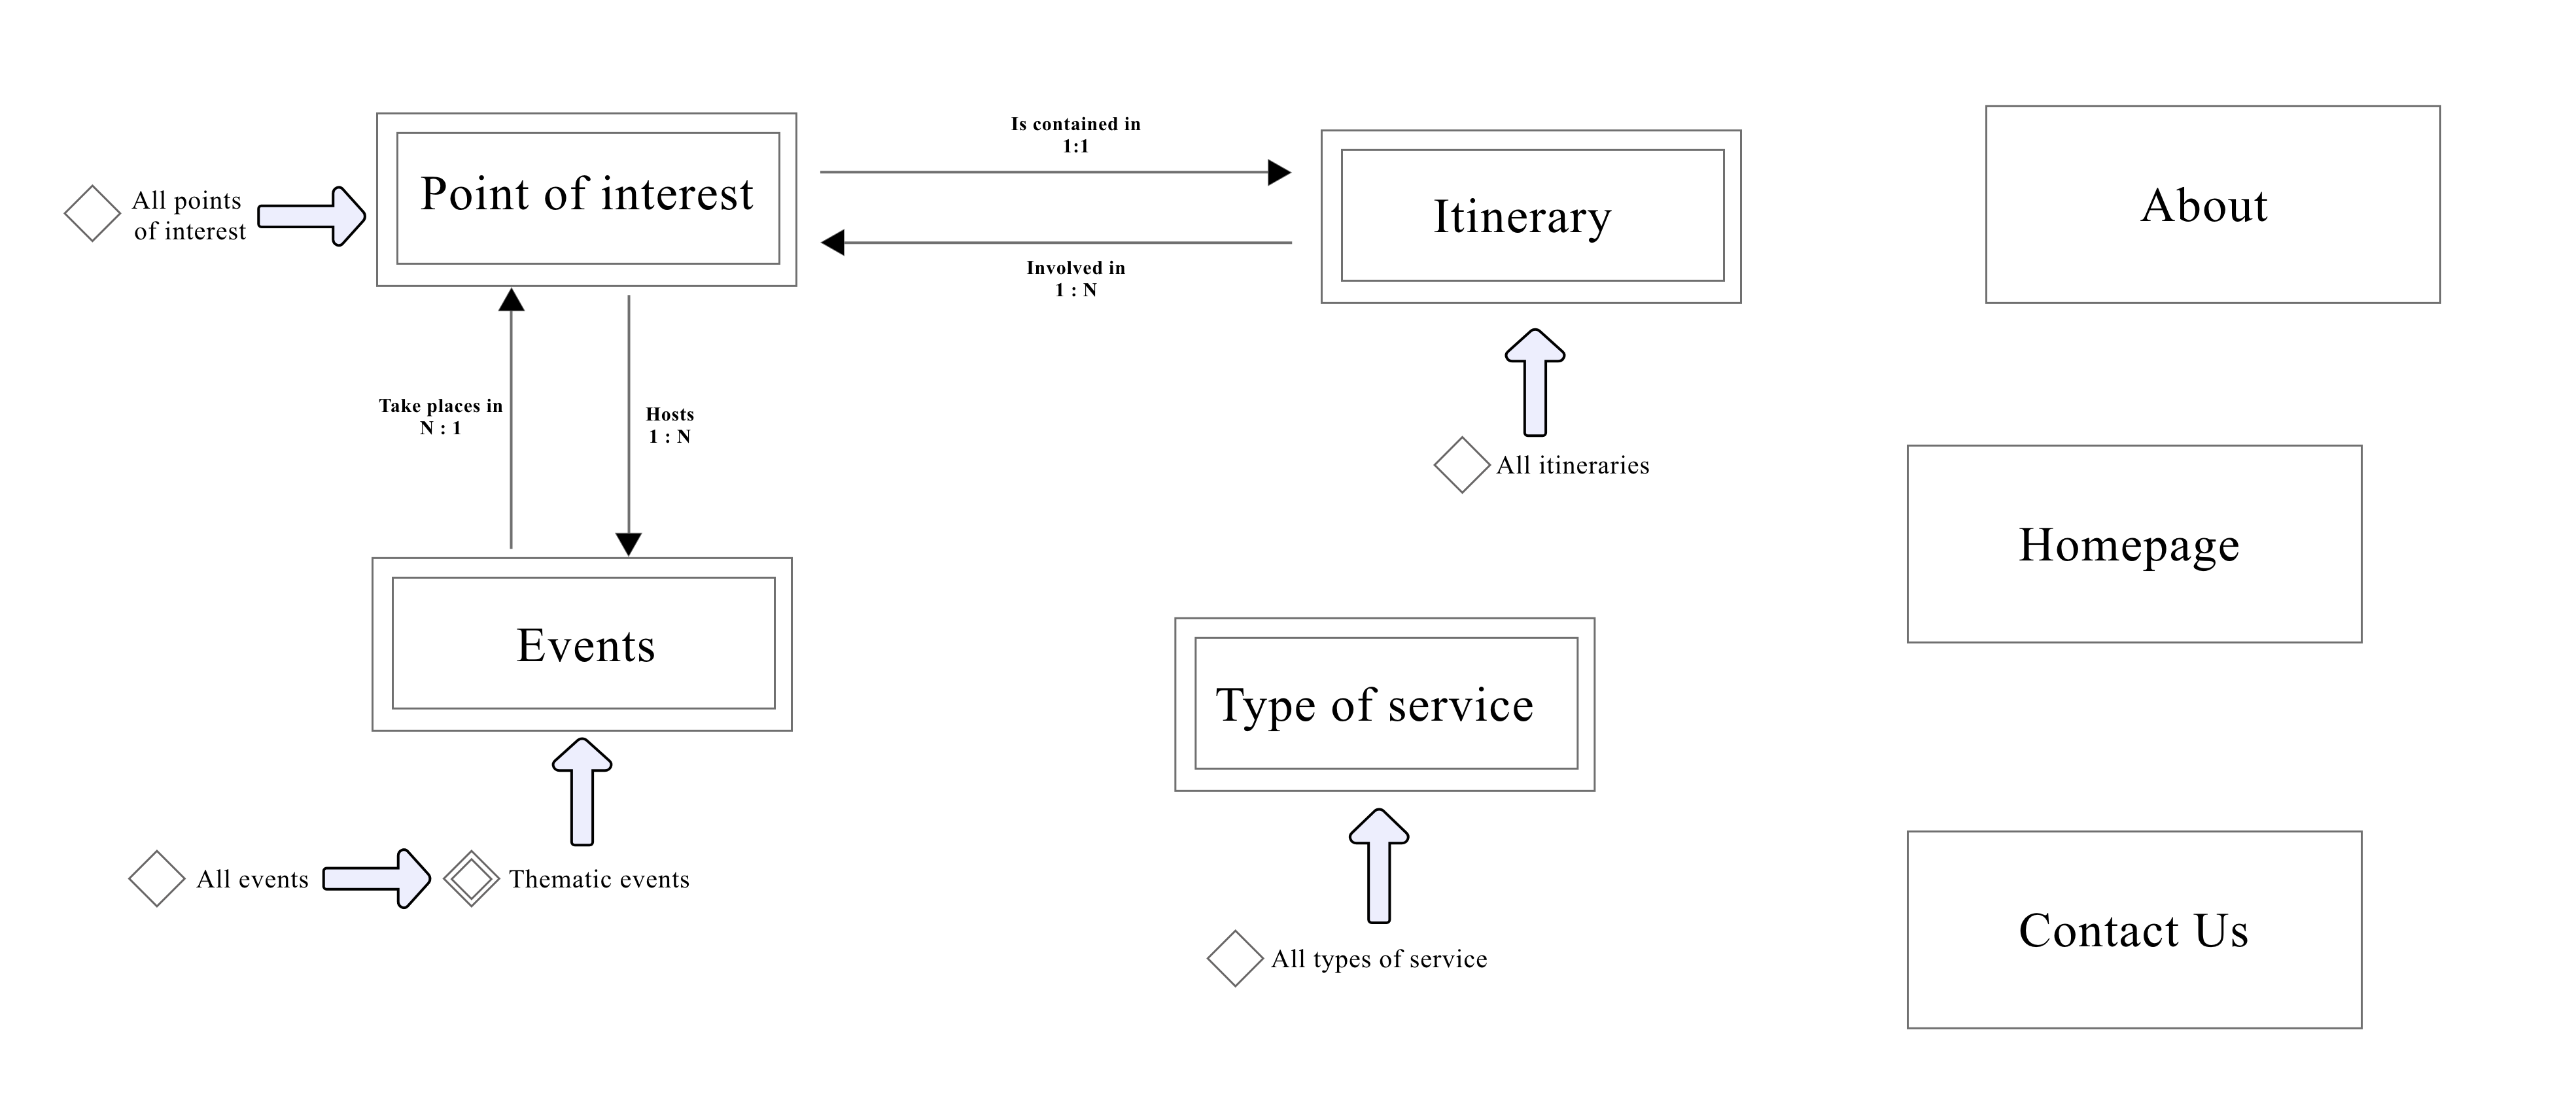
\includegraphics[width=\textwidth]{assets/Tables/C-IDM.png}
        \caption{C-IDM schema}
    \end{center}
\end{figure}

\section{Content-in-the small}
\subsection{Introduction}
This section is dedicated to the second step of the design process, which is related to the analysis of "what we want to put" in our pages : in fact in the following tables are well explained all the items and their properties (in terms of type of variable).
The tables are inserted in a manner that try to highlight the hierarchy beyond the site.
\subsection{Tables}
\begin{figure}[H]
    \begin{center}
        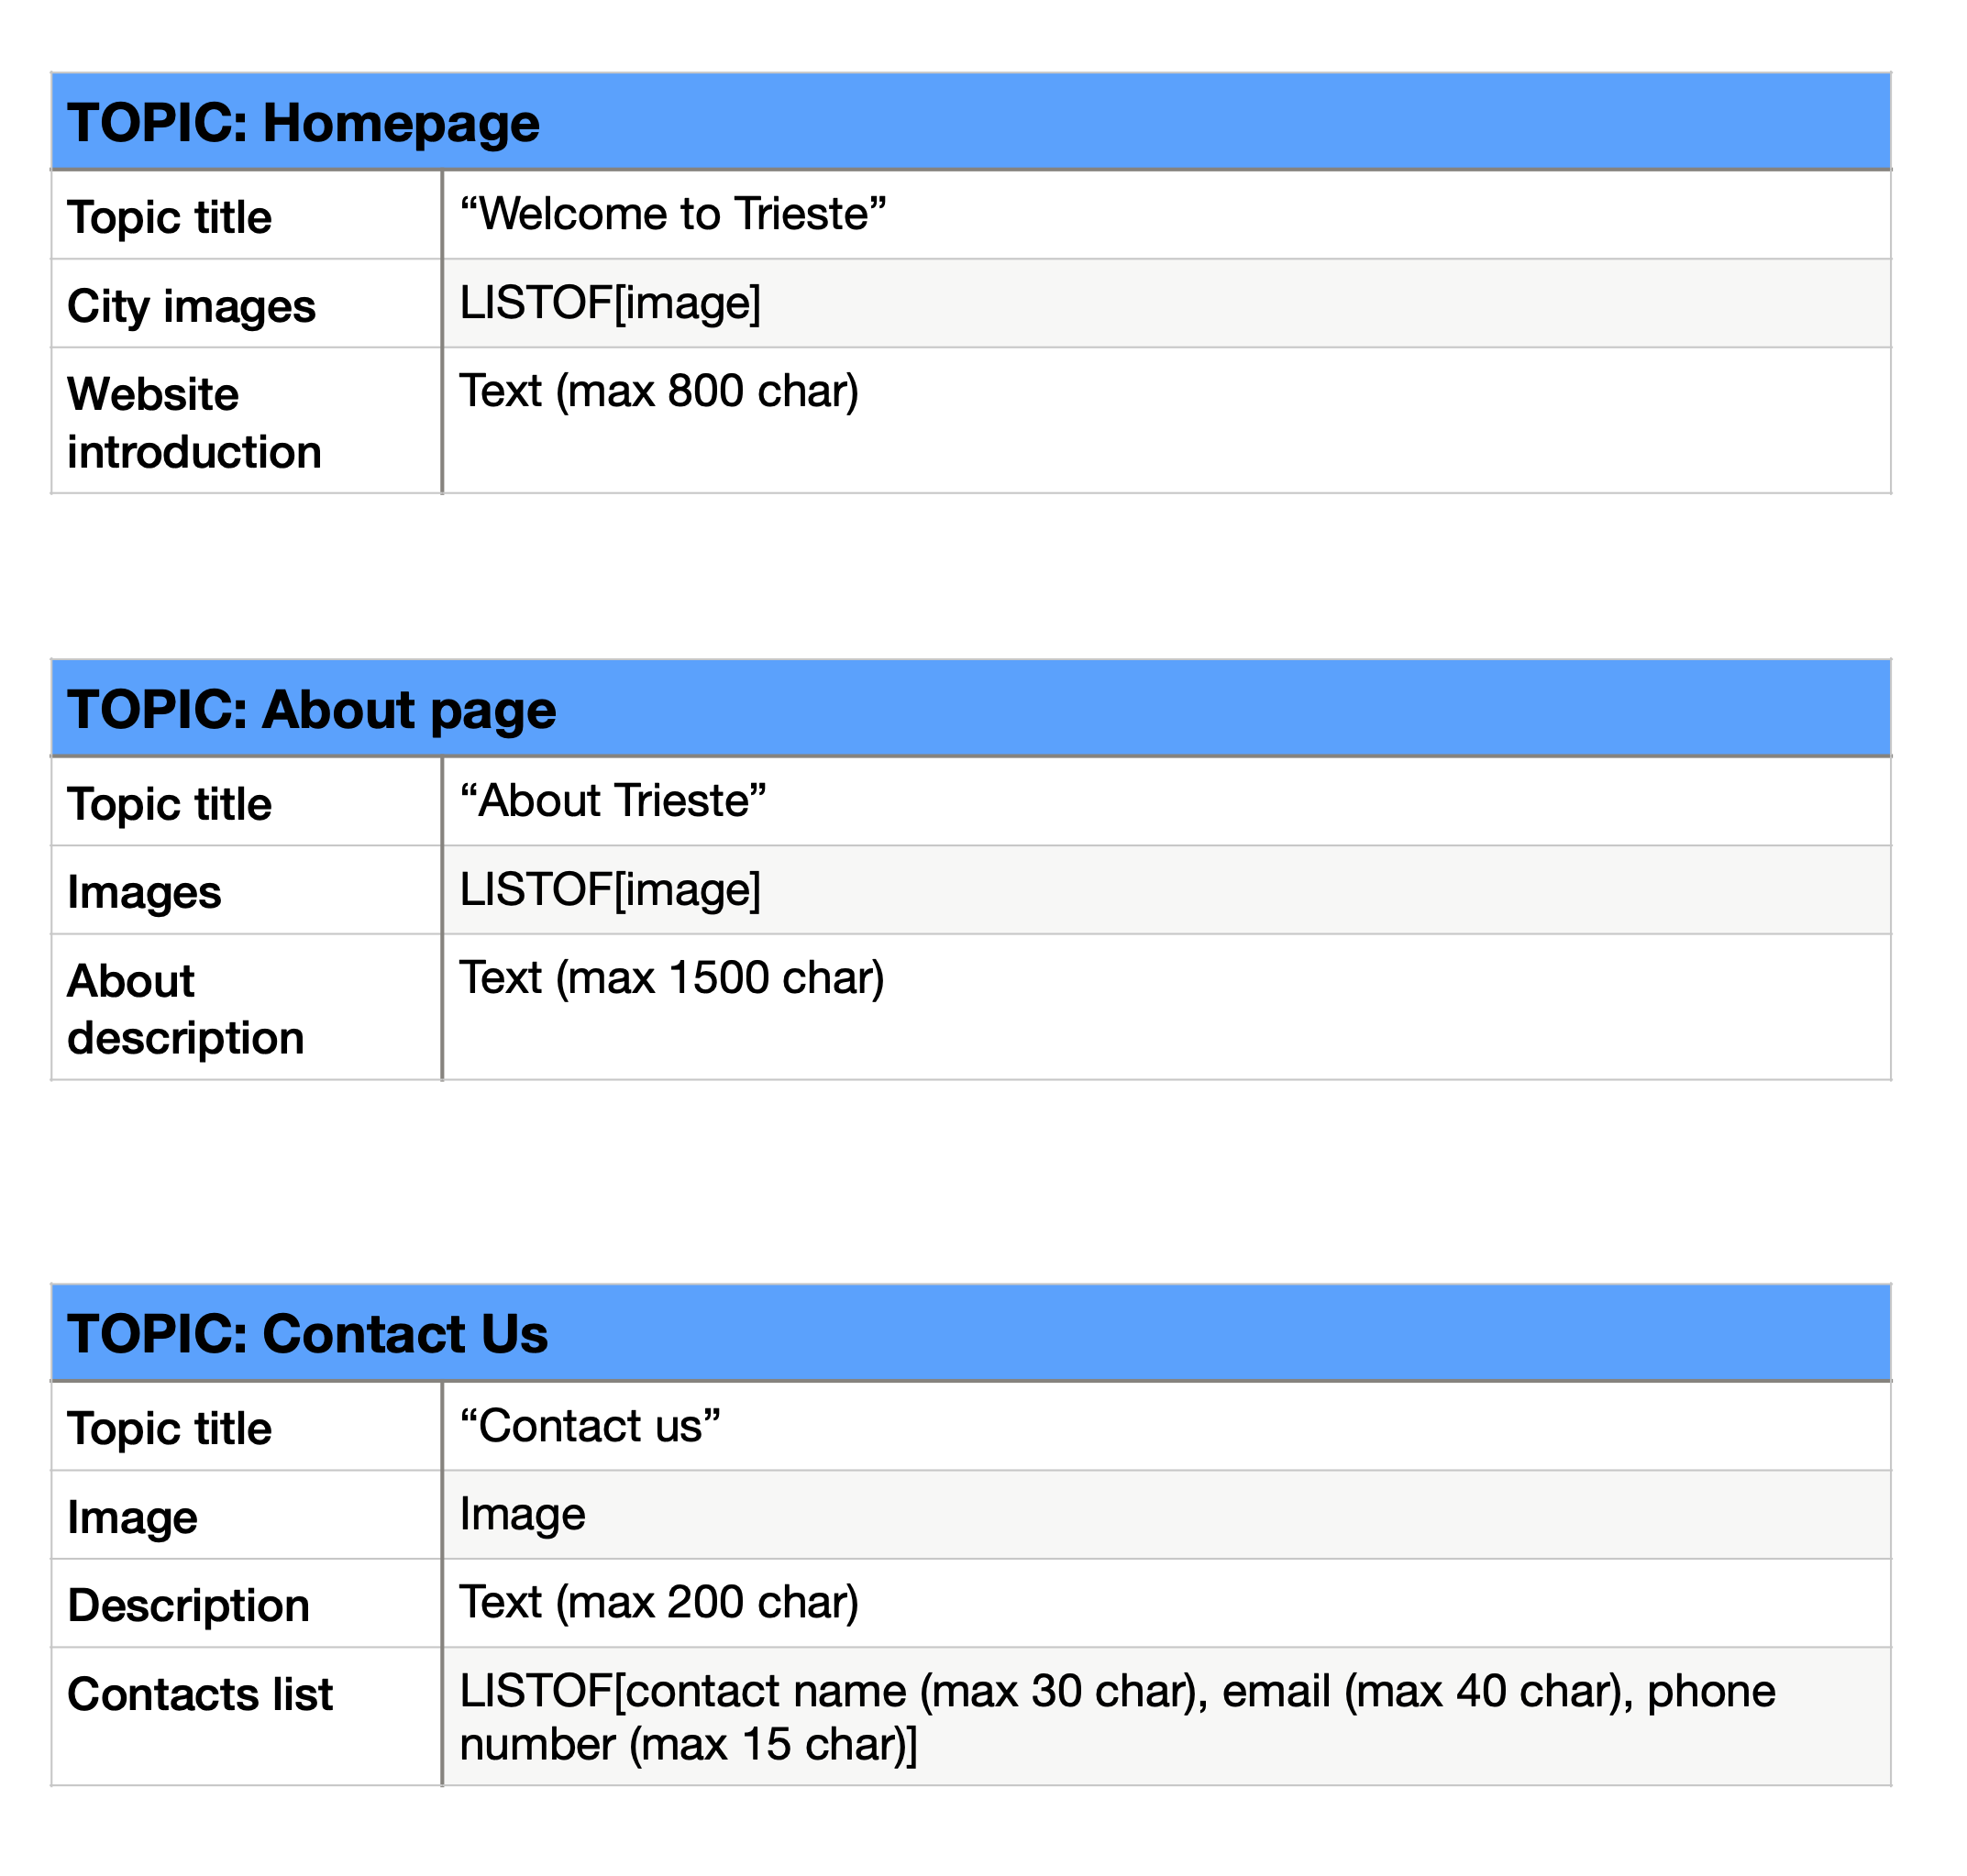
\includegraphics[width=\textwidth]{assets/Tables/Small/contentSmall1.png}
        \caption{Content in the small tables}
    \end{center}
\end{figure}

\begin{figure}[H]
    \begin{center}
        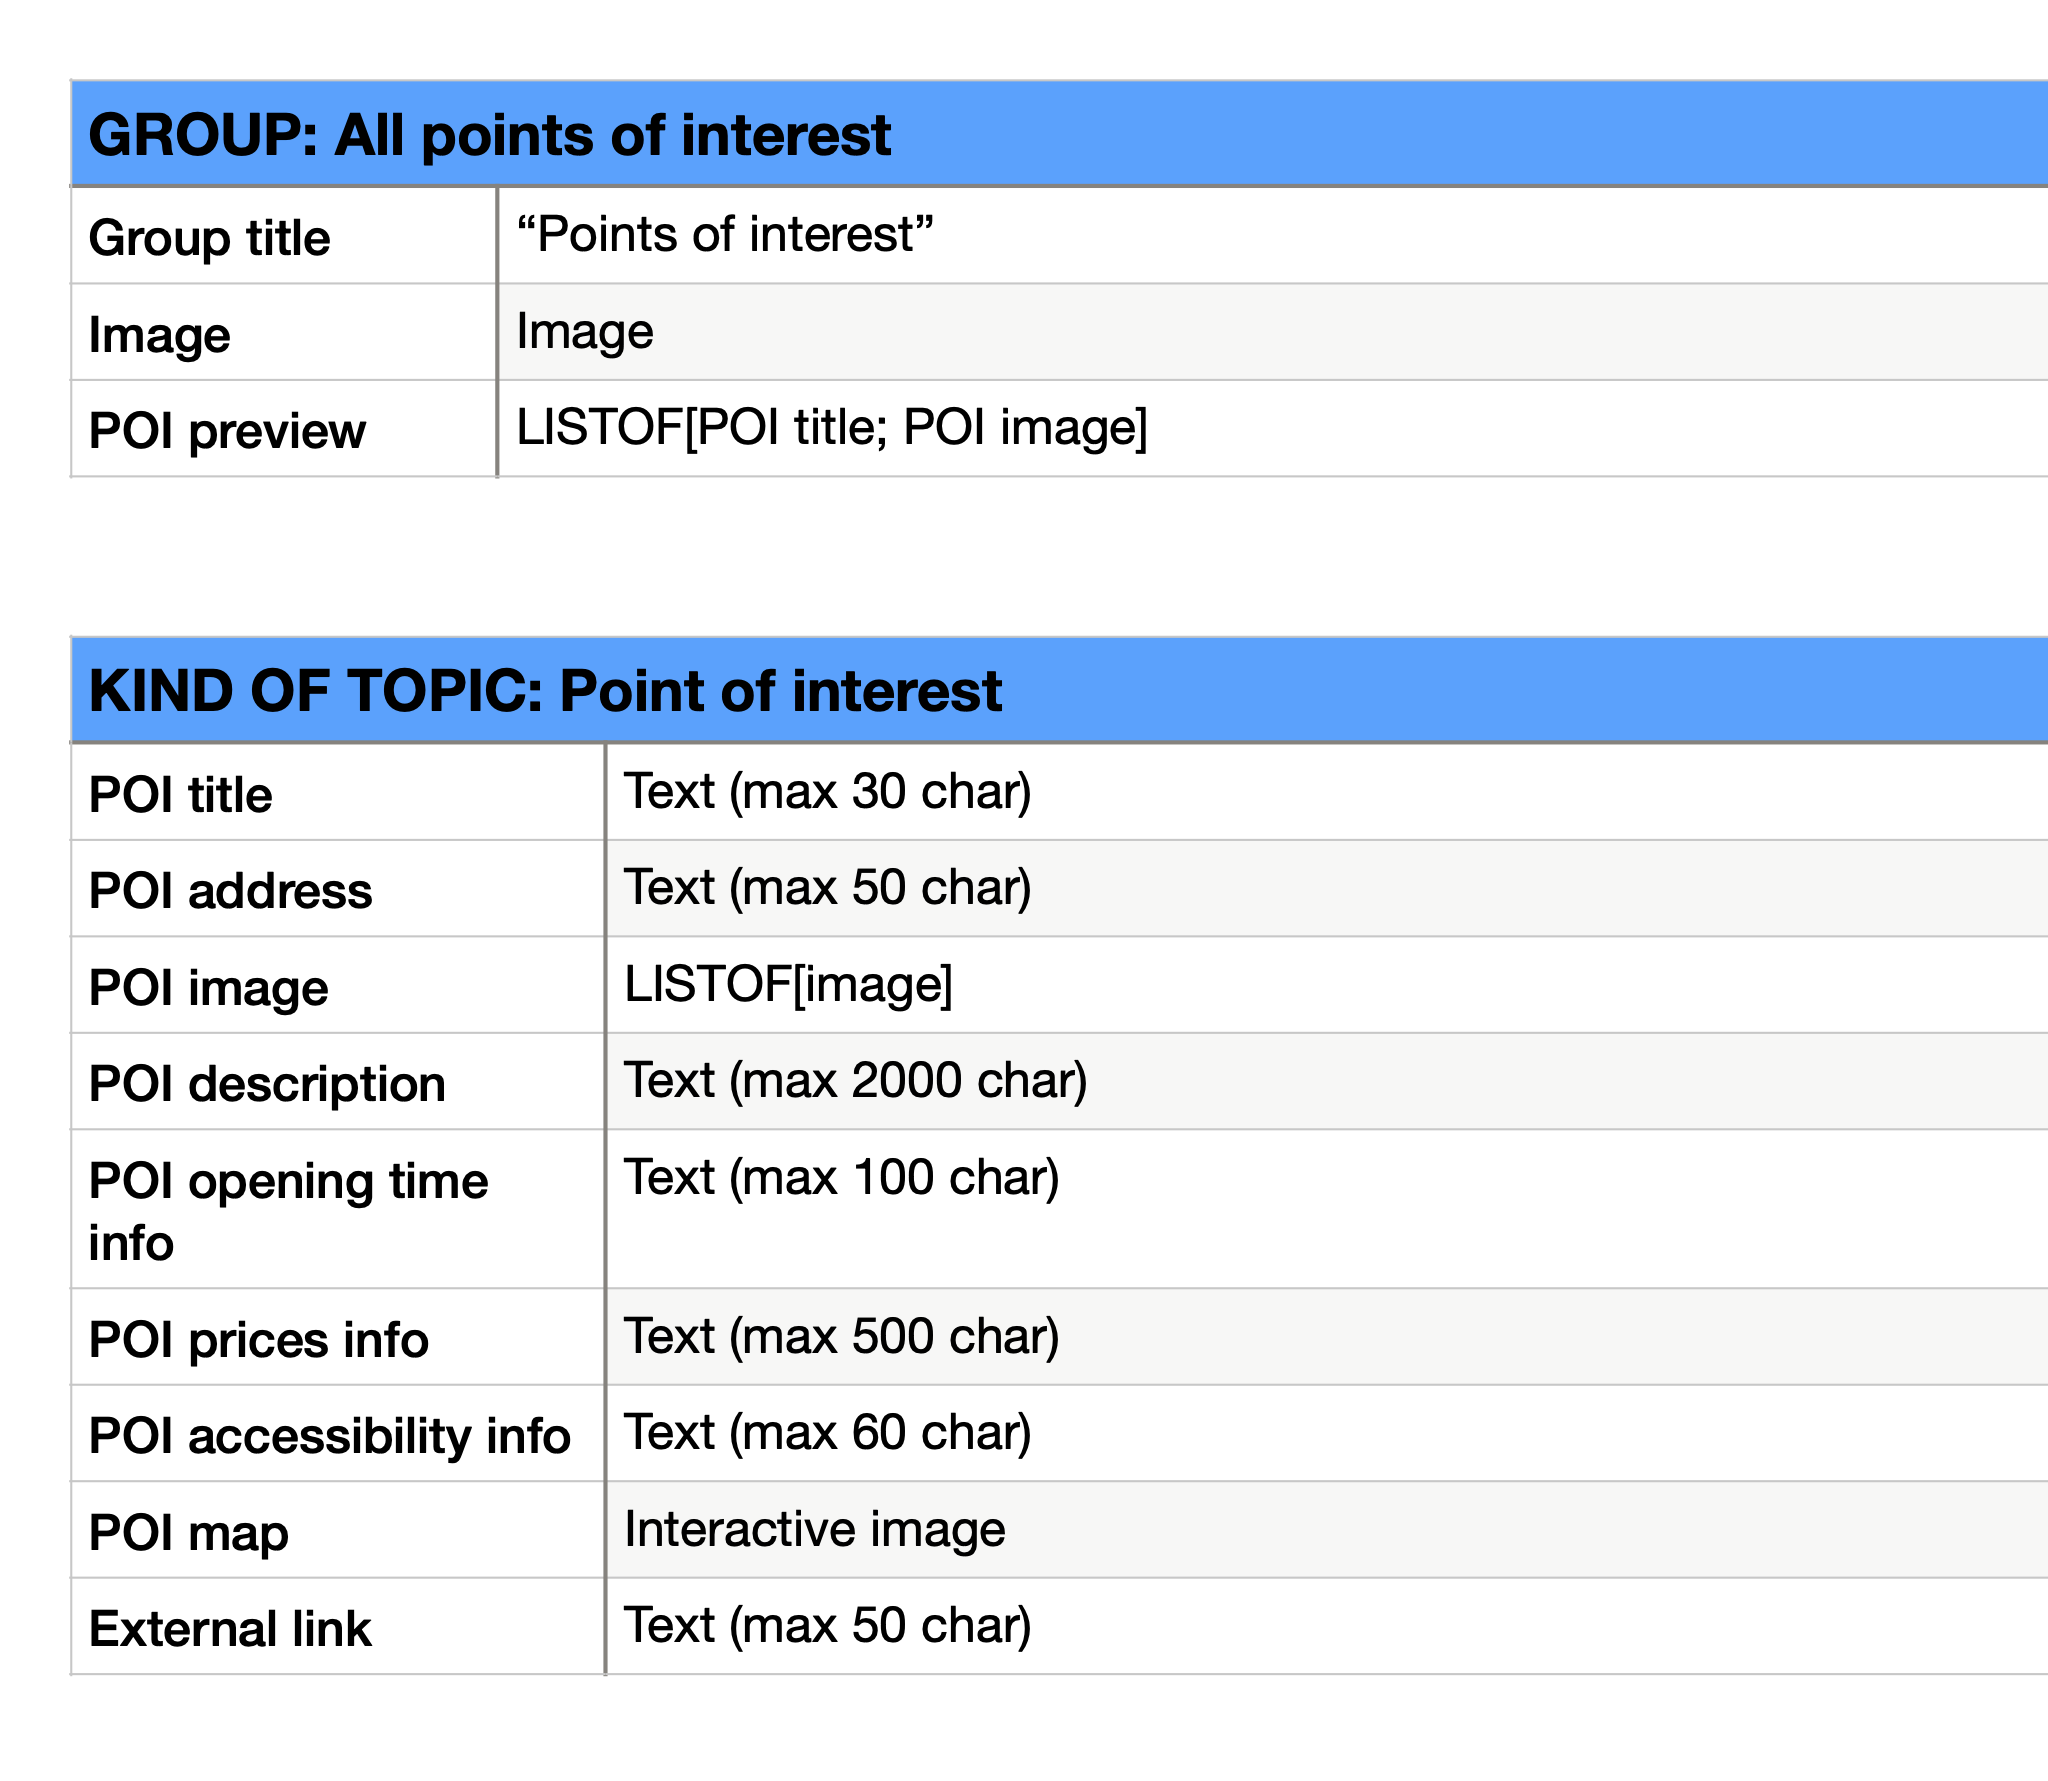
\includegraphics[width=\textwidth]{assets/Tables/Small/contentSmall2.png}
        \caption{Content in the small tables}
    \end{center}
\end{figure}

\begin{figure}[H]
    \begin{center}
        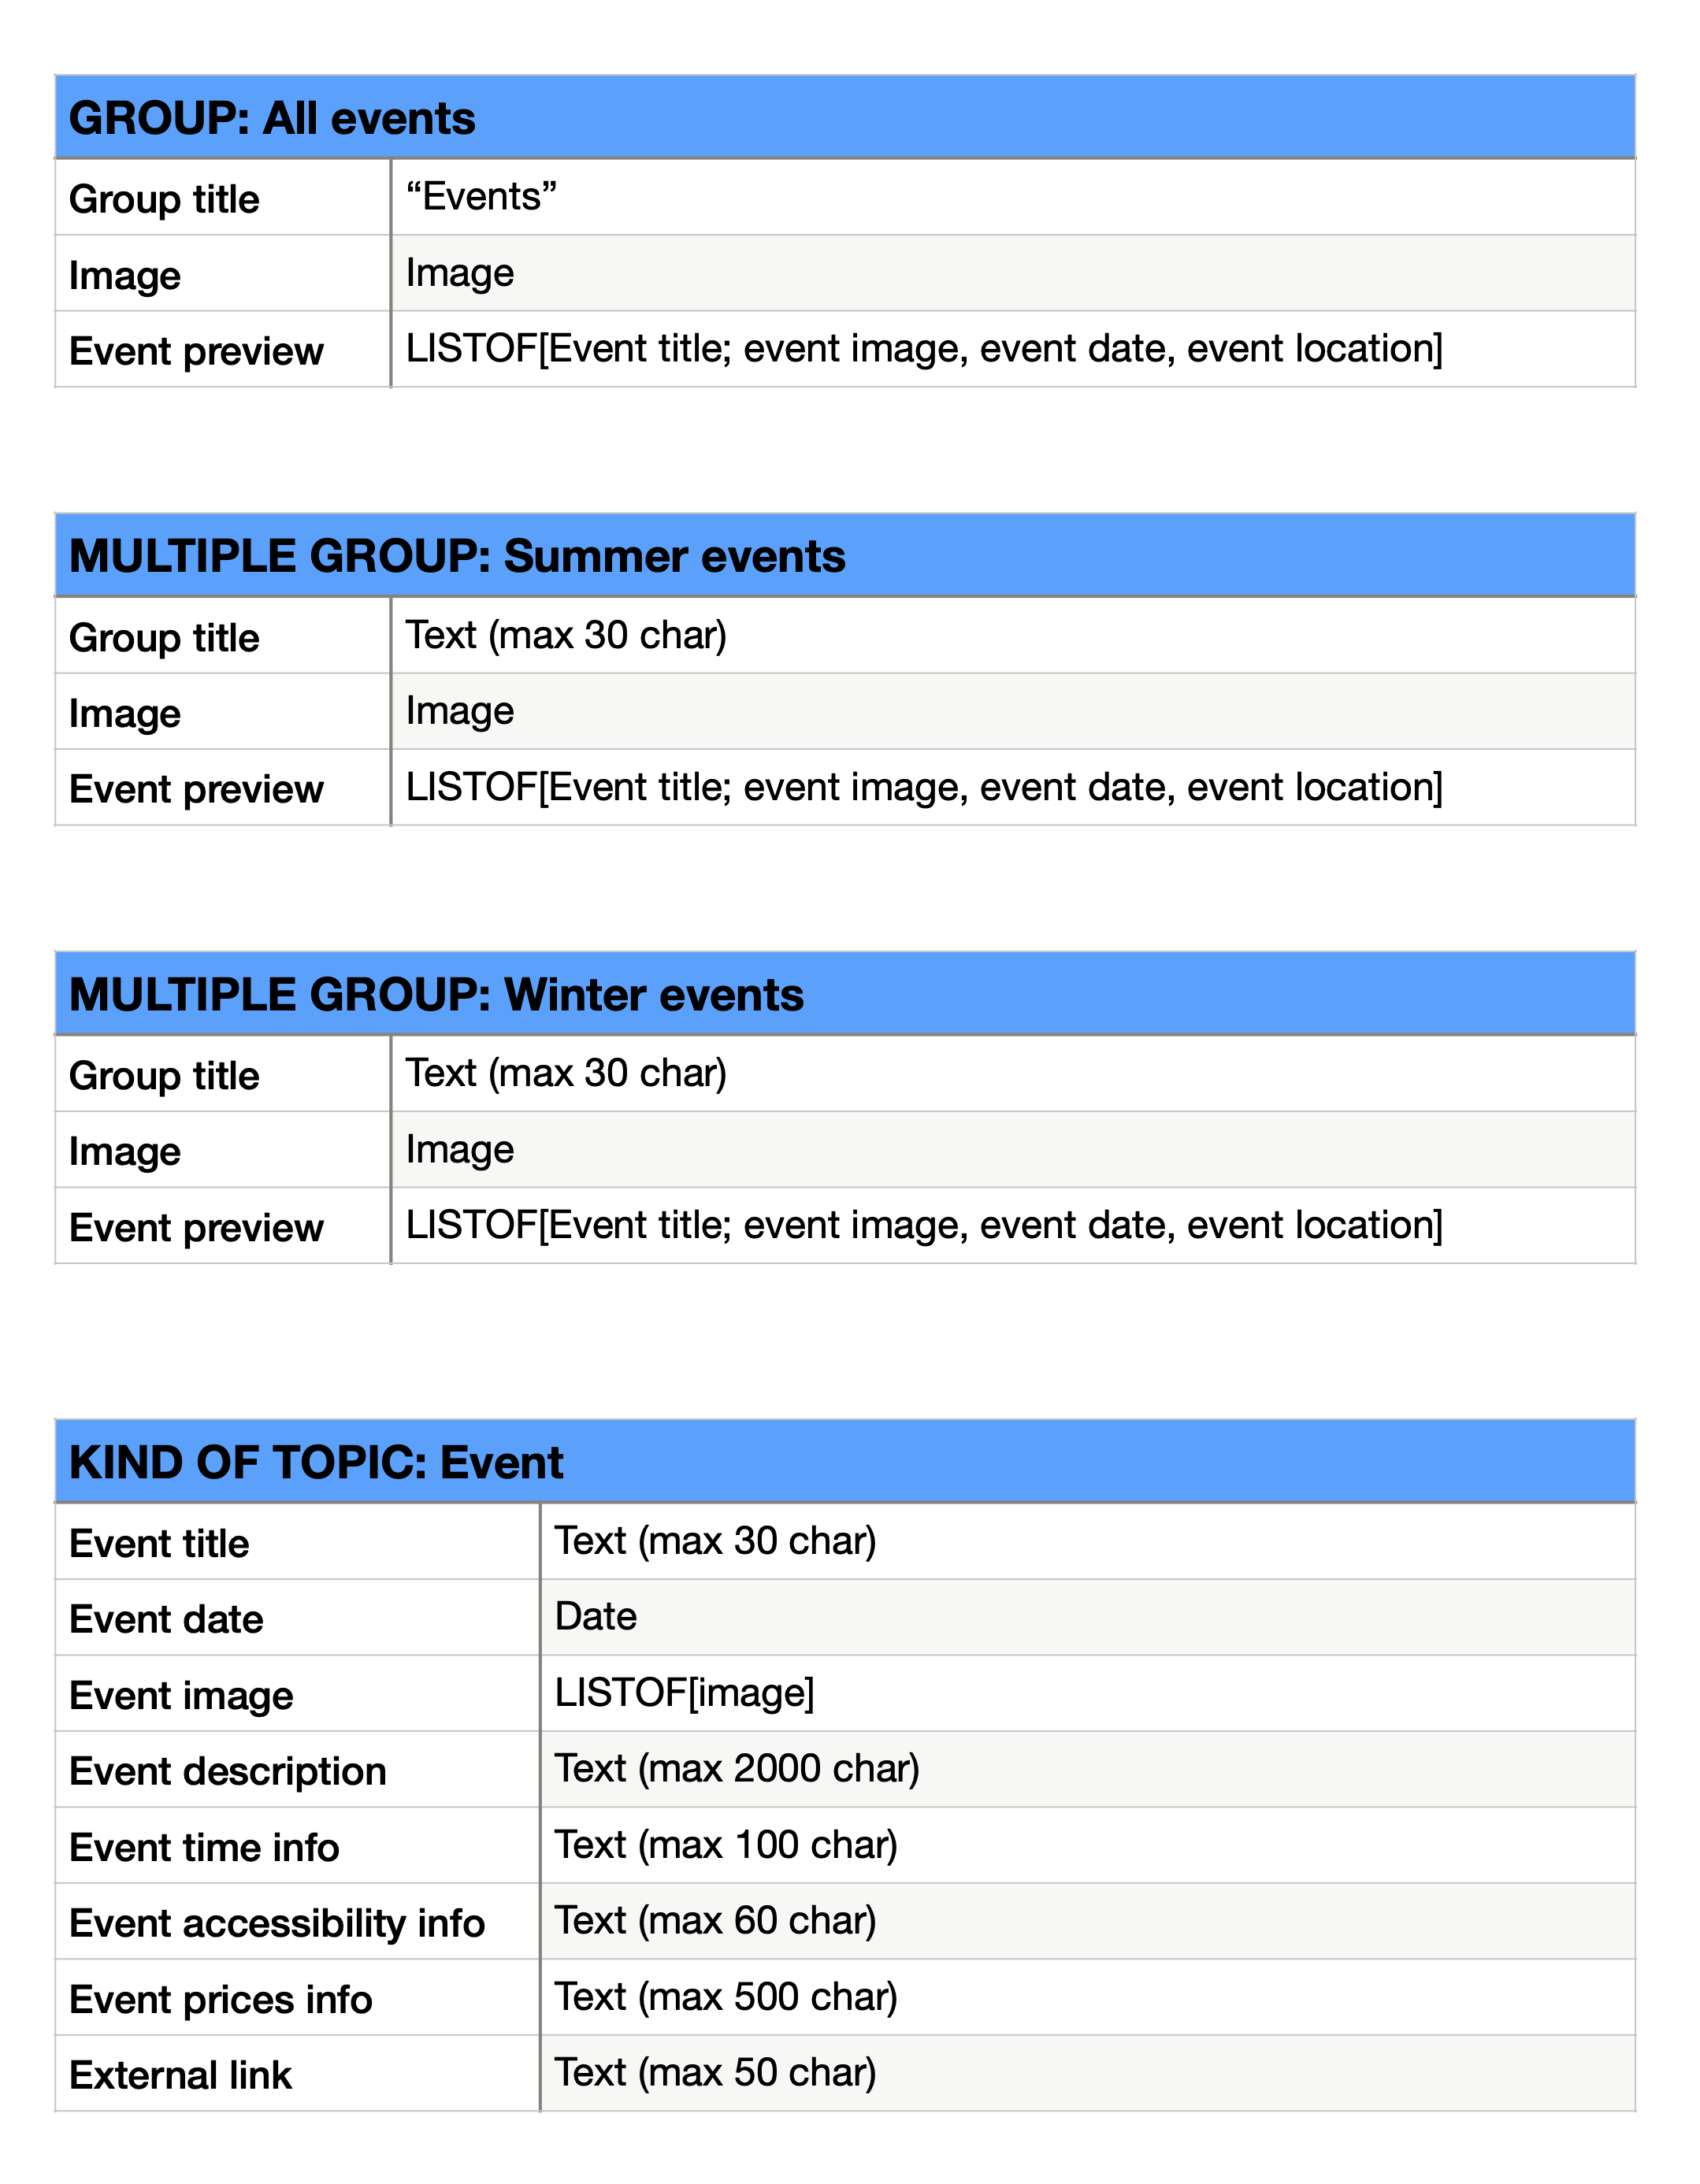
\includegraphics[width=\textwidth]{assets/Tables/Small/contentSmall3.png}
        \caption{Content in the small tables}
    \end{center}
\end{figure}

\begin{figure}[H]
    \begin{center}
        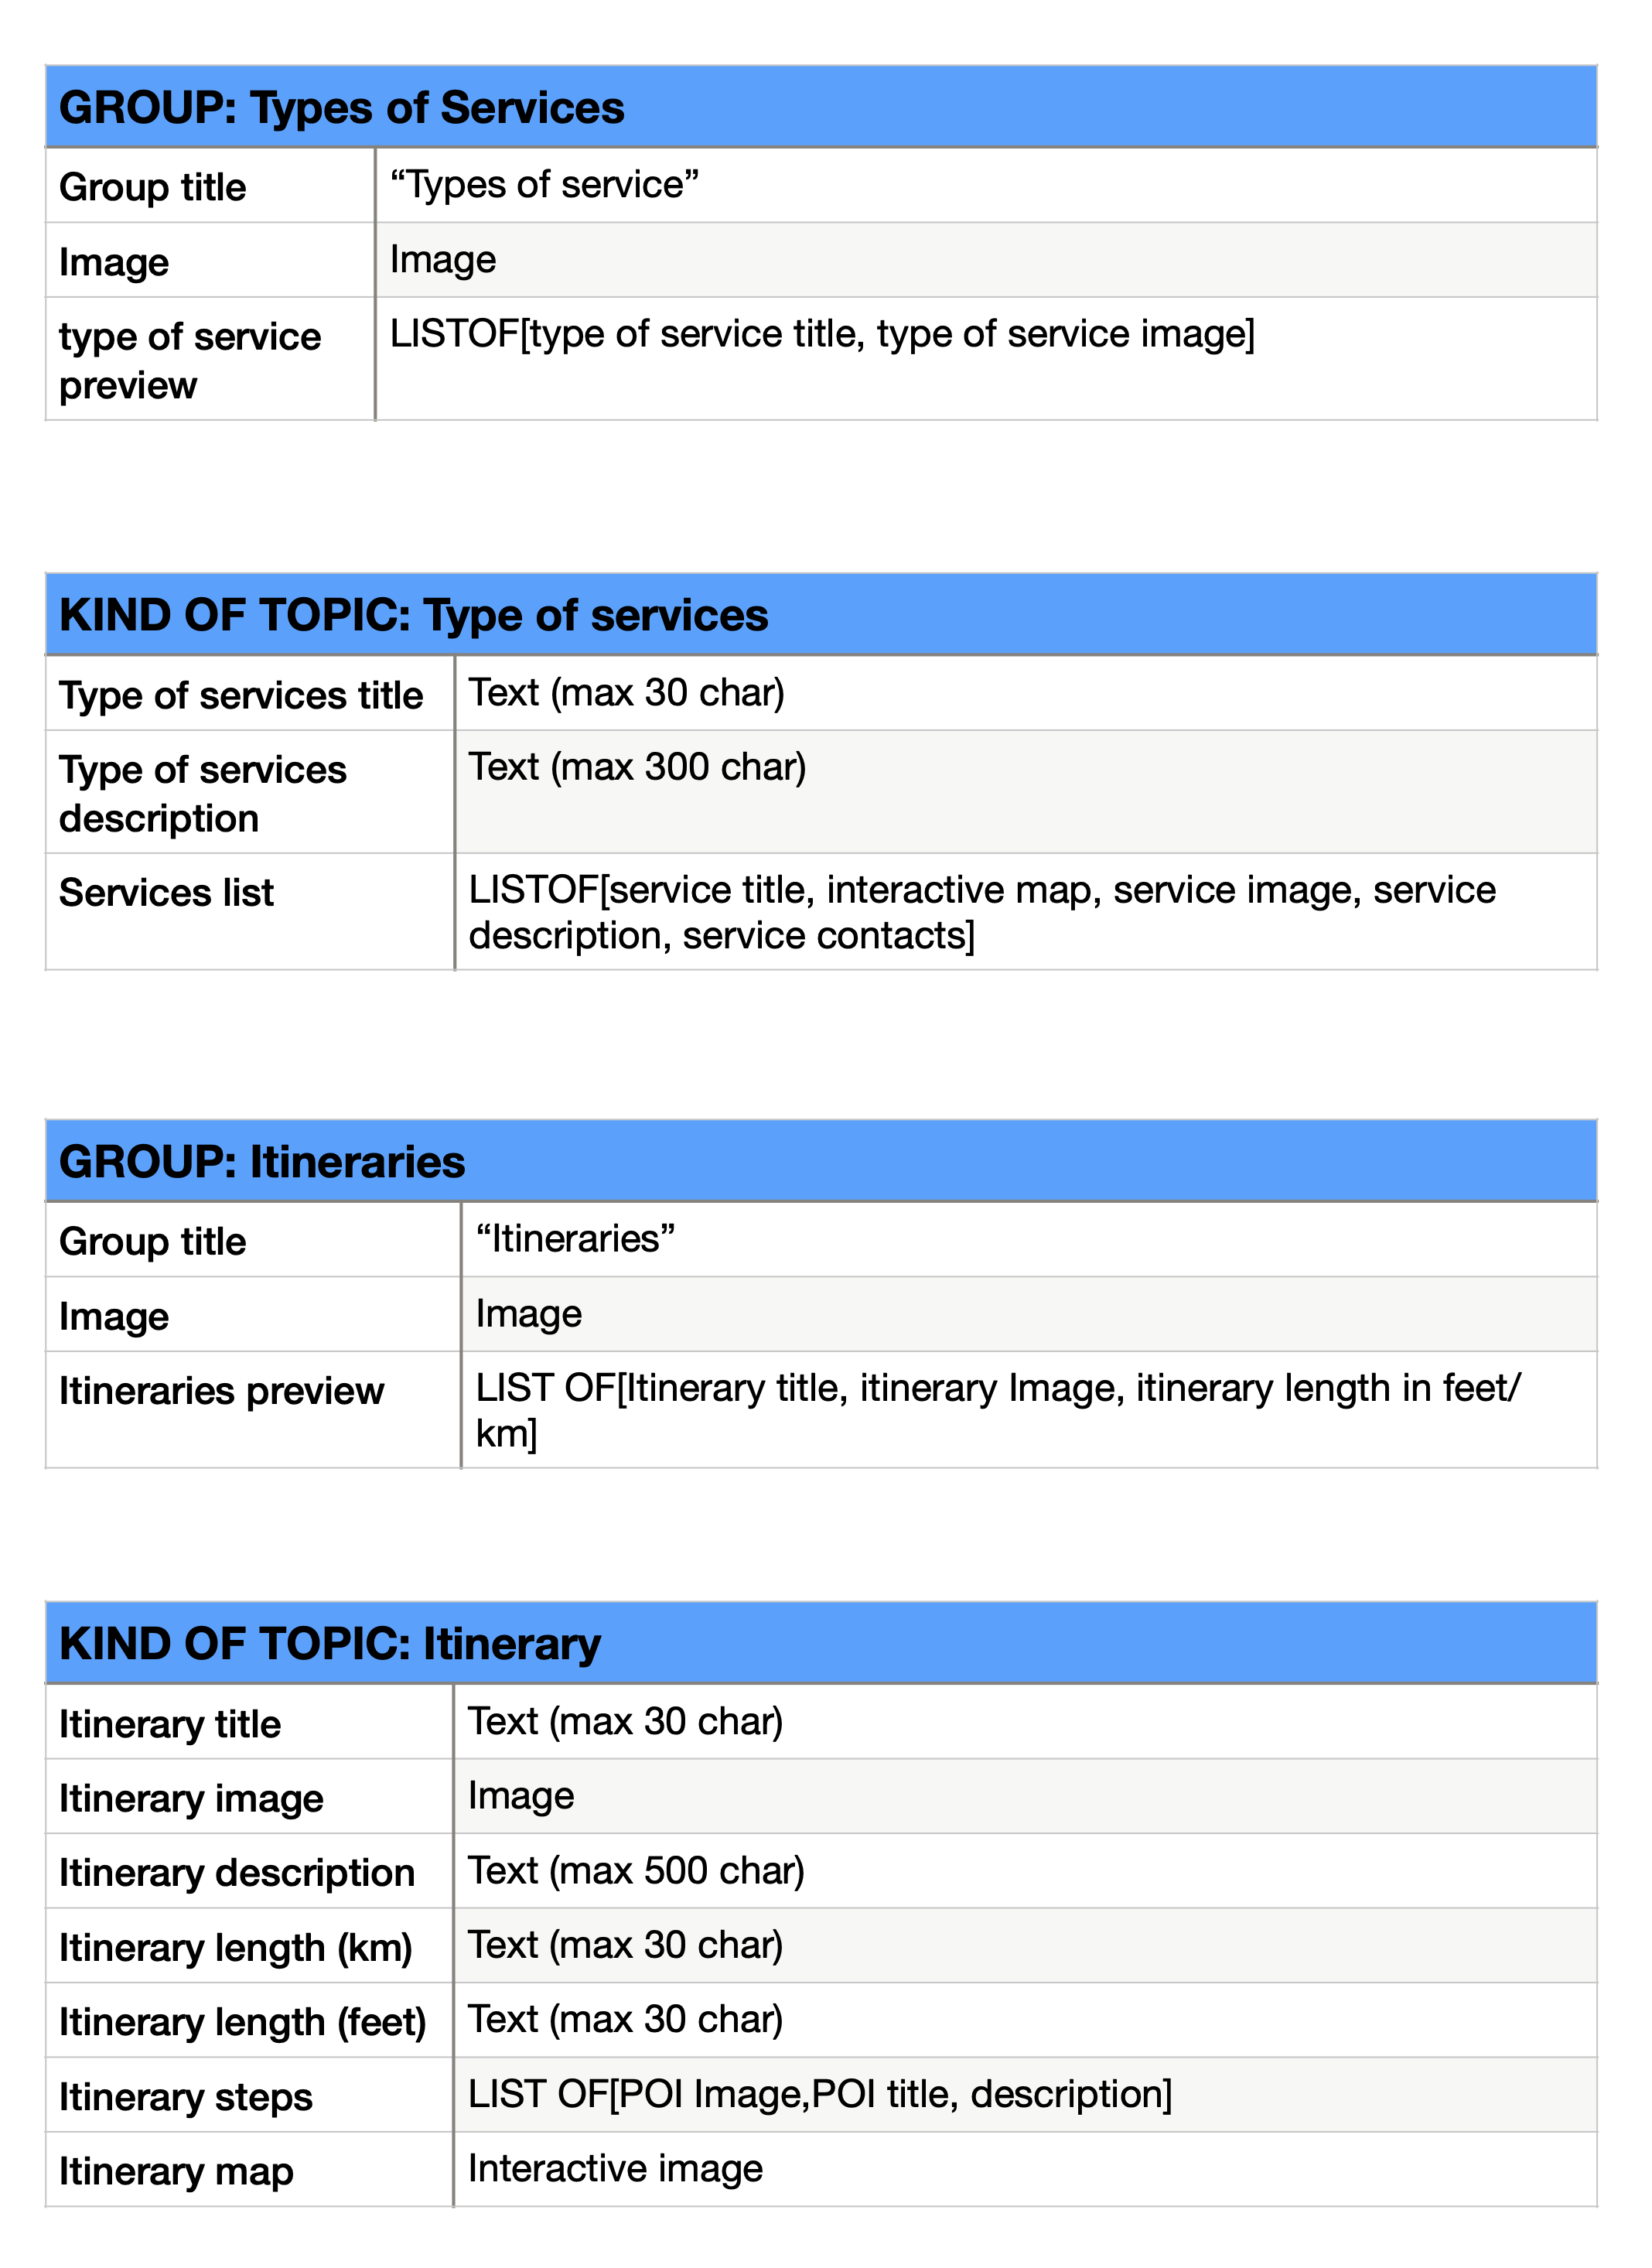
\includegraphics[width=\textwidth]{assets/Tables/Small/contentSmall4.png}
        \caption{Content in the small tables}
    \end{center}
\end{figure}

\newpage
\section{Database design}
We decide to insert in the database only the data related to multiple topic pages and group of topics pages because they are the most articulated ones (their content is dynamically changing according to the context) with respect to the homepage, about and contacts, which are basically static pages.
\subsection{ER-Diagram}
The Entity-Relationship Diagram is a theoretical model used to show at an high-level-abstraction the relationships among the database entities and to list their attributes.
\begin{figure}[H]
    \begin{center}
        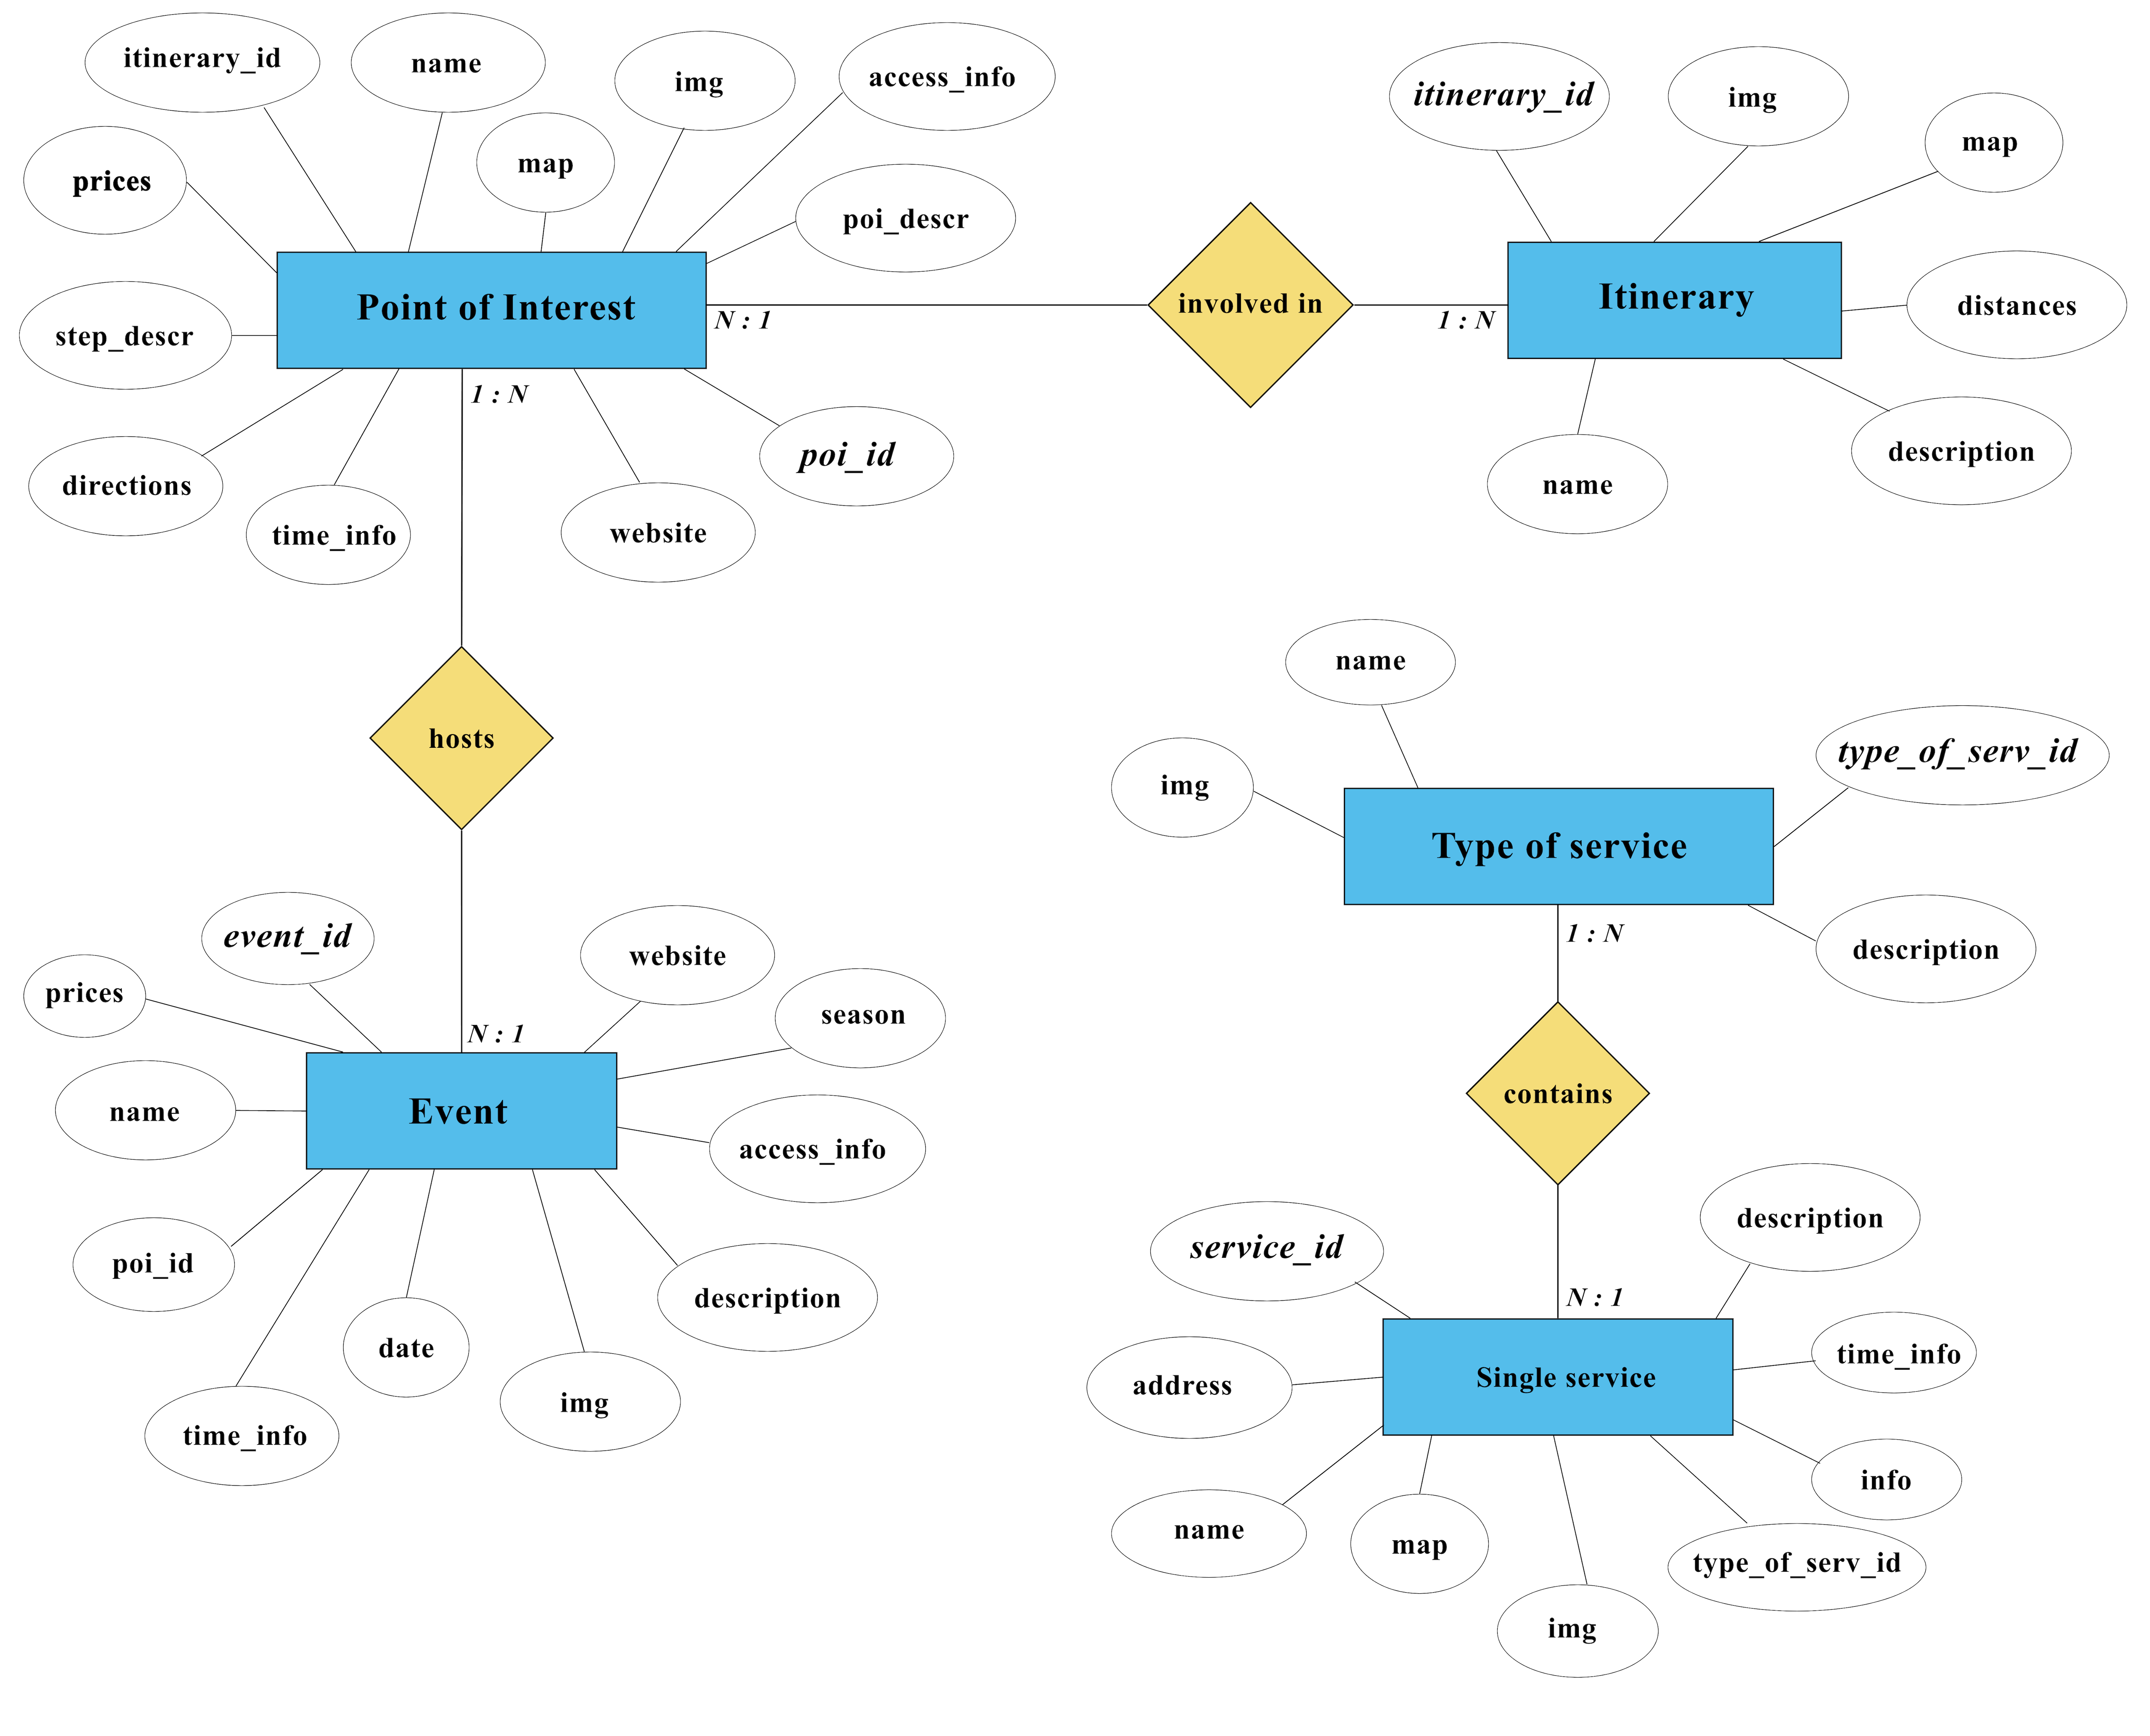
\includegraphics[width=\textwidth]{assets/Tables/ER-Diagram.png}
        \caption{Entity-Relationship diagram}
    \end{center}
\end{figure}
\subsection{Data tables}
Data tables derive from the previous diagram: in fact they deeply describe all the attributes in term of variable's type and the keys (primary and foreign) of each entity.
\begin{figure}[H]
    \begin{center}
        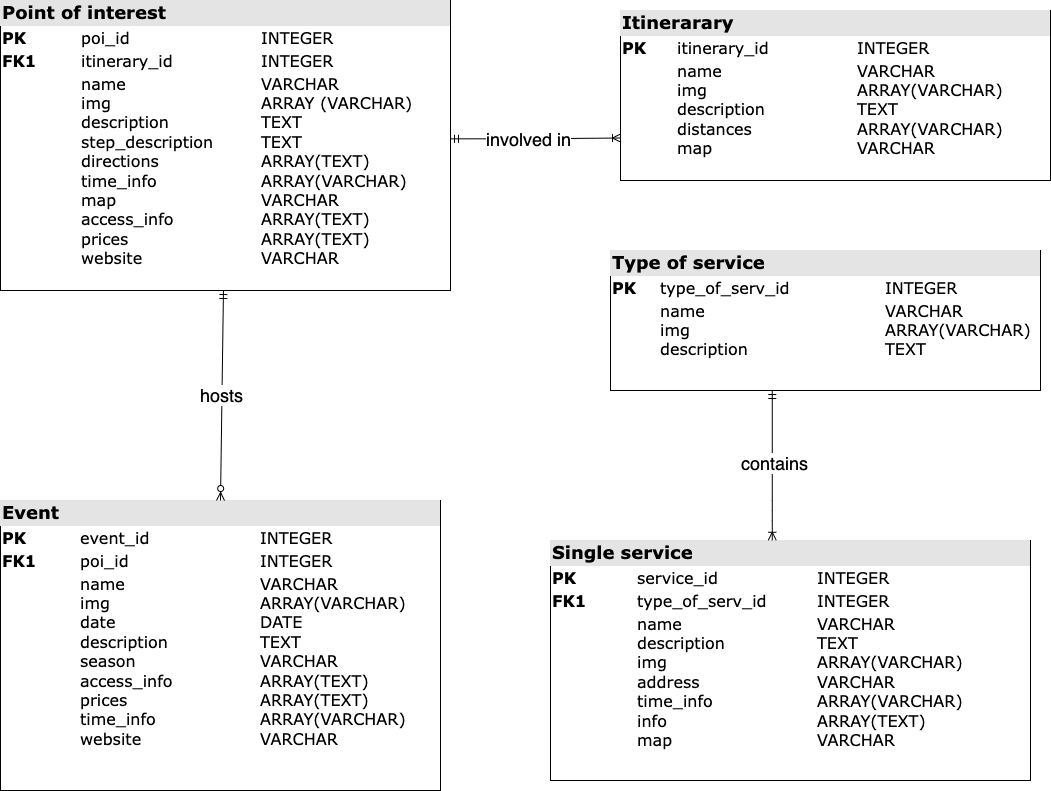
\includegraphics[width=\textwidth]{assets/Tables/dataTables.png}
        \caption{Data tables of the DB}
    \end{center}
\end{figure}

\newpage
\section{Abstract pages}
\subsection{Introduction}
Abstract pages are the last tables between the design work and the implementation one: in fact the following tables contains the accurate description of all the items we projected for all the pages, in order to give a detailed explanation of "what we expect to see" in our website. In real life, abstract pages are delivered to a design group who merge the conceptual organization and the aesthetic factor to achieve a good compromise in terms of Usability, Readability and Aesthetic. \\
The abstract pages contain also the classified type of links for each page (and the related navigation pattern, if used) in order to give a general view of all the connections that are needed for each page.
\subsection{Tables}
\begin{figure}[H]
    \begin{center}
        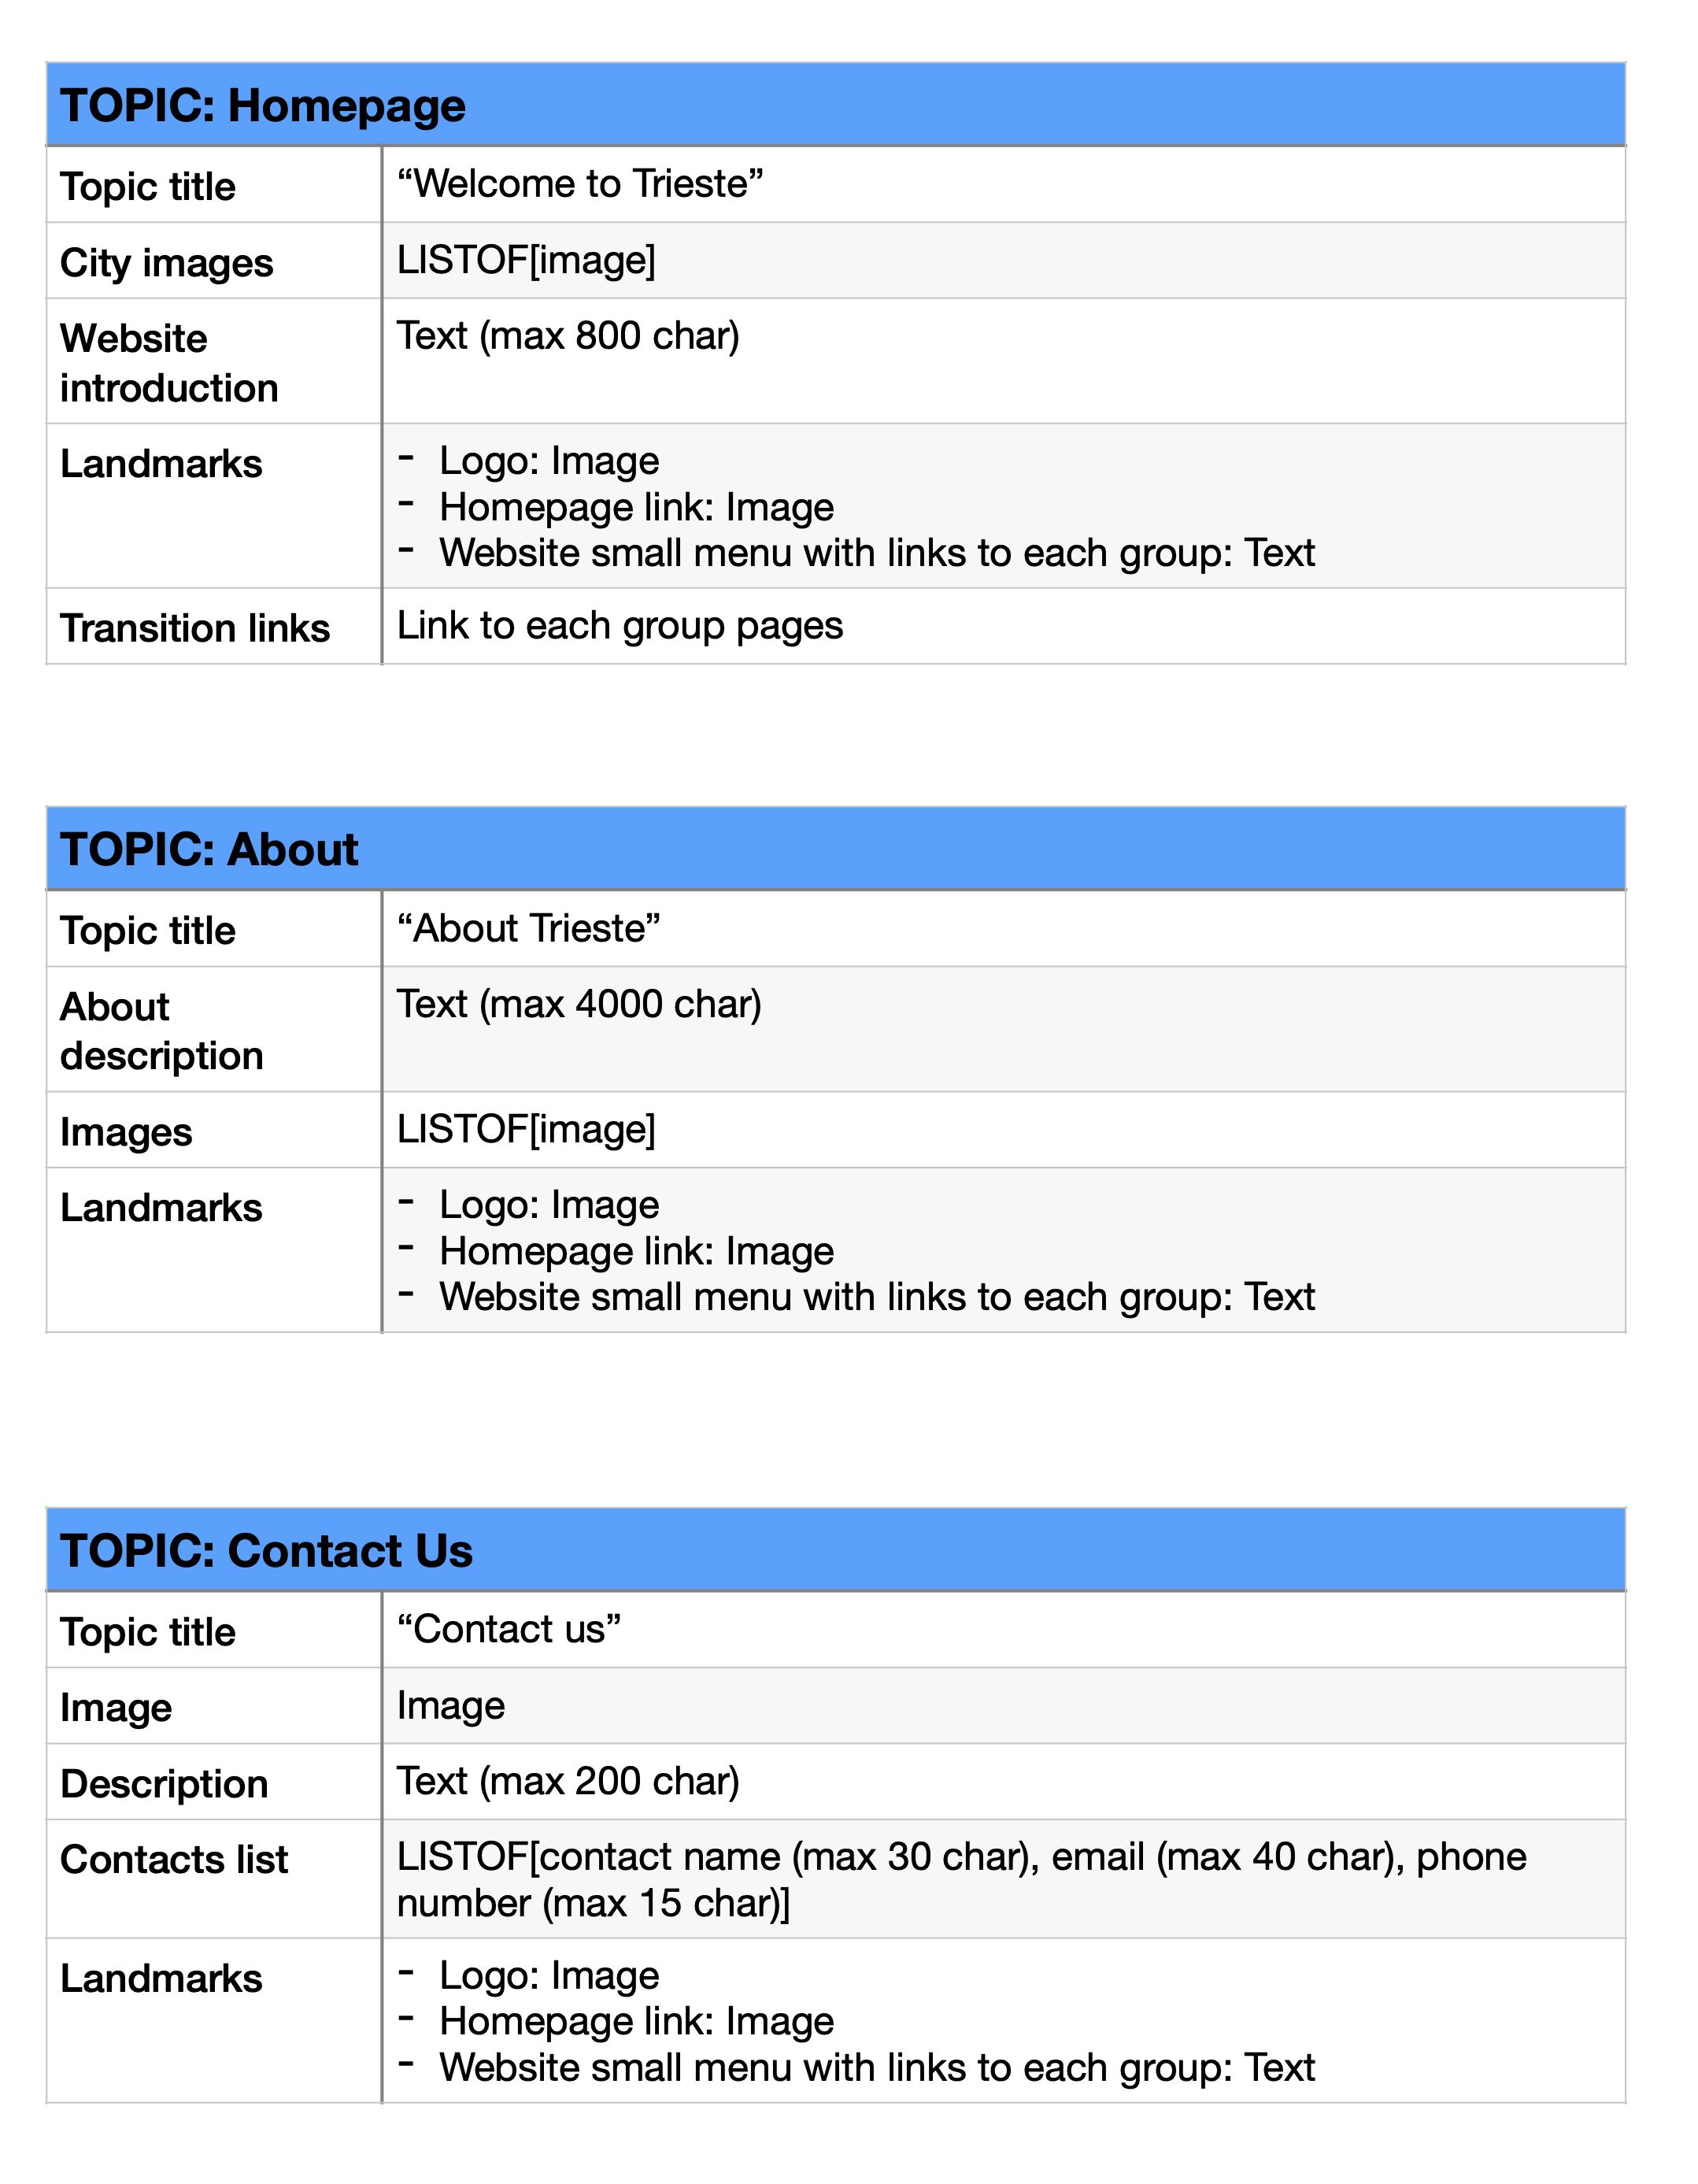
\includegraphics[width=\textwidth]{assets/Tables/Abstract/abstractPage1.png}
        \caption{Abstract pages}
    \end{center}
\end{figure}

\begin{figure}[H]
    \begin{center}
        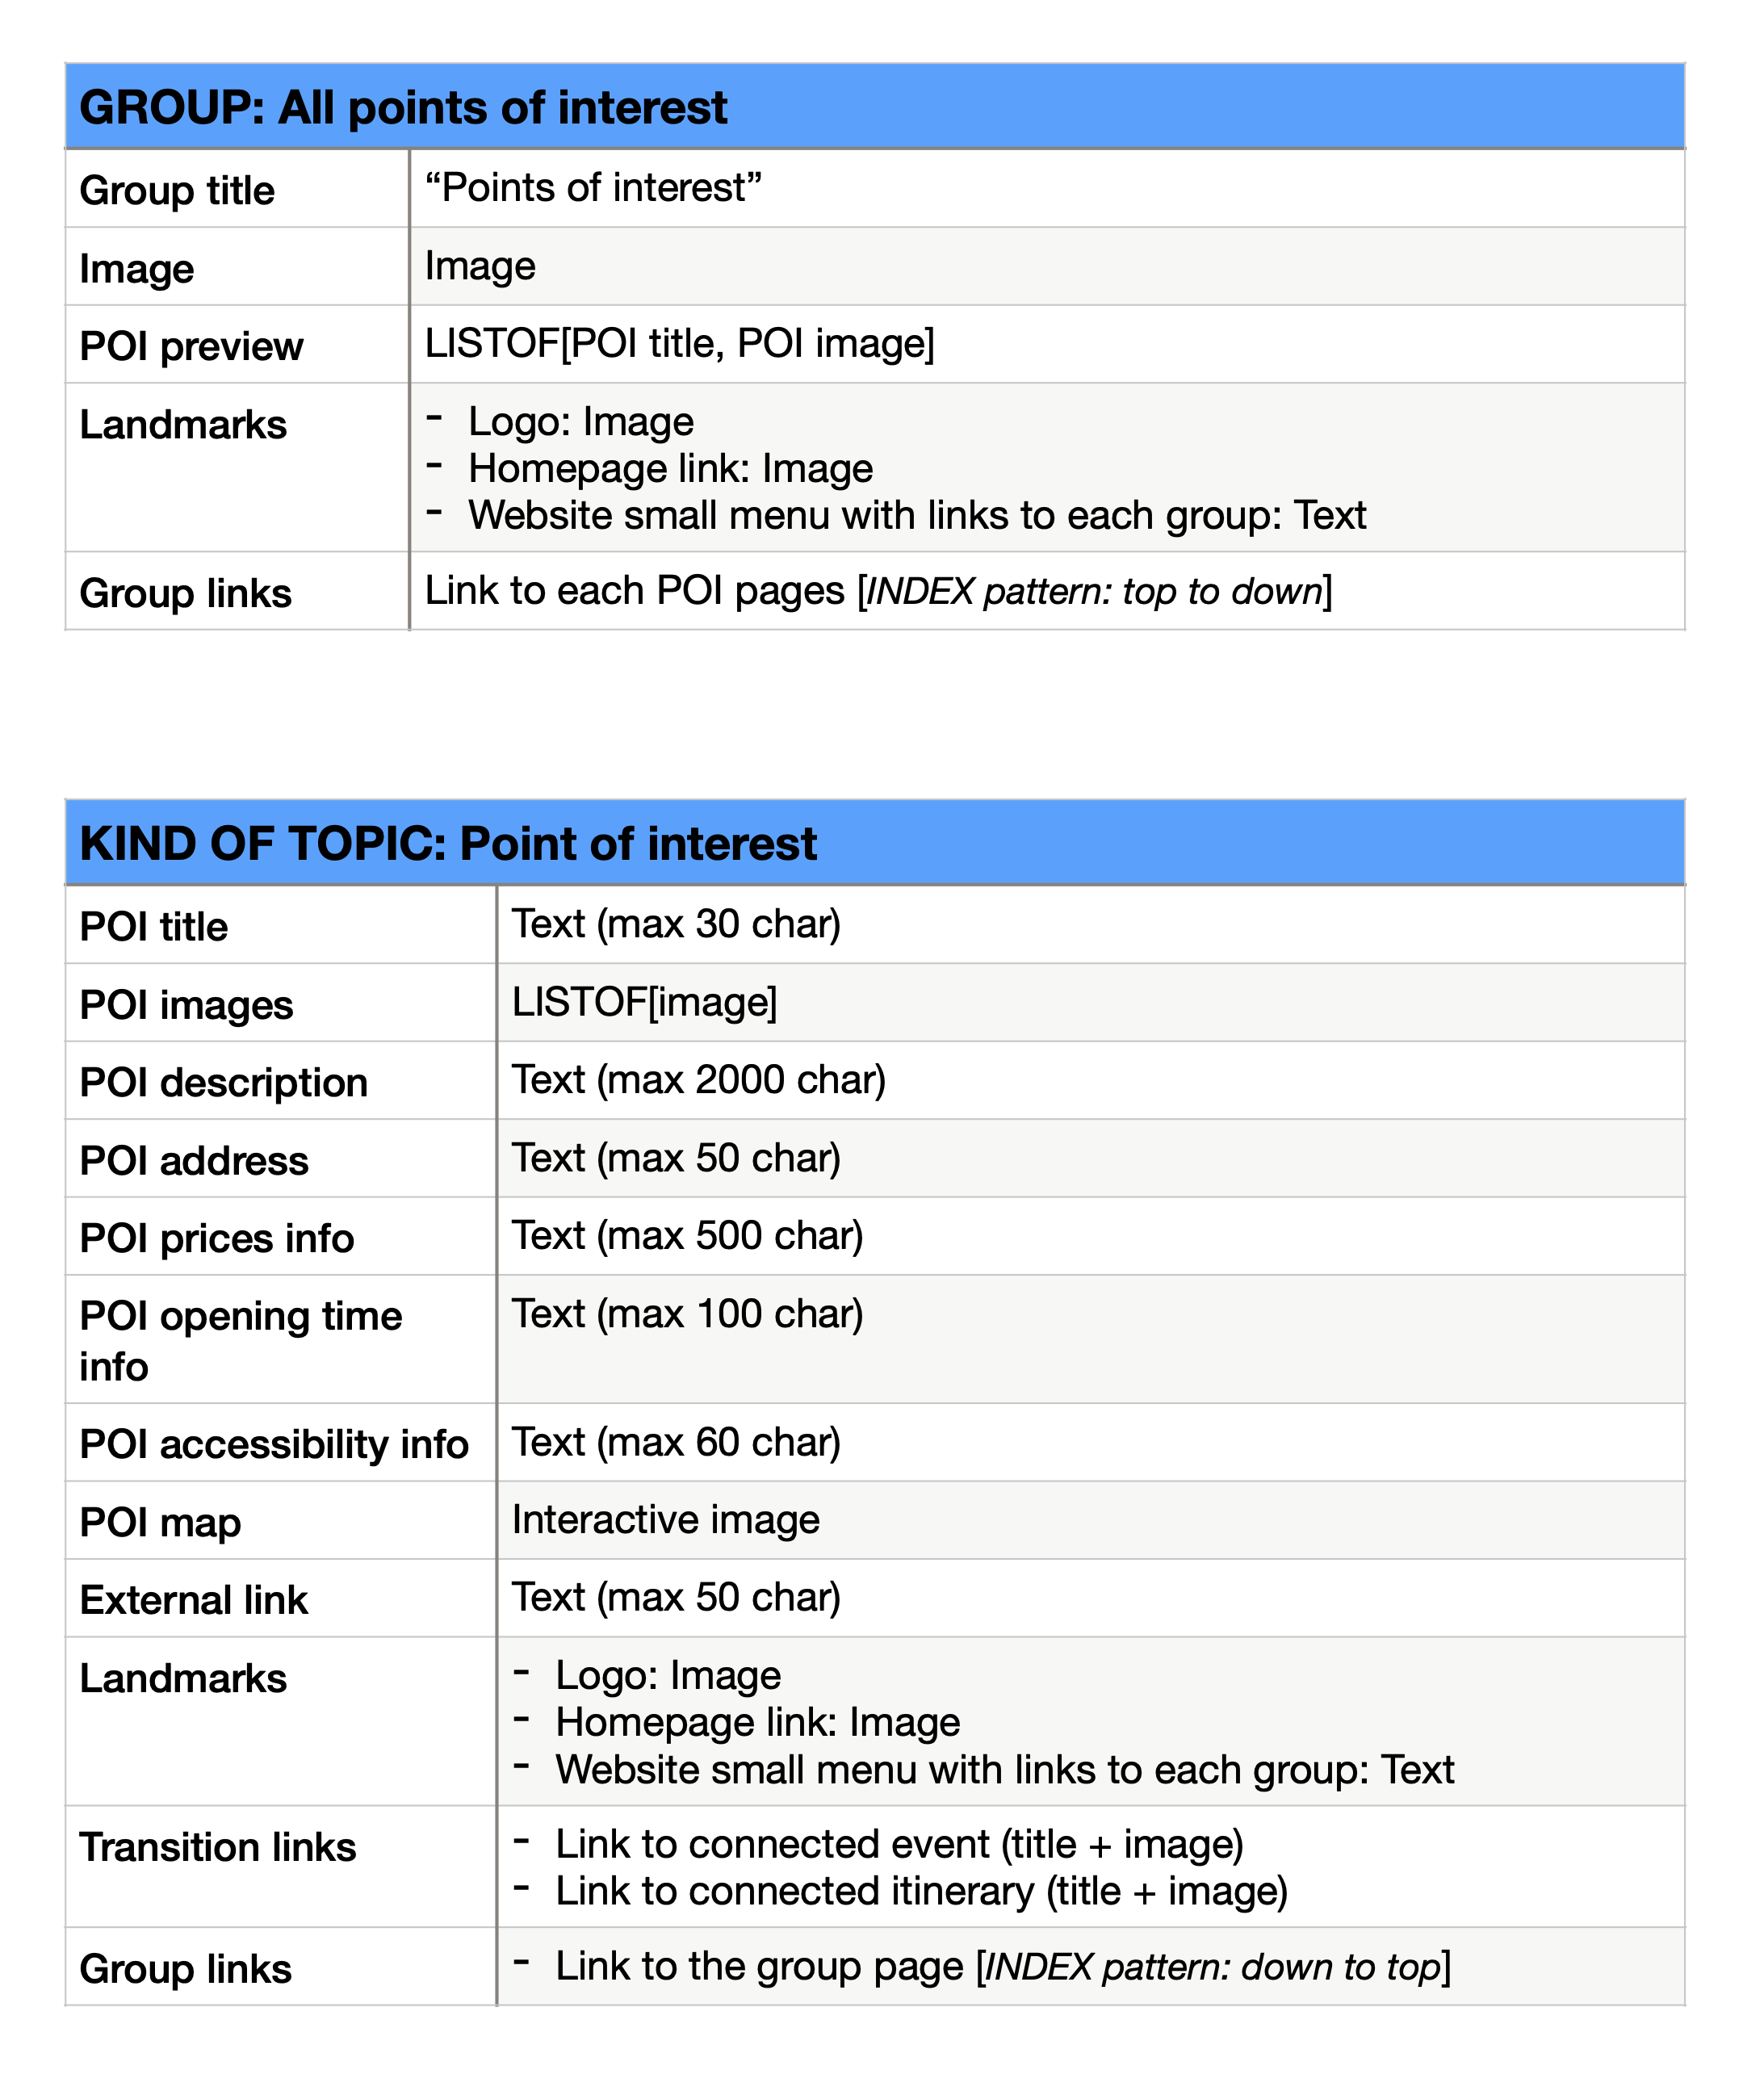
\includegraphics[width=\textwidth]{assets/Tables/Abstract/abstractPage2.png}
        \caption{Abstract pages}
    \end{center}
\end{figure}

\begin{figure}[H]
    \begin{center}
        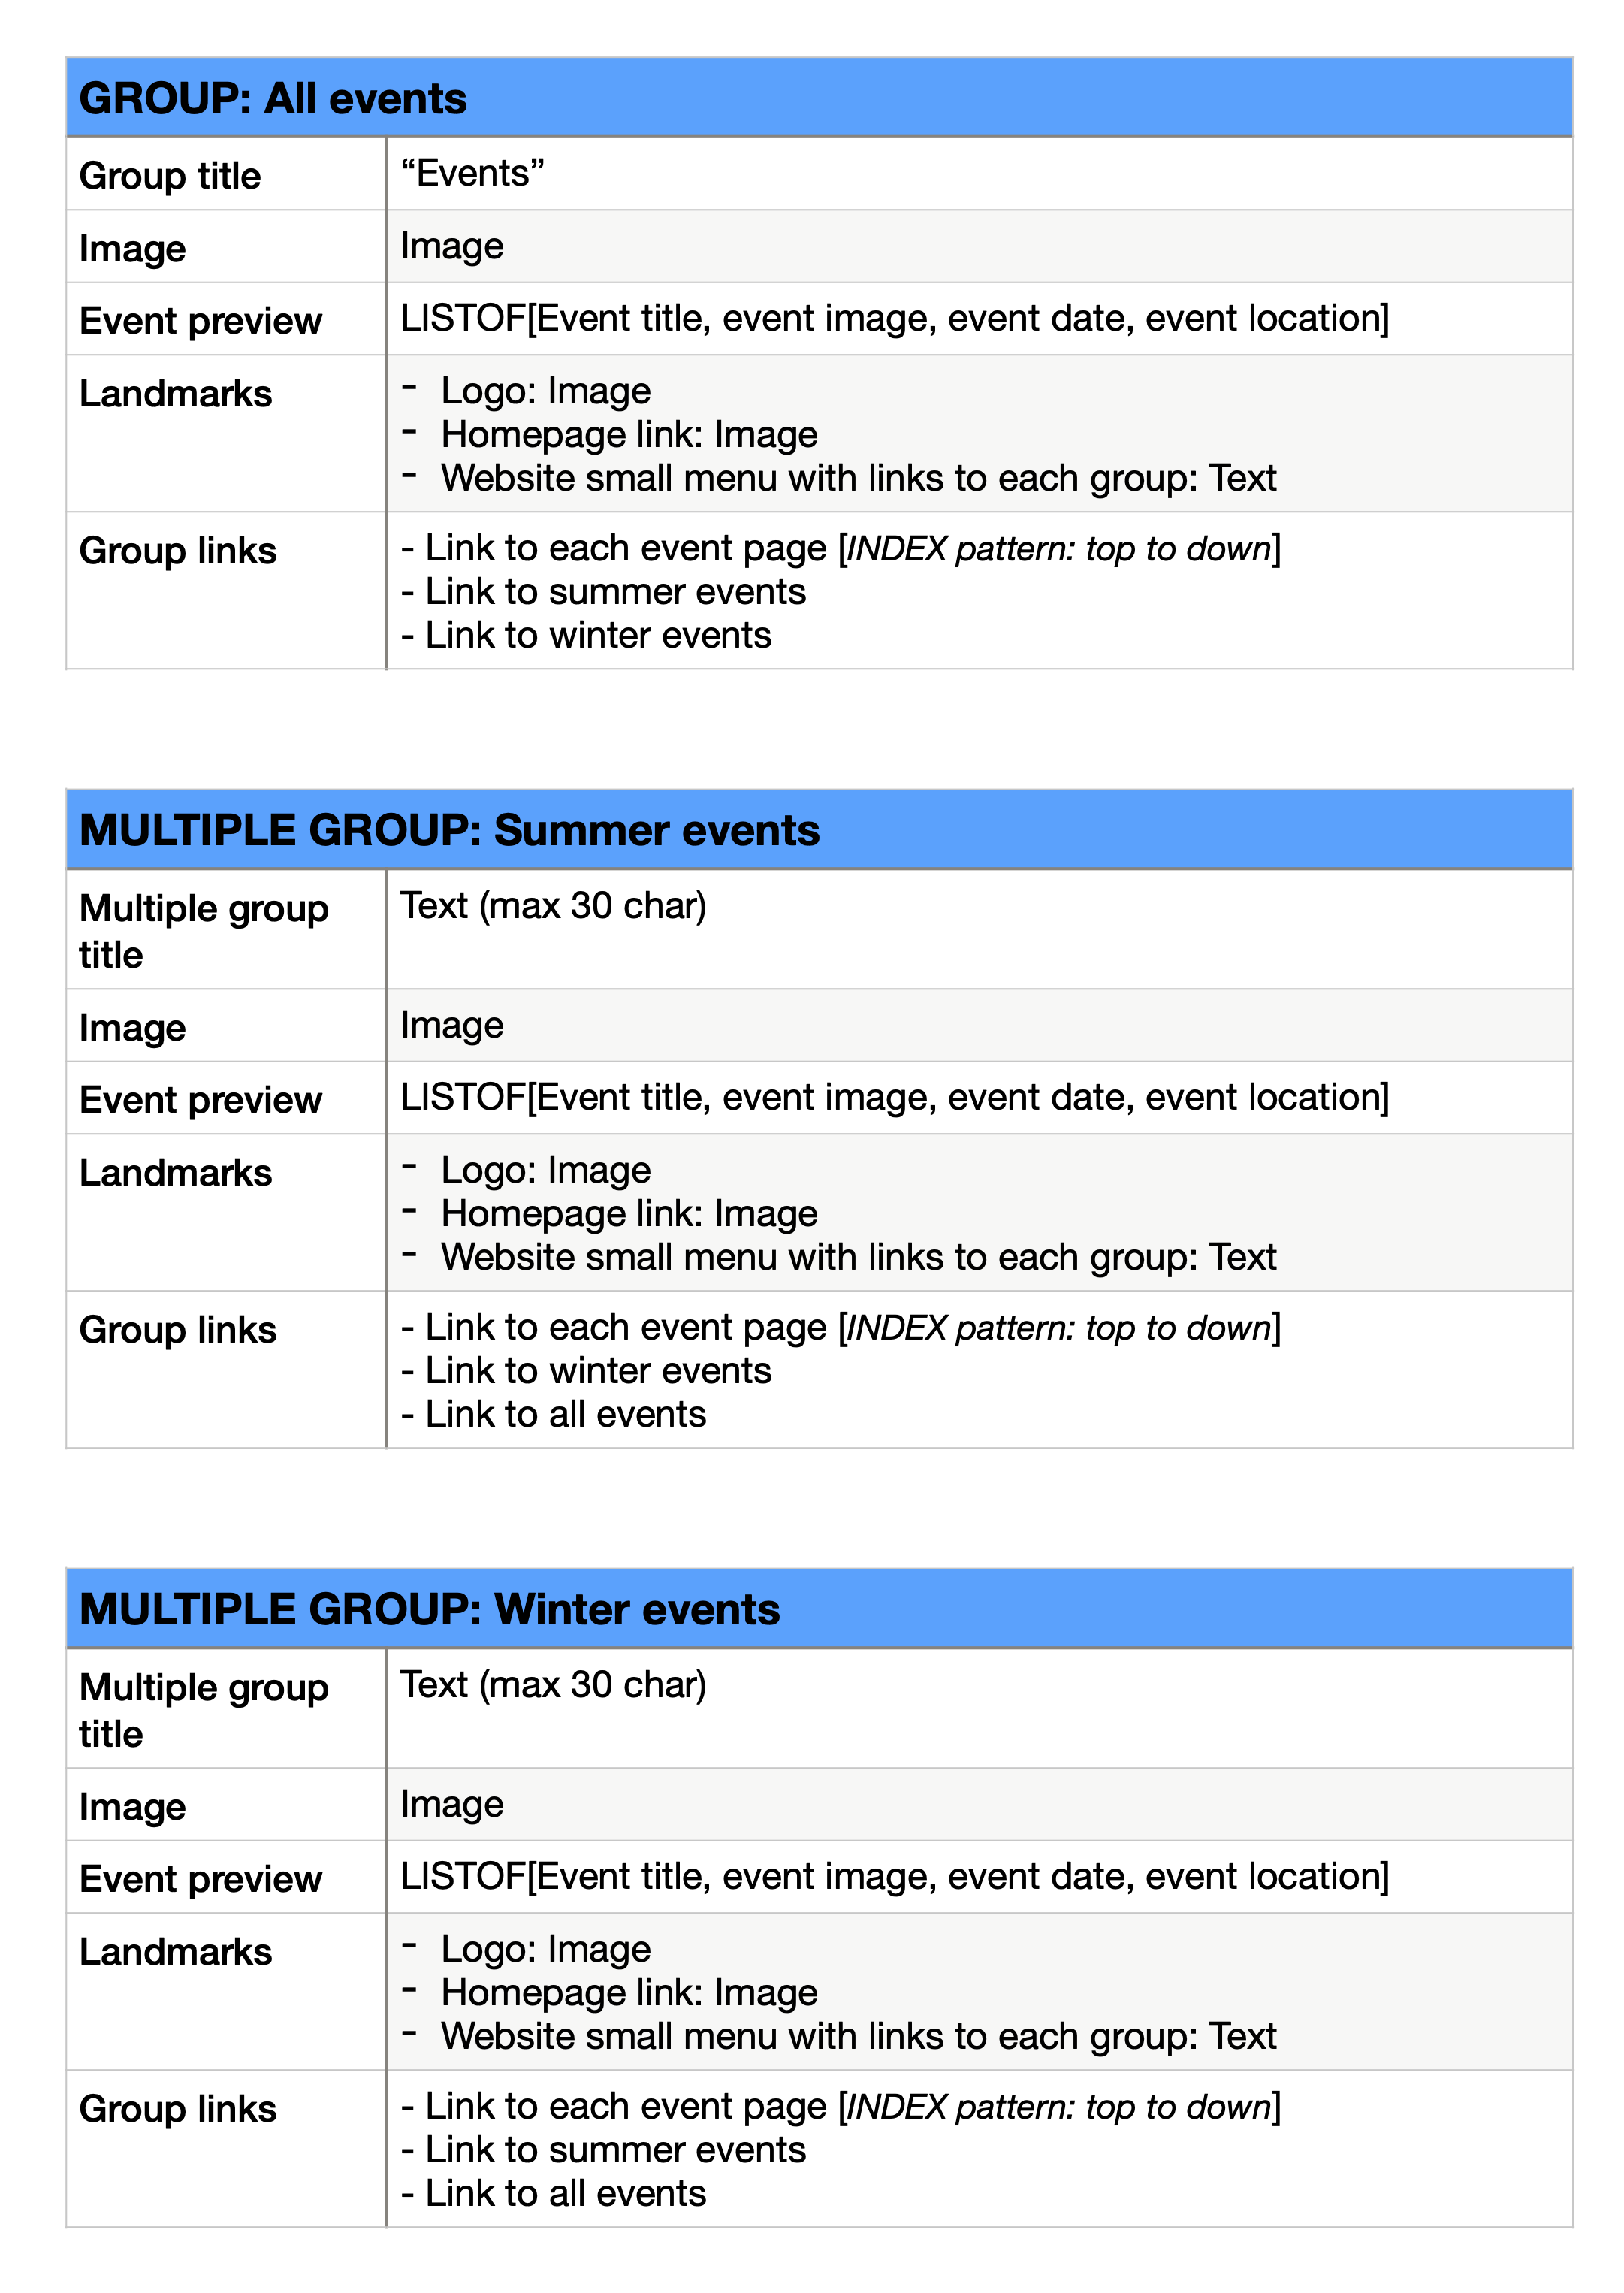
\includegraphics[width=\textwidth]{assets/Tables/Abstract/abstractPage3.png}
        \caption{Abstract pages}
    \end{center}
\end{figure}

\begin{figure}[H]
    \begin{center}
        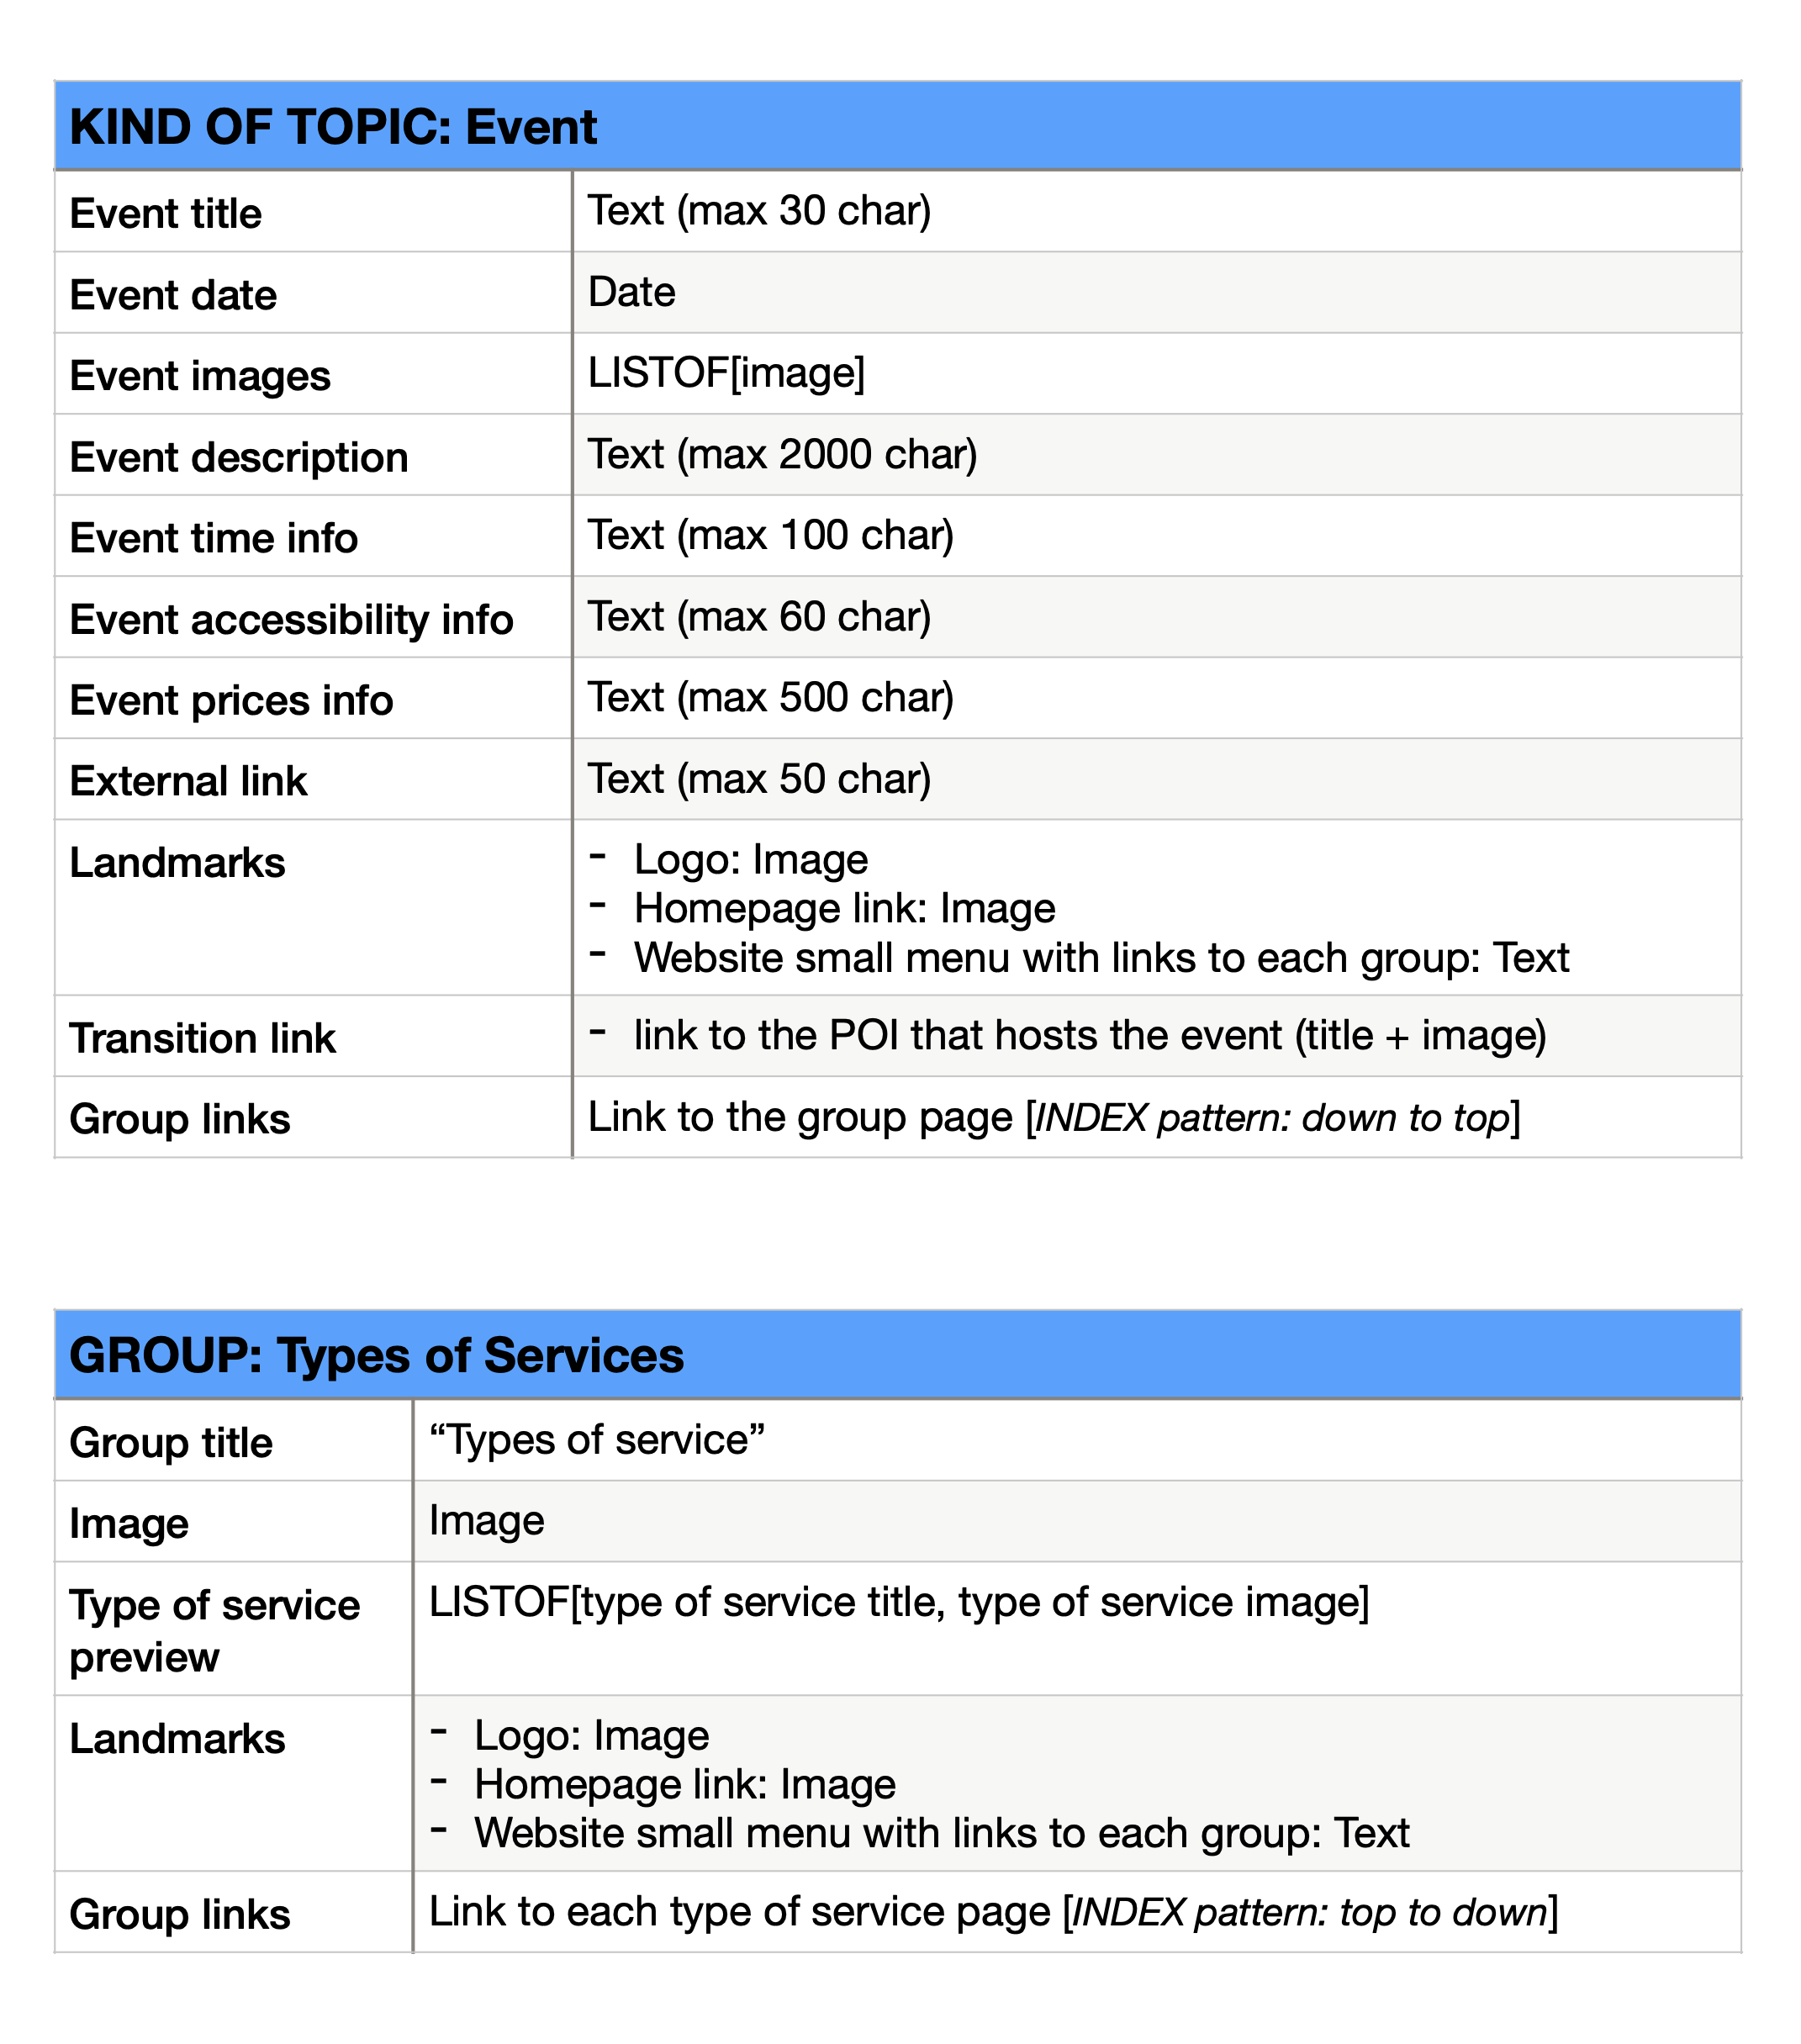
\includegraphics[width=\textwidth]{assets/Tables/Abstract/abstractPage4.png}
        \caption{Abstract pages}
    \end{center}
\end{figure}

\begin{figure}[H]
    \begin{center}
        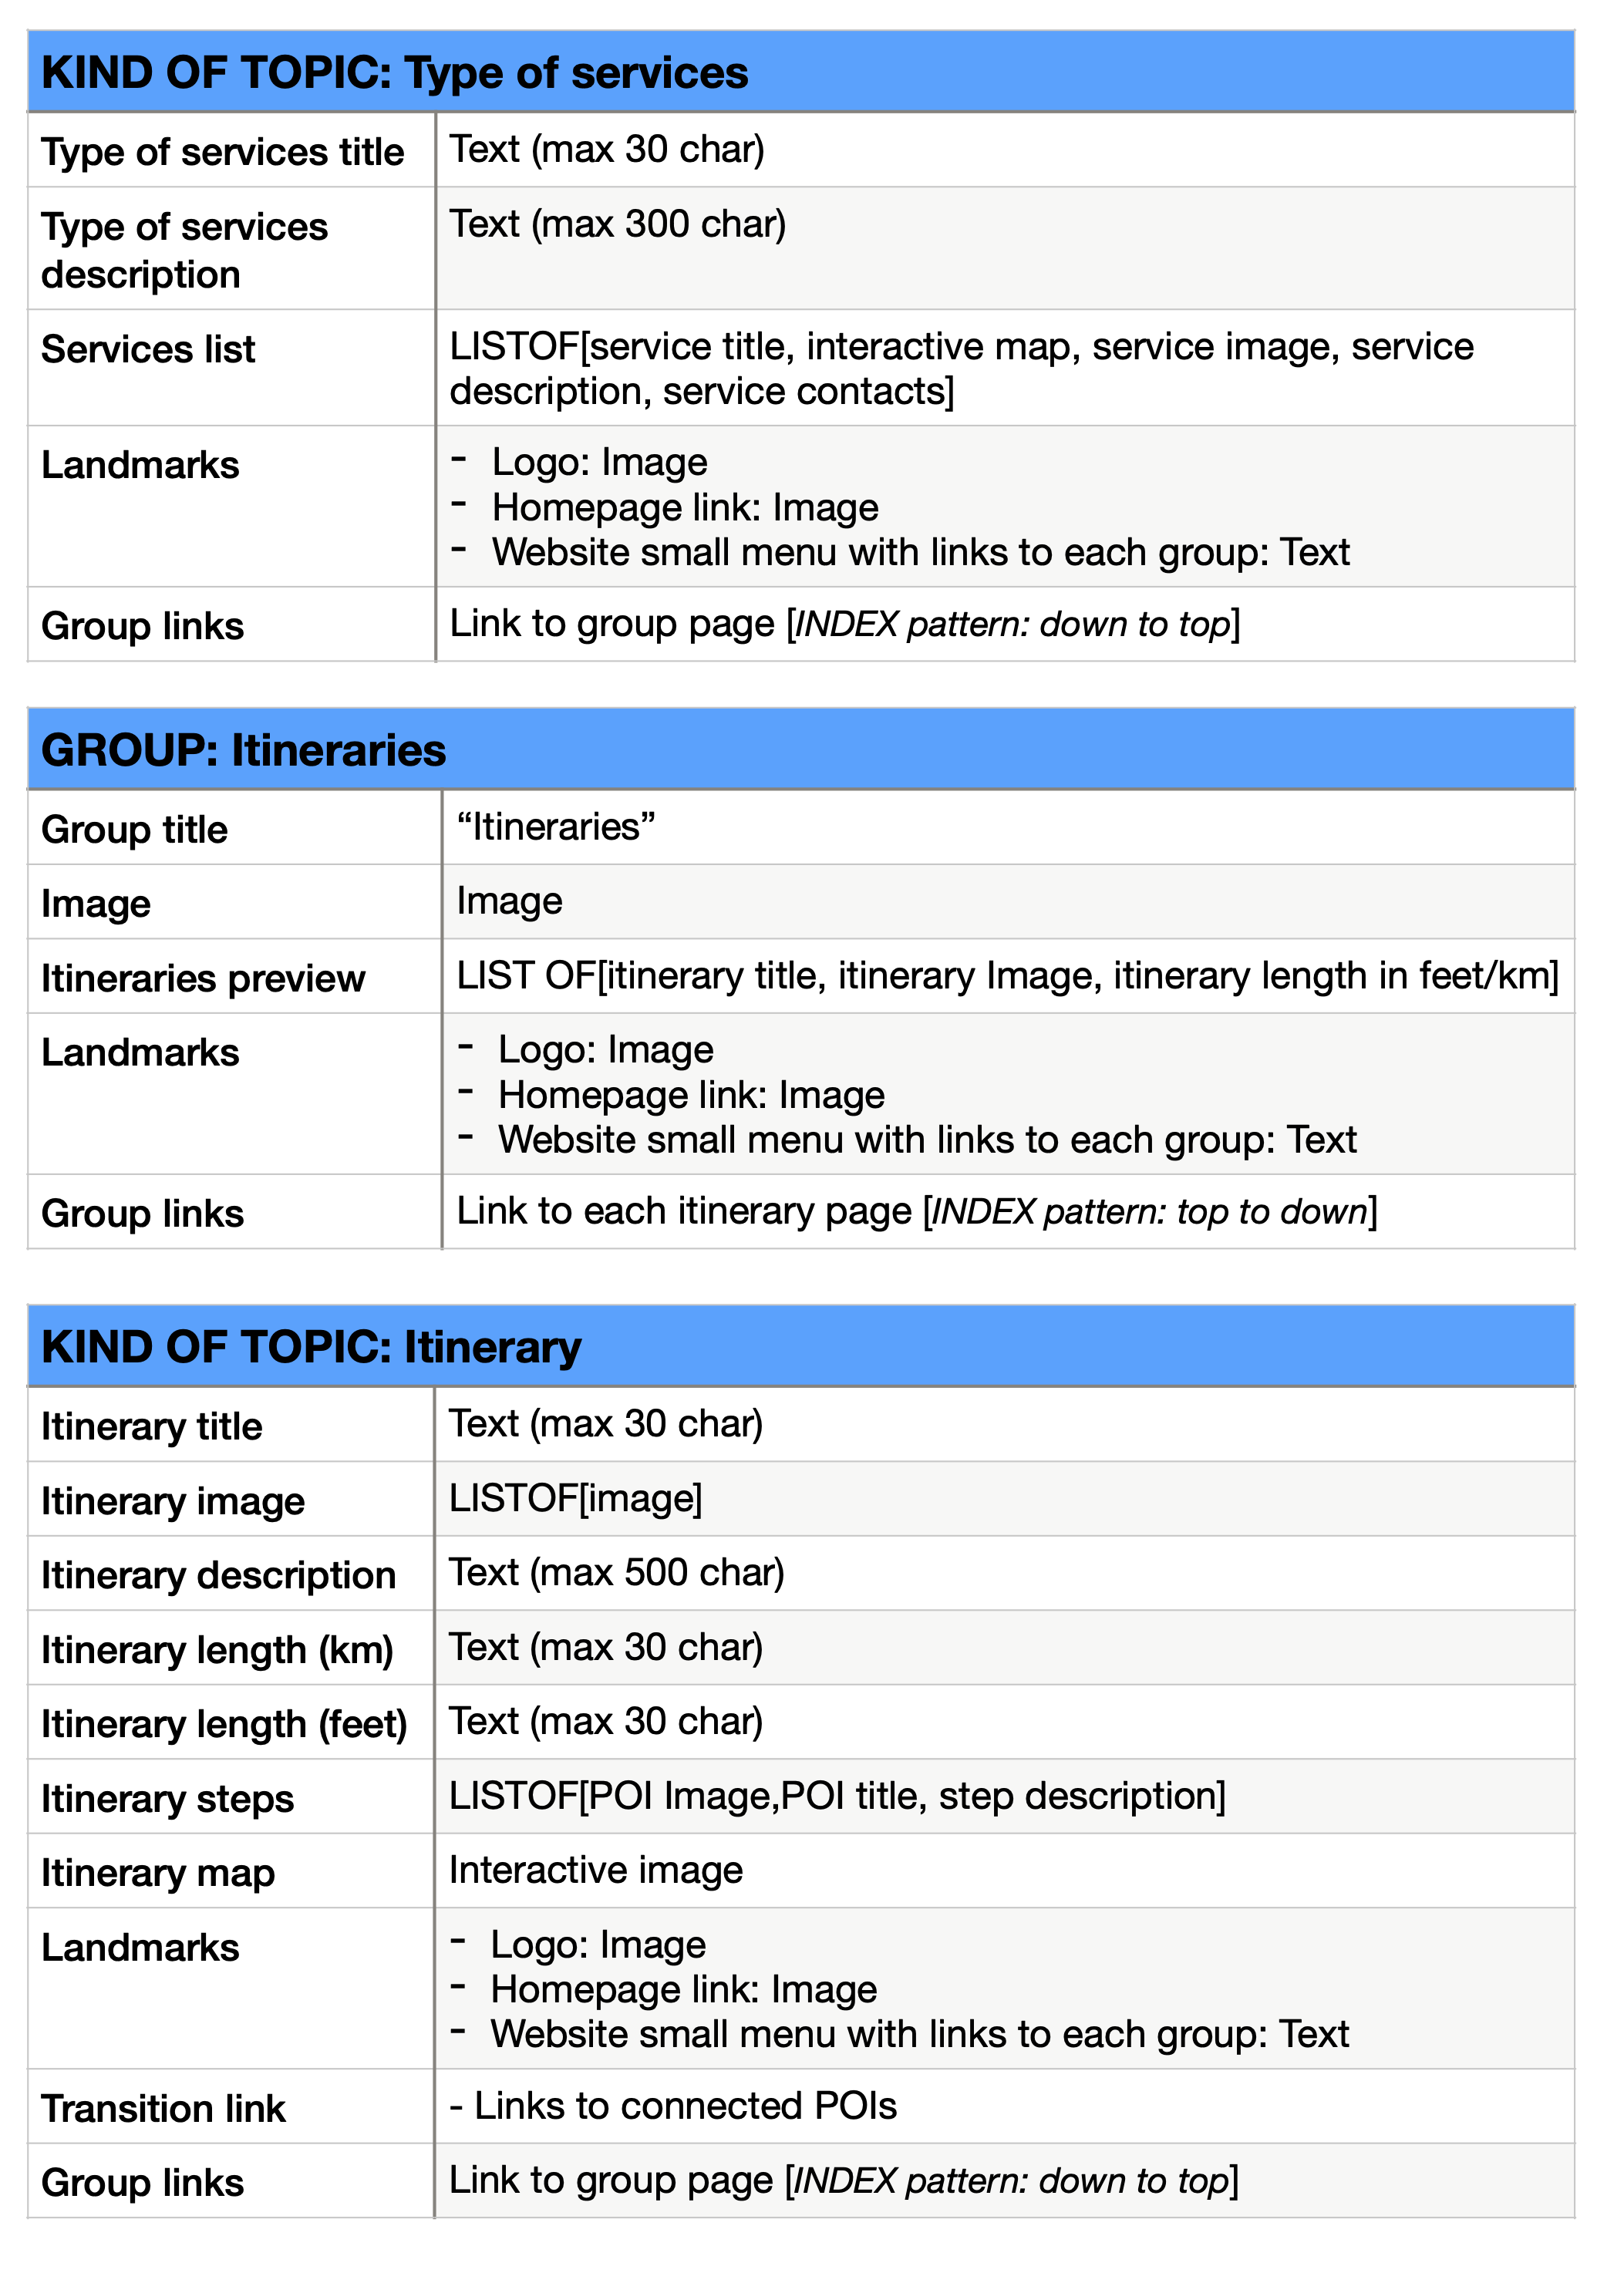
\includegraphics[width=\textwidth]{assets/Tables/Abstract/abstractPage5.png}
        \caption{Abstract pages}
    \end{center}
\end{figure}

\section{Website wireframes}
In this section screenshots of the webpage are showed with some comments, in order to have a coherence and reference with respect to the abstract pages tables.
\begin{figure}[H]
    \begin{center}
        \includegraphics[width=\textwidth]{assets/Wireframes/homepage.png}
        \caption{Homepage wireframe}
    \end{center}
\end{figure}

\begin{figure}[H]
    \begin{center}
        \includegraphics[width=\textwidth]{assets/Wireframes/about.png}
        \caption{About wireframe}
    \end{center}
\end{figure}

\begin{figure}[H]
    \begin{center}
        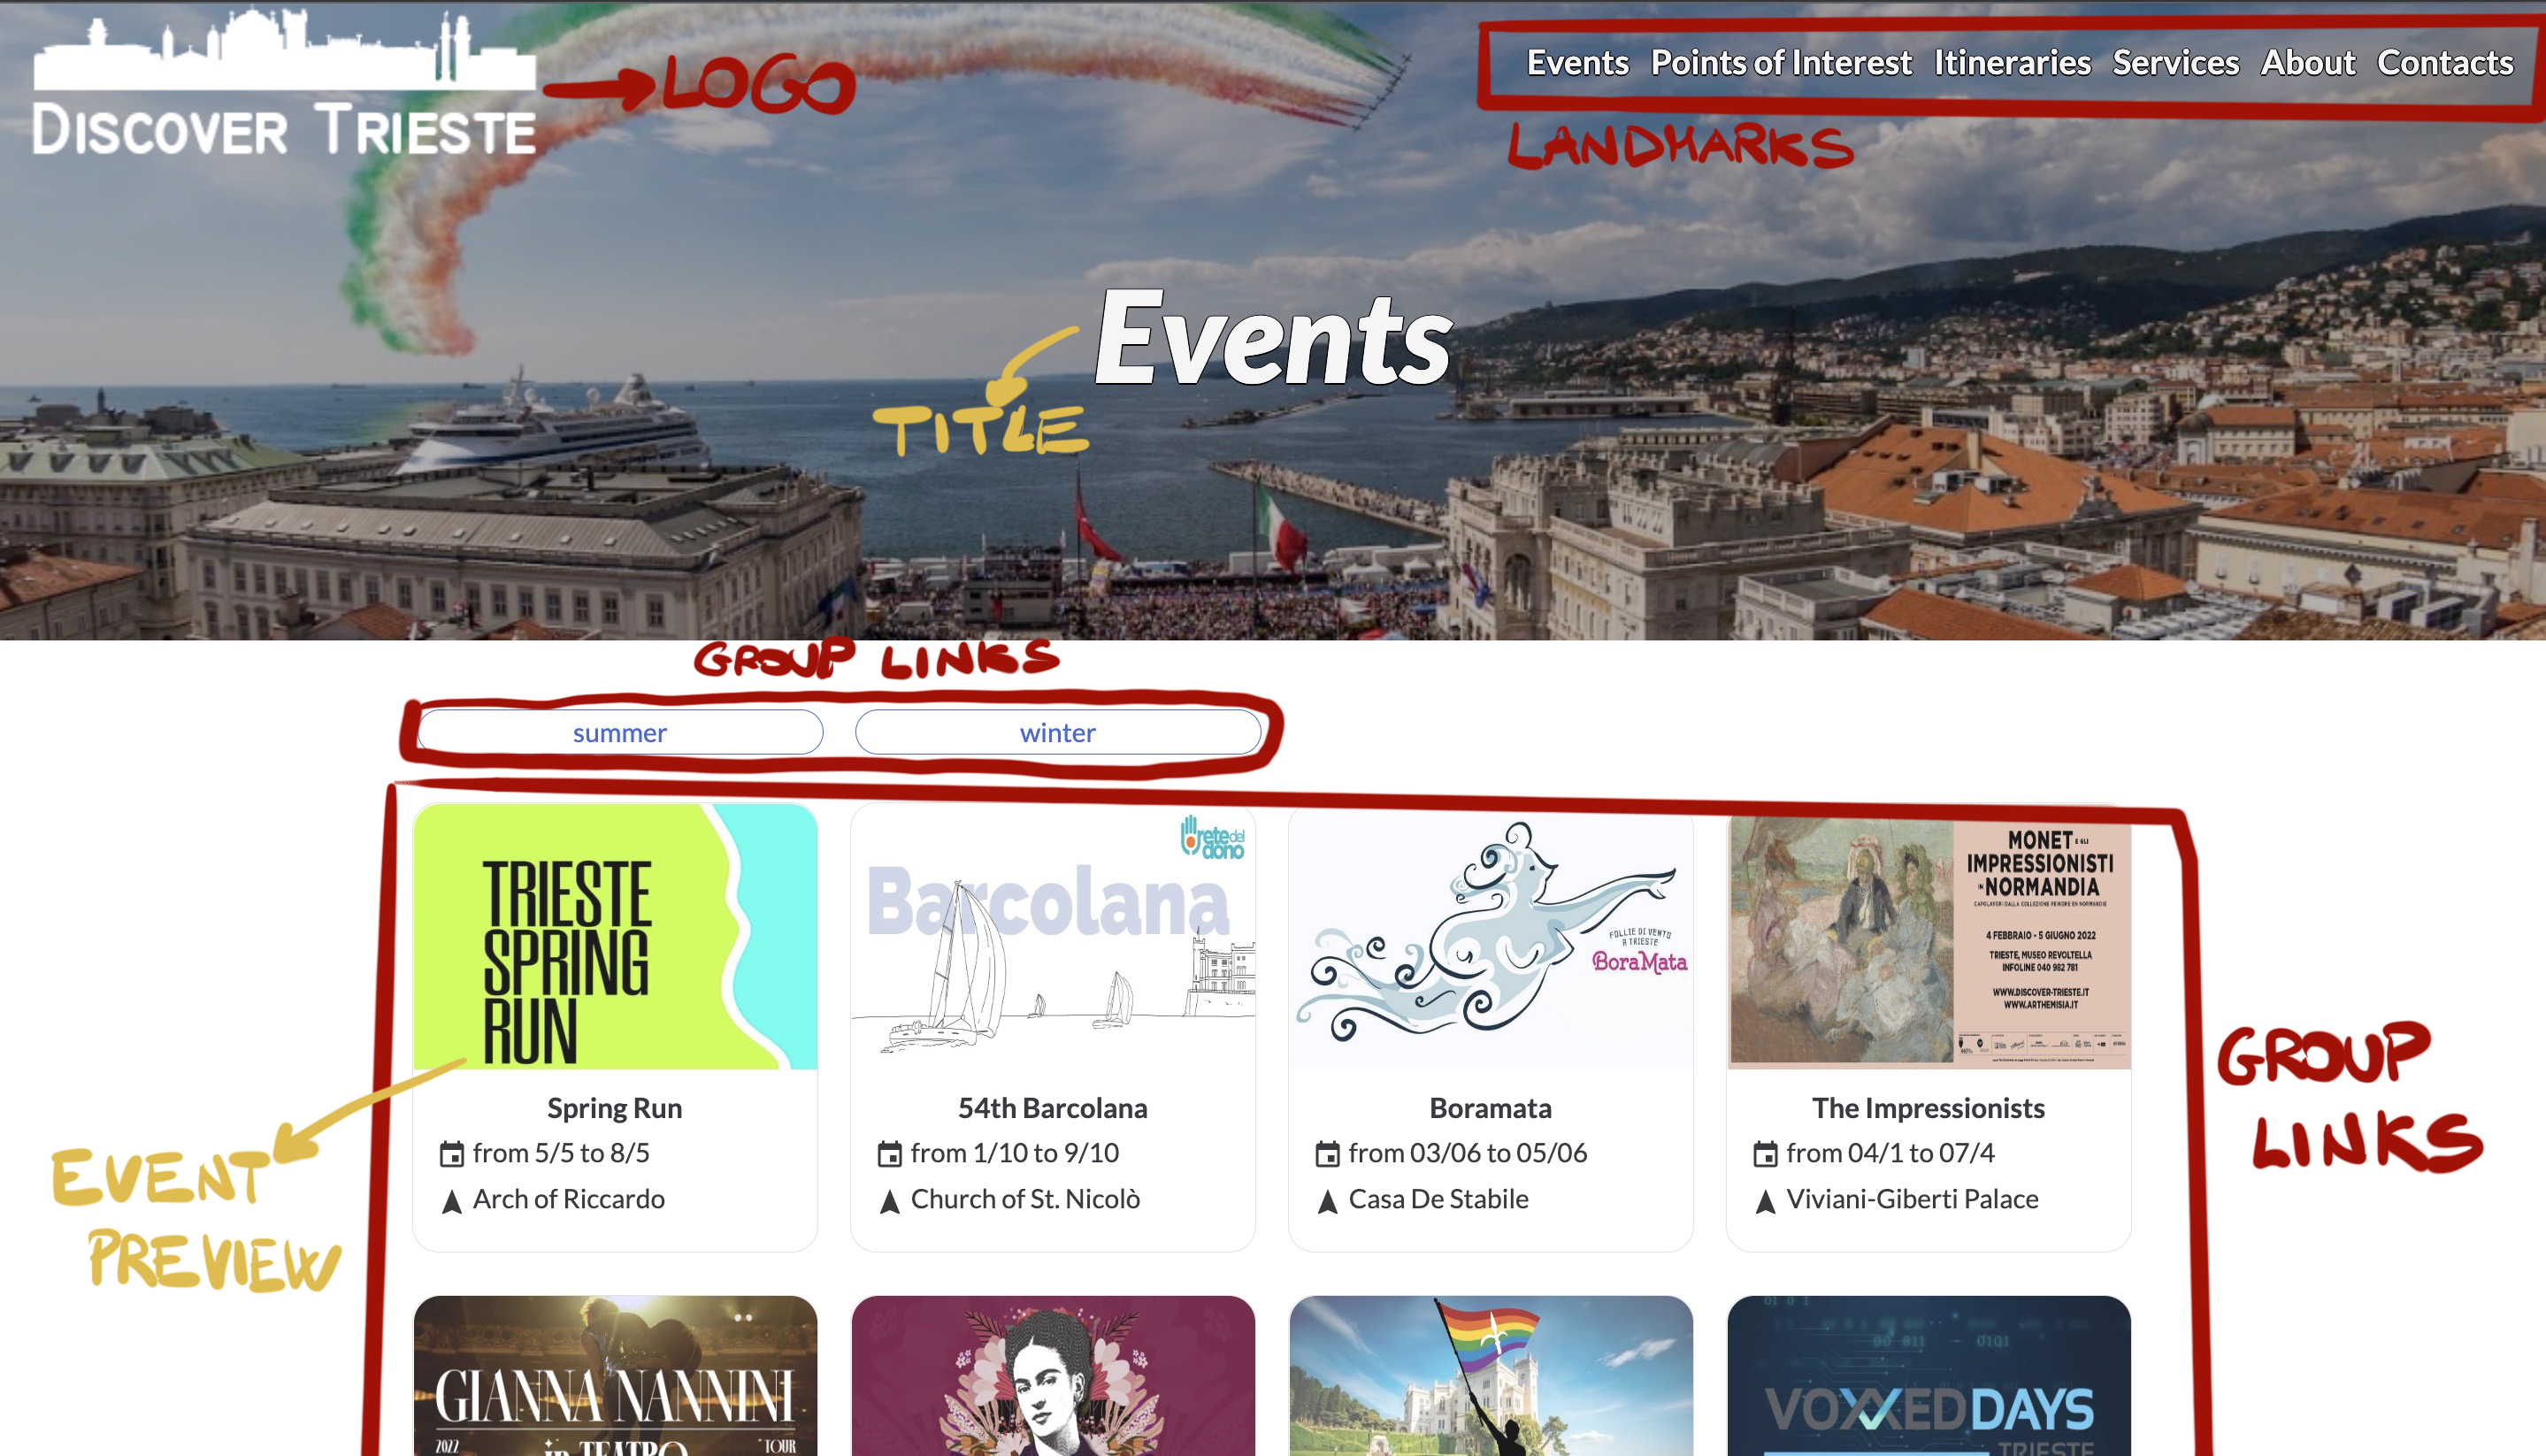
\includegraphics[width=\textwidth]{assets/Wireframes/allEvents.png}
        \caption{Event (group of topic) wireframe}
    \end{center}
\end{figure}

\begin{figure}[H]
    \begin{center}
        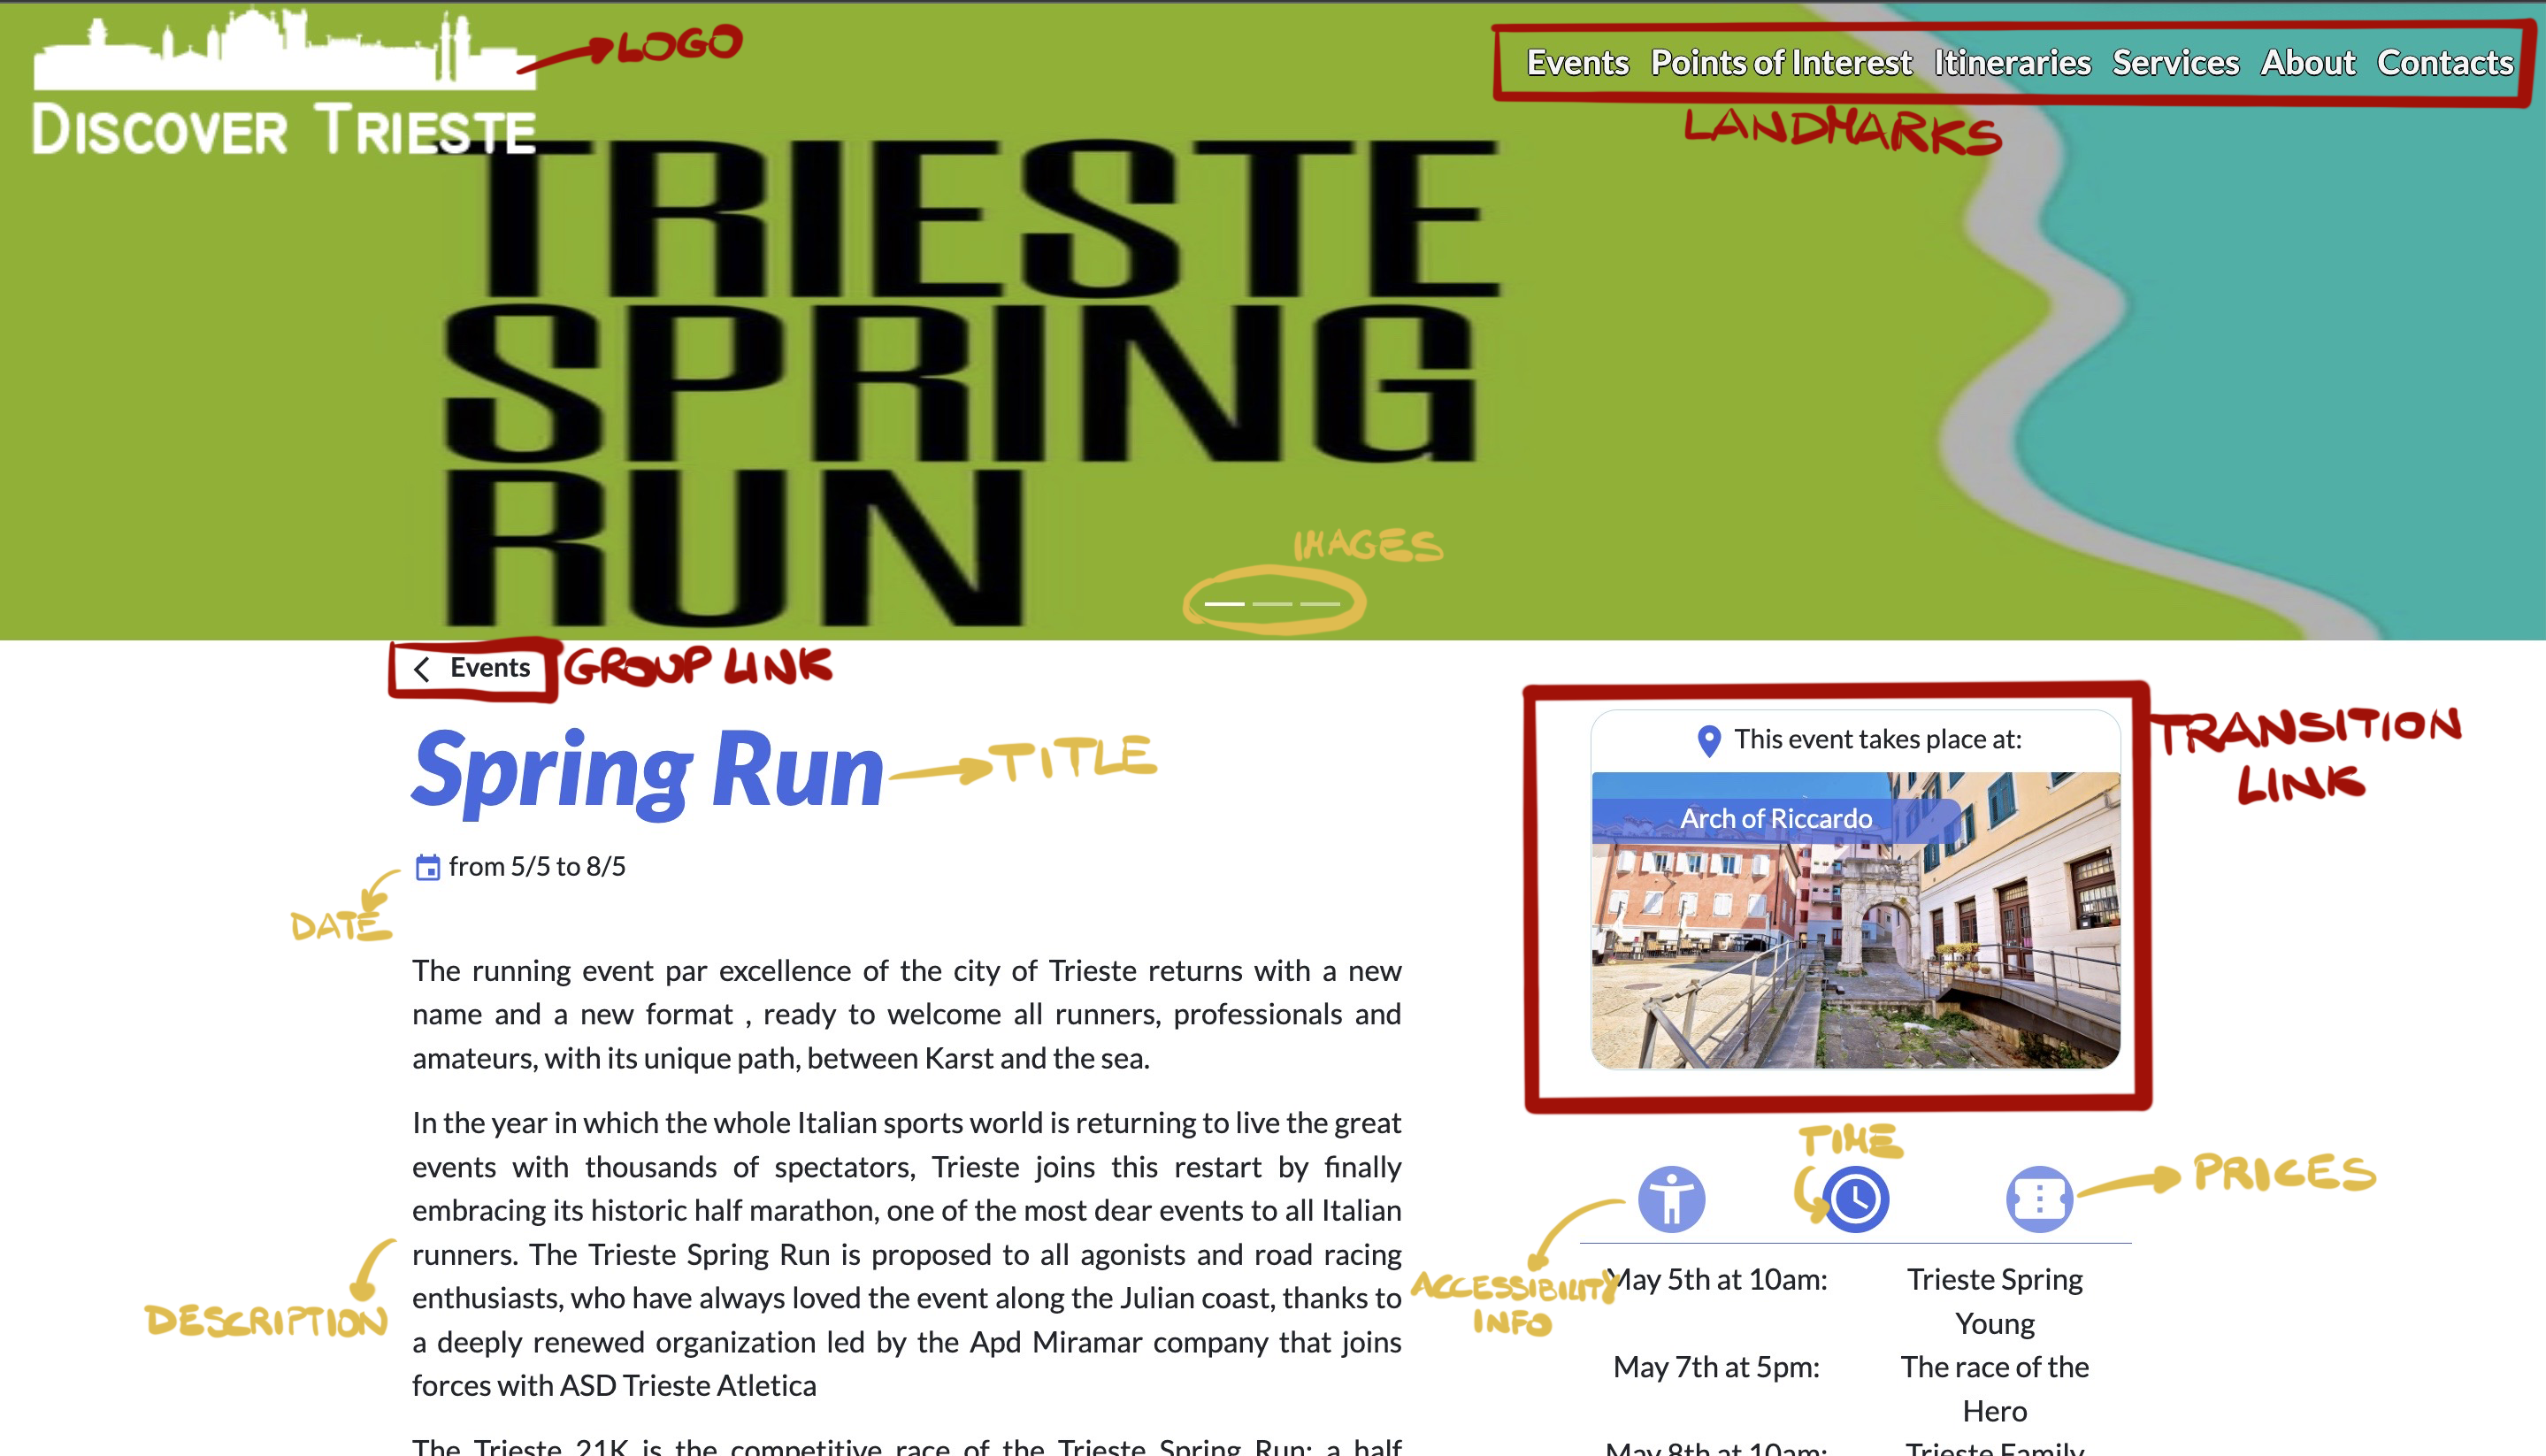
\includegraphics[width=\textwidth]{assets/Wireframes/event.png}
        \caption{Event (kind of topic) wireframe}
    \end{center}
\end{figure}

\begin{figure}[H]
    \begin{center}
        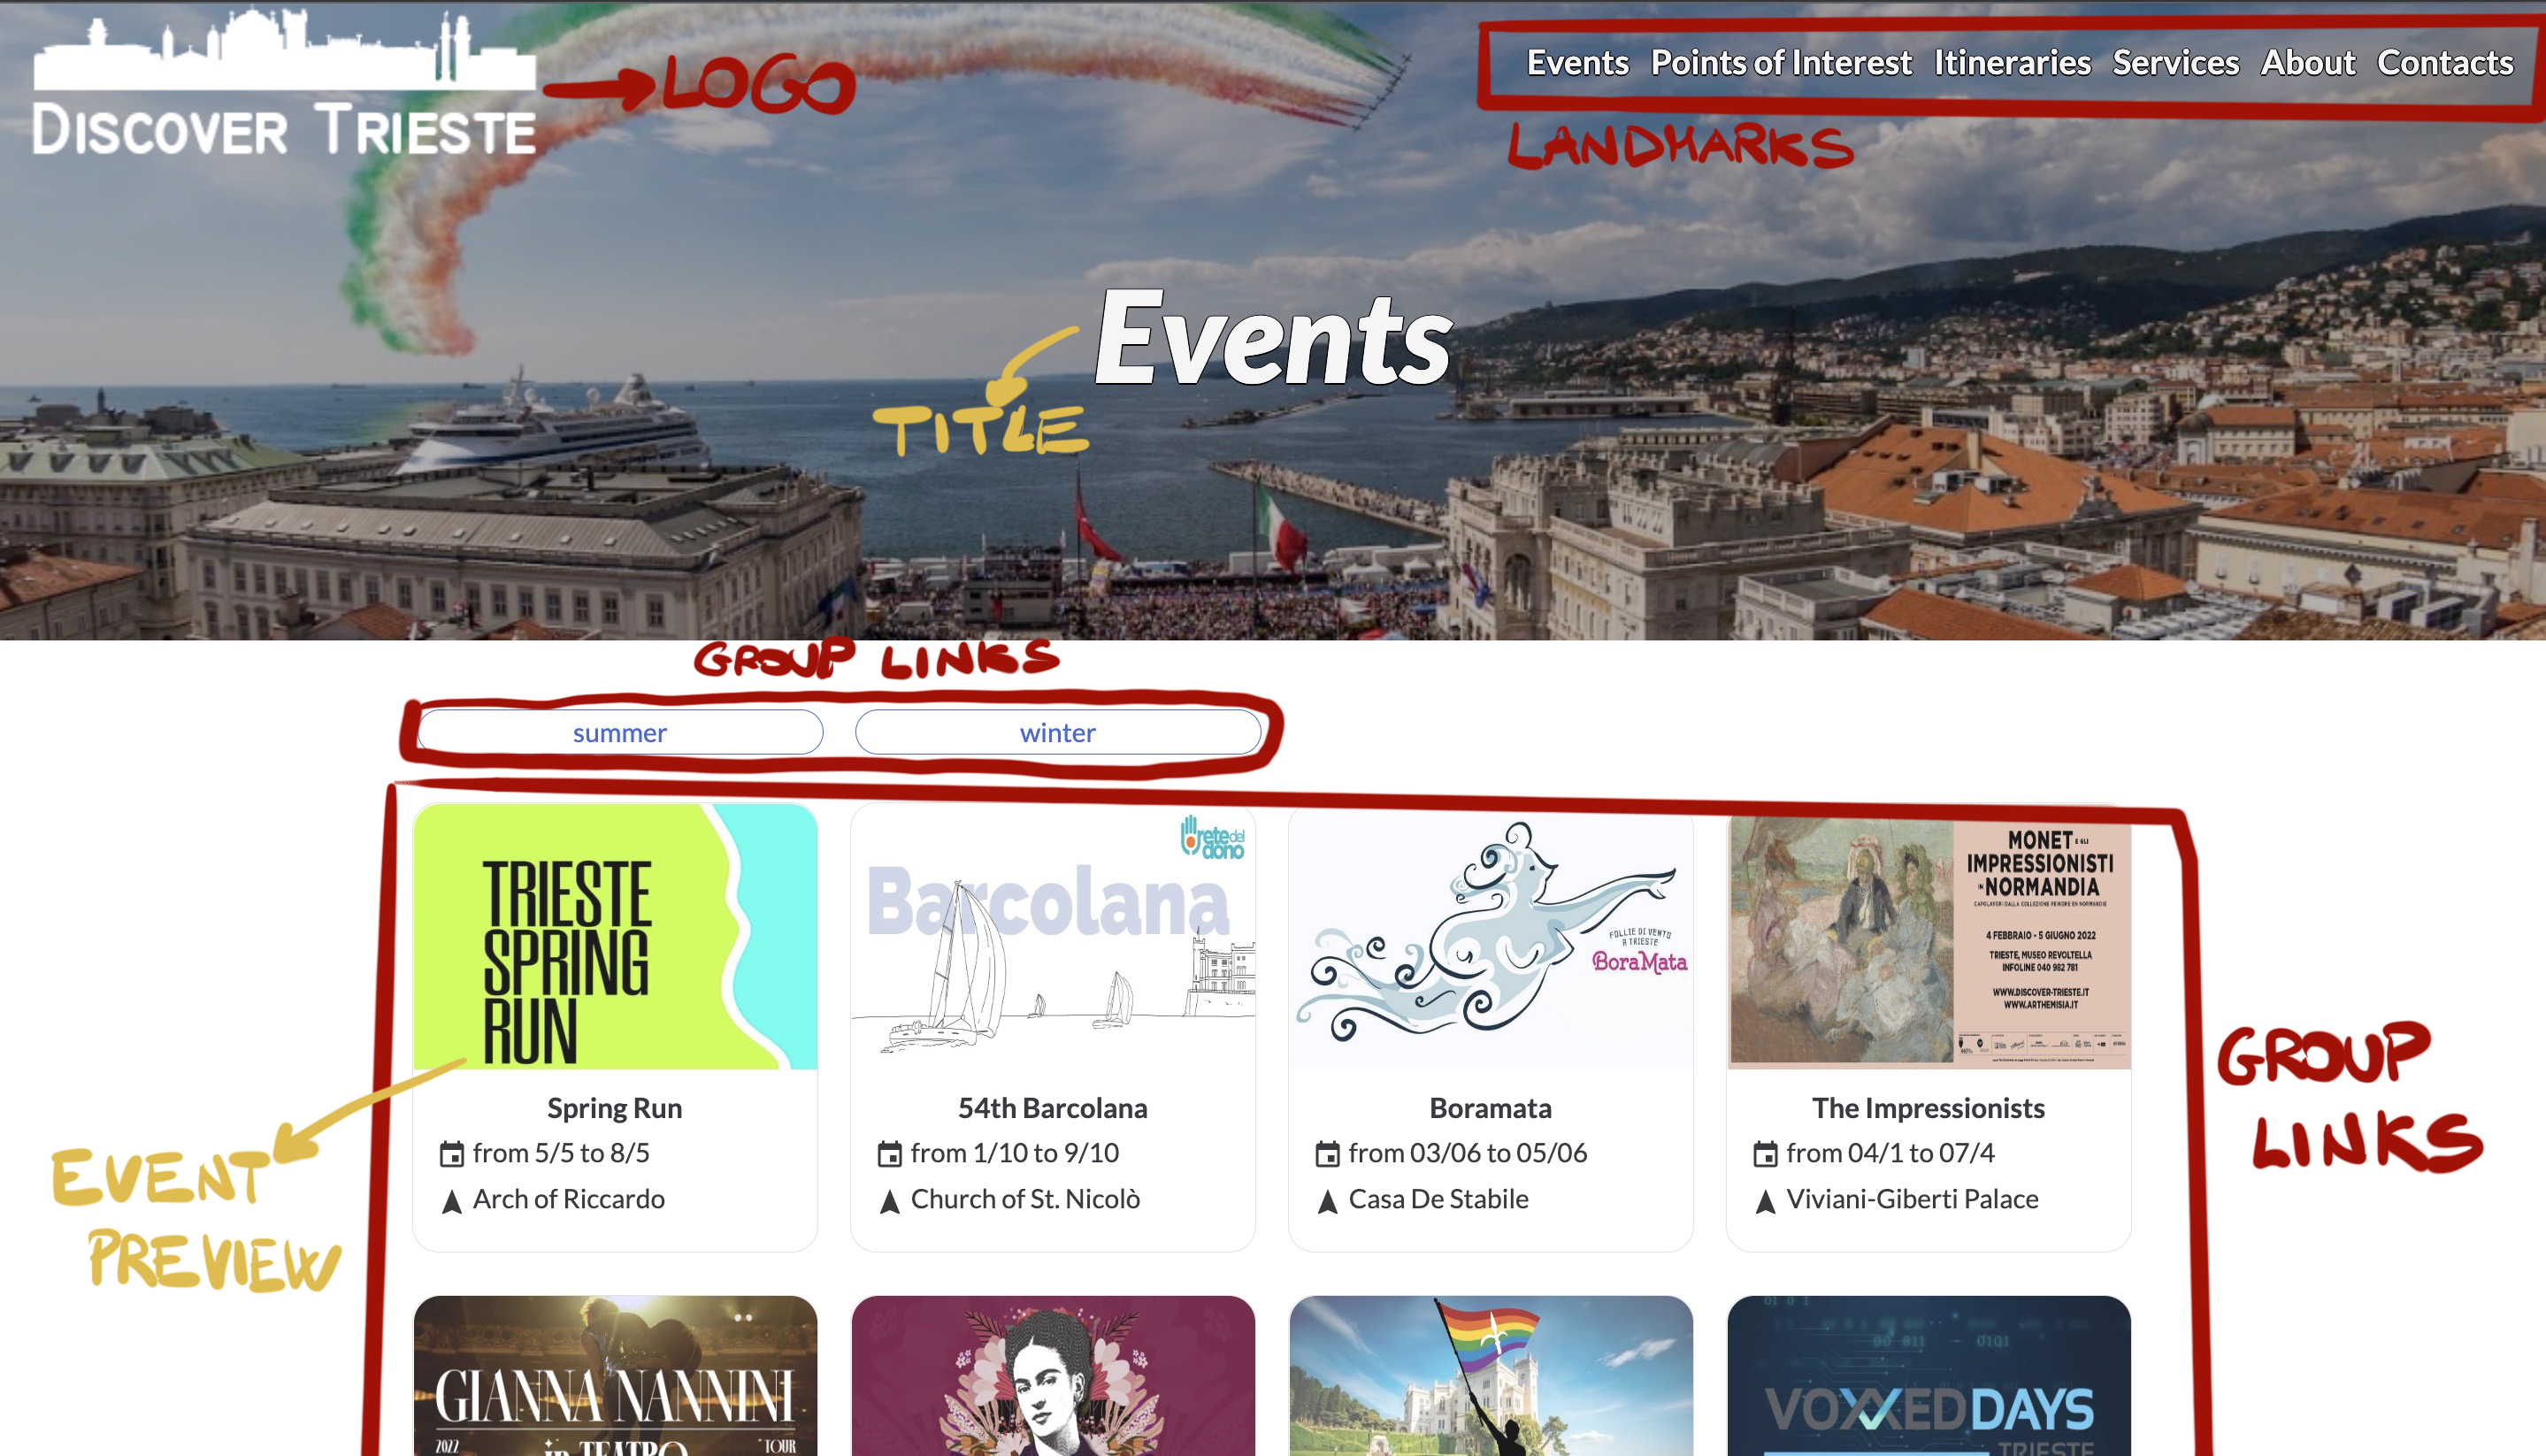
\includegraphics[width=\textwidth]{assets/Wireframes/allEvents.png}
        \caption{Itinerary (group of topic) wireframe}
    \end{center}
\end{figure}

\begin{figure}[H]
    \begin{center}
        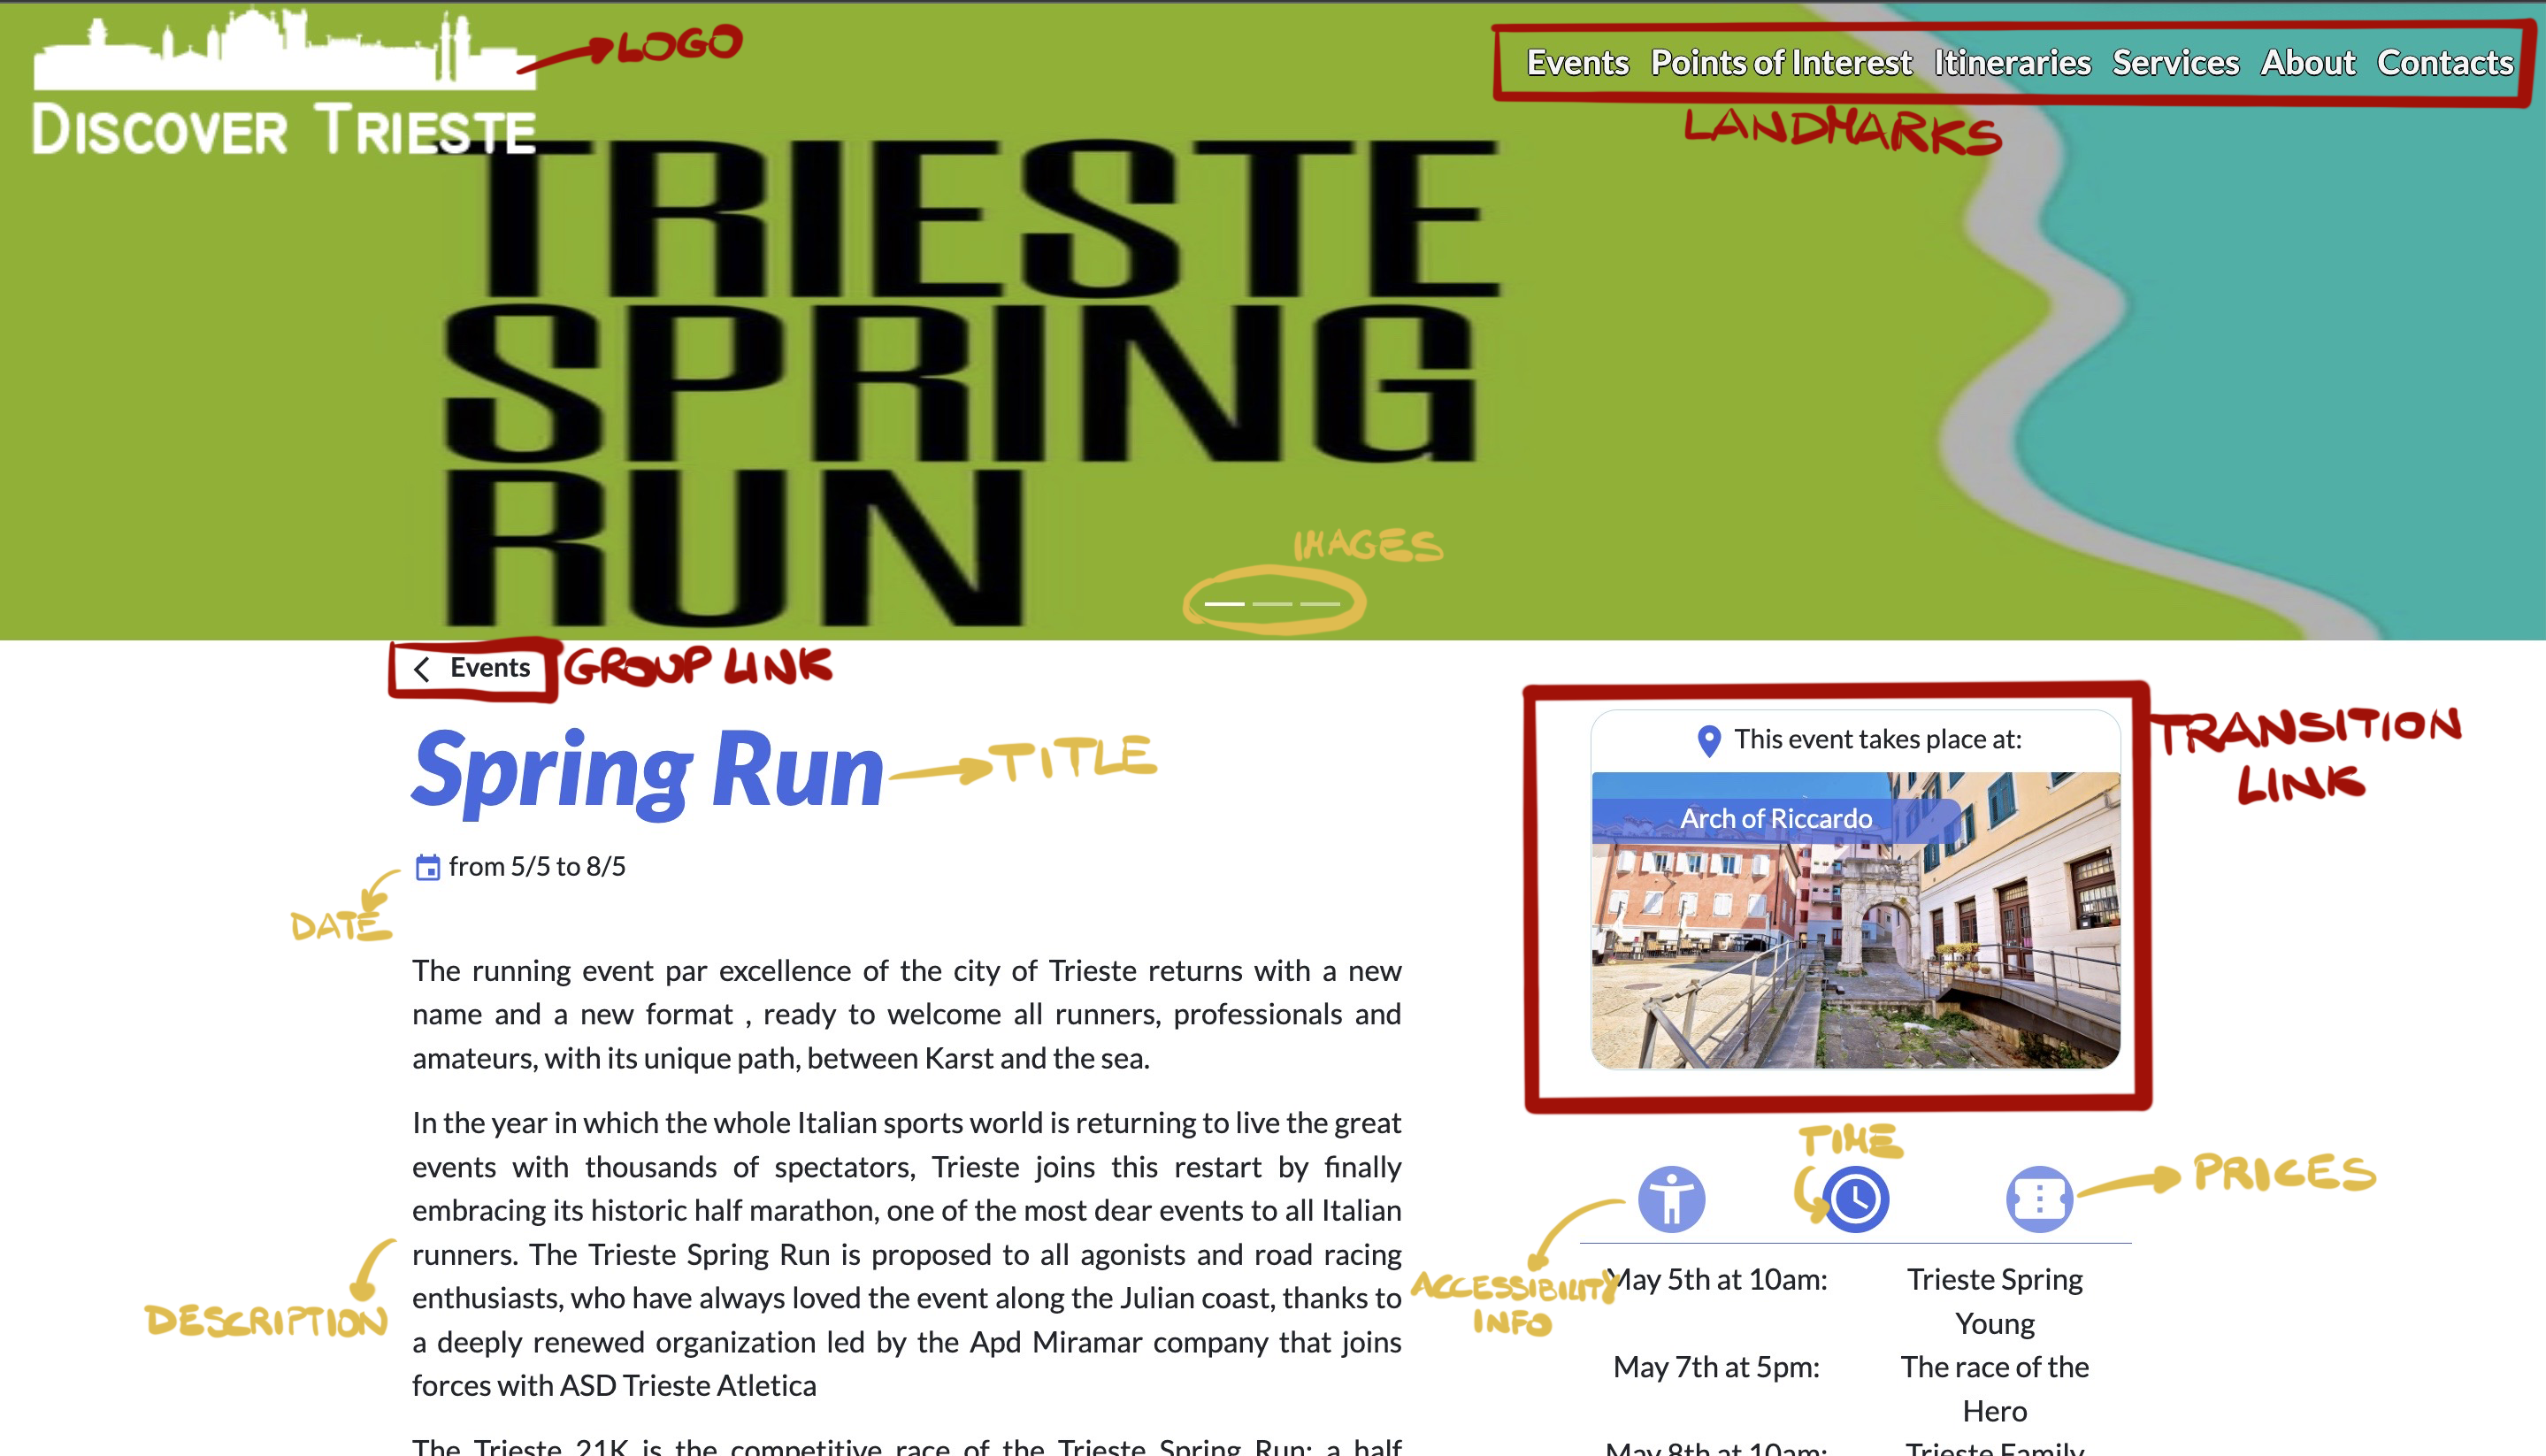
\includegraphics[width=\textwidth]{assets/Wireframes/event.png}
        \caption{Itinerary (kind of topic) wireframe}
    \end{center}
\end{figure}

\begin{figure}[H]
    \begin{center}
        \includegraphics[width=\textwidth]{assets/Wireframes/allPois.png}
        \caption{Point of interest (group of topic) wireframe}
    \end{center}
\end{figure}

\begin{figure}[H]
    \begin{center}
        \includegraphics[width=\textwidth]{assets/Wireframes/poi.png}
        \caption{Point of interest (kind of topic) wireframe}
    \end{center}
\end{figure}

\begin{figure}[H]
    \begin{center}
        \includegraphics[width=\textwidth]{assets/Wireframes/typesService.png}
        \caption{Type of service (group of topic) wireframe}
    \end{center}
\end{figure}

\begin{figure}[H]
    \begin{center}
        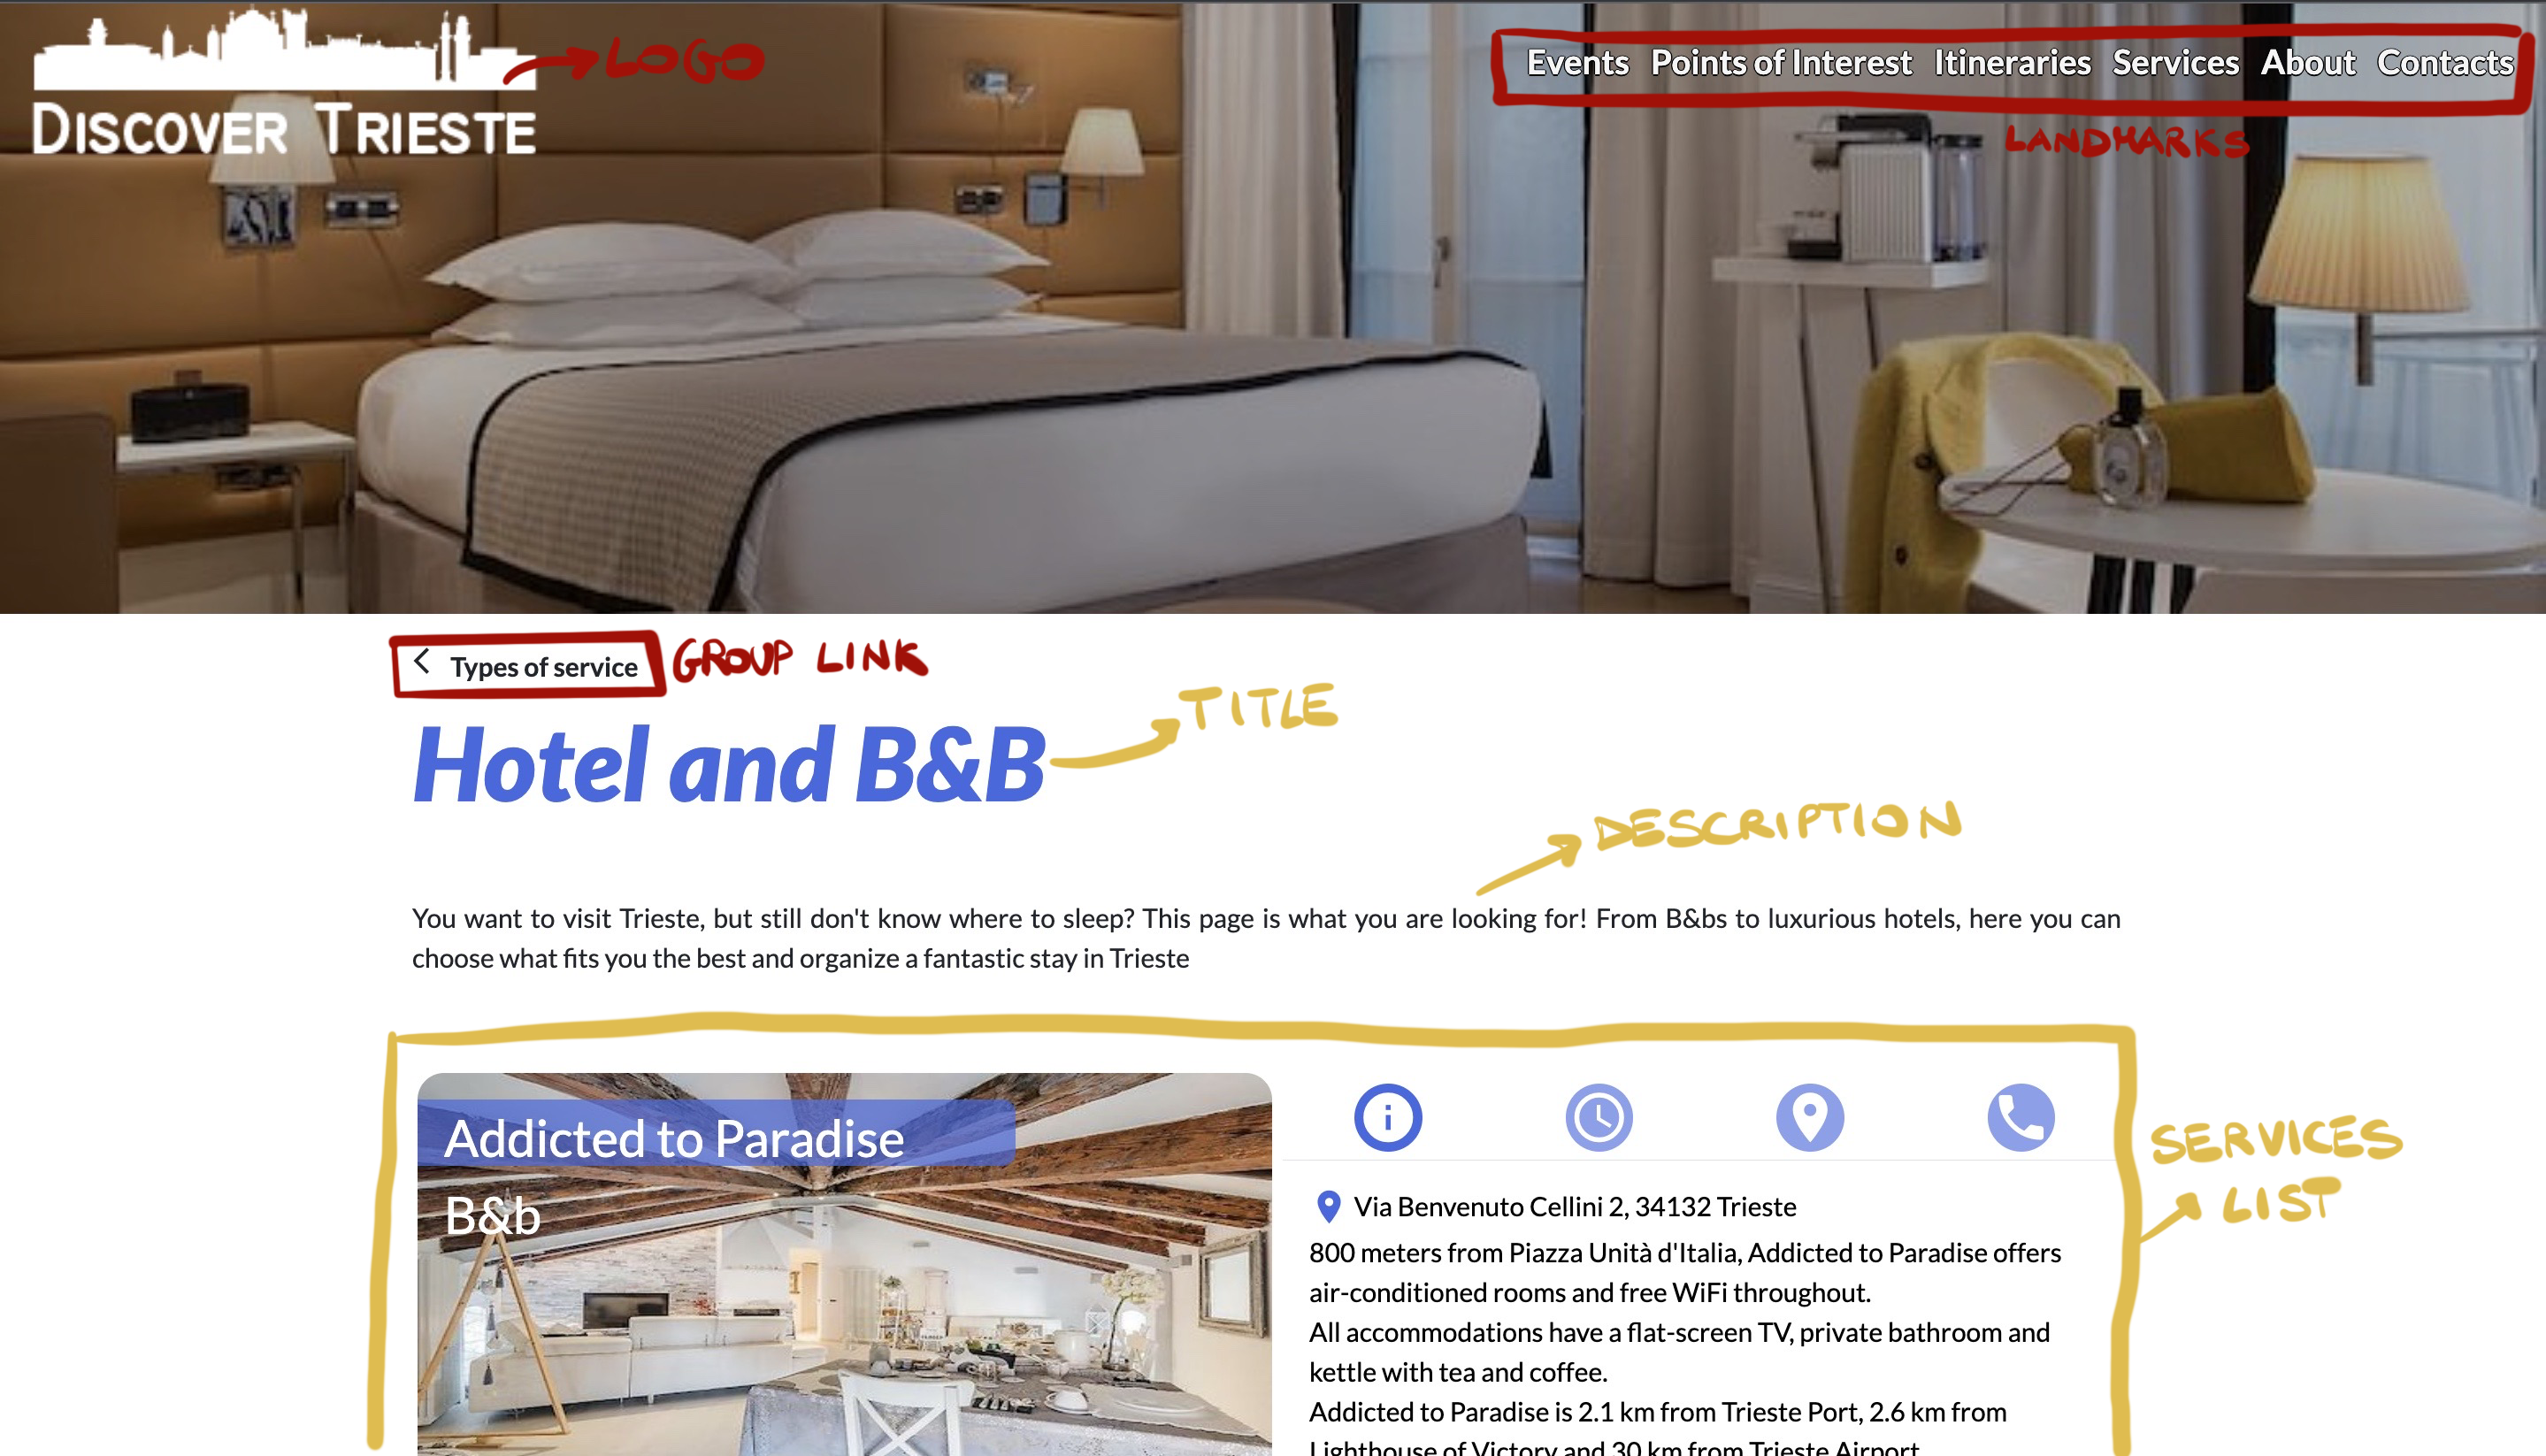
\includegraphics[width=\textwidth]{assets/Wireframes/service.png}
        \caption{Type of service (kind of topic) wireframe}
    \end{center}
\end{figure}

\begin{figure}[H]
    \begin{center}
        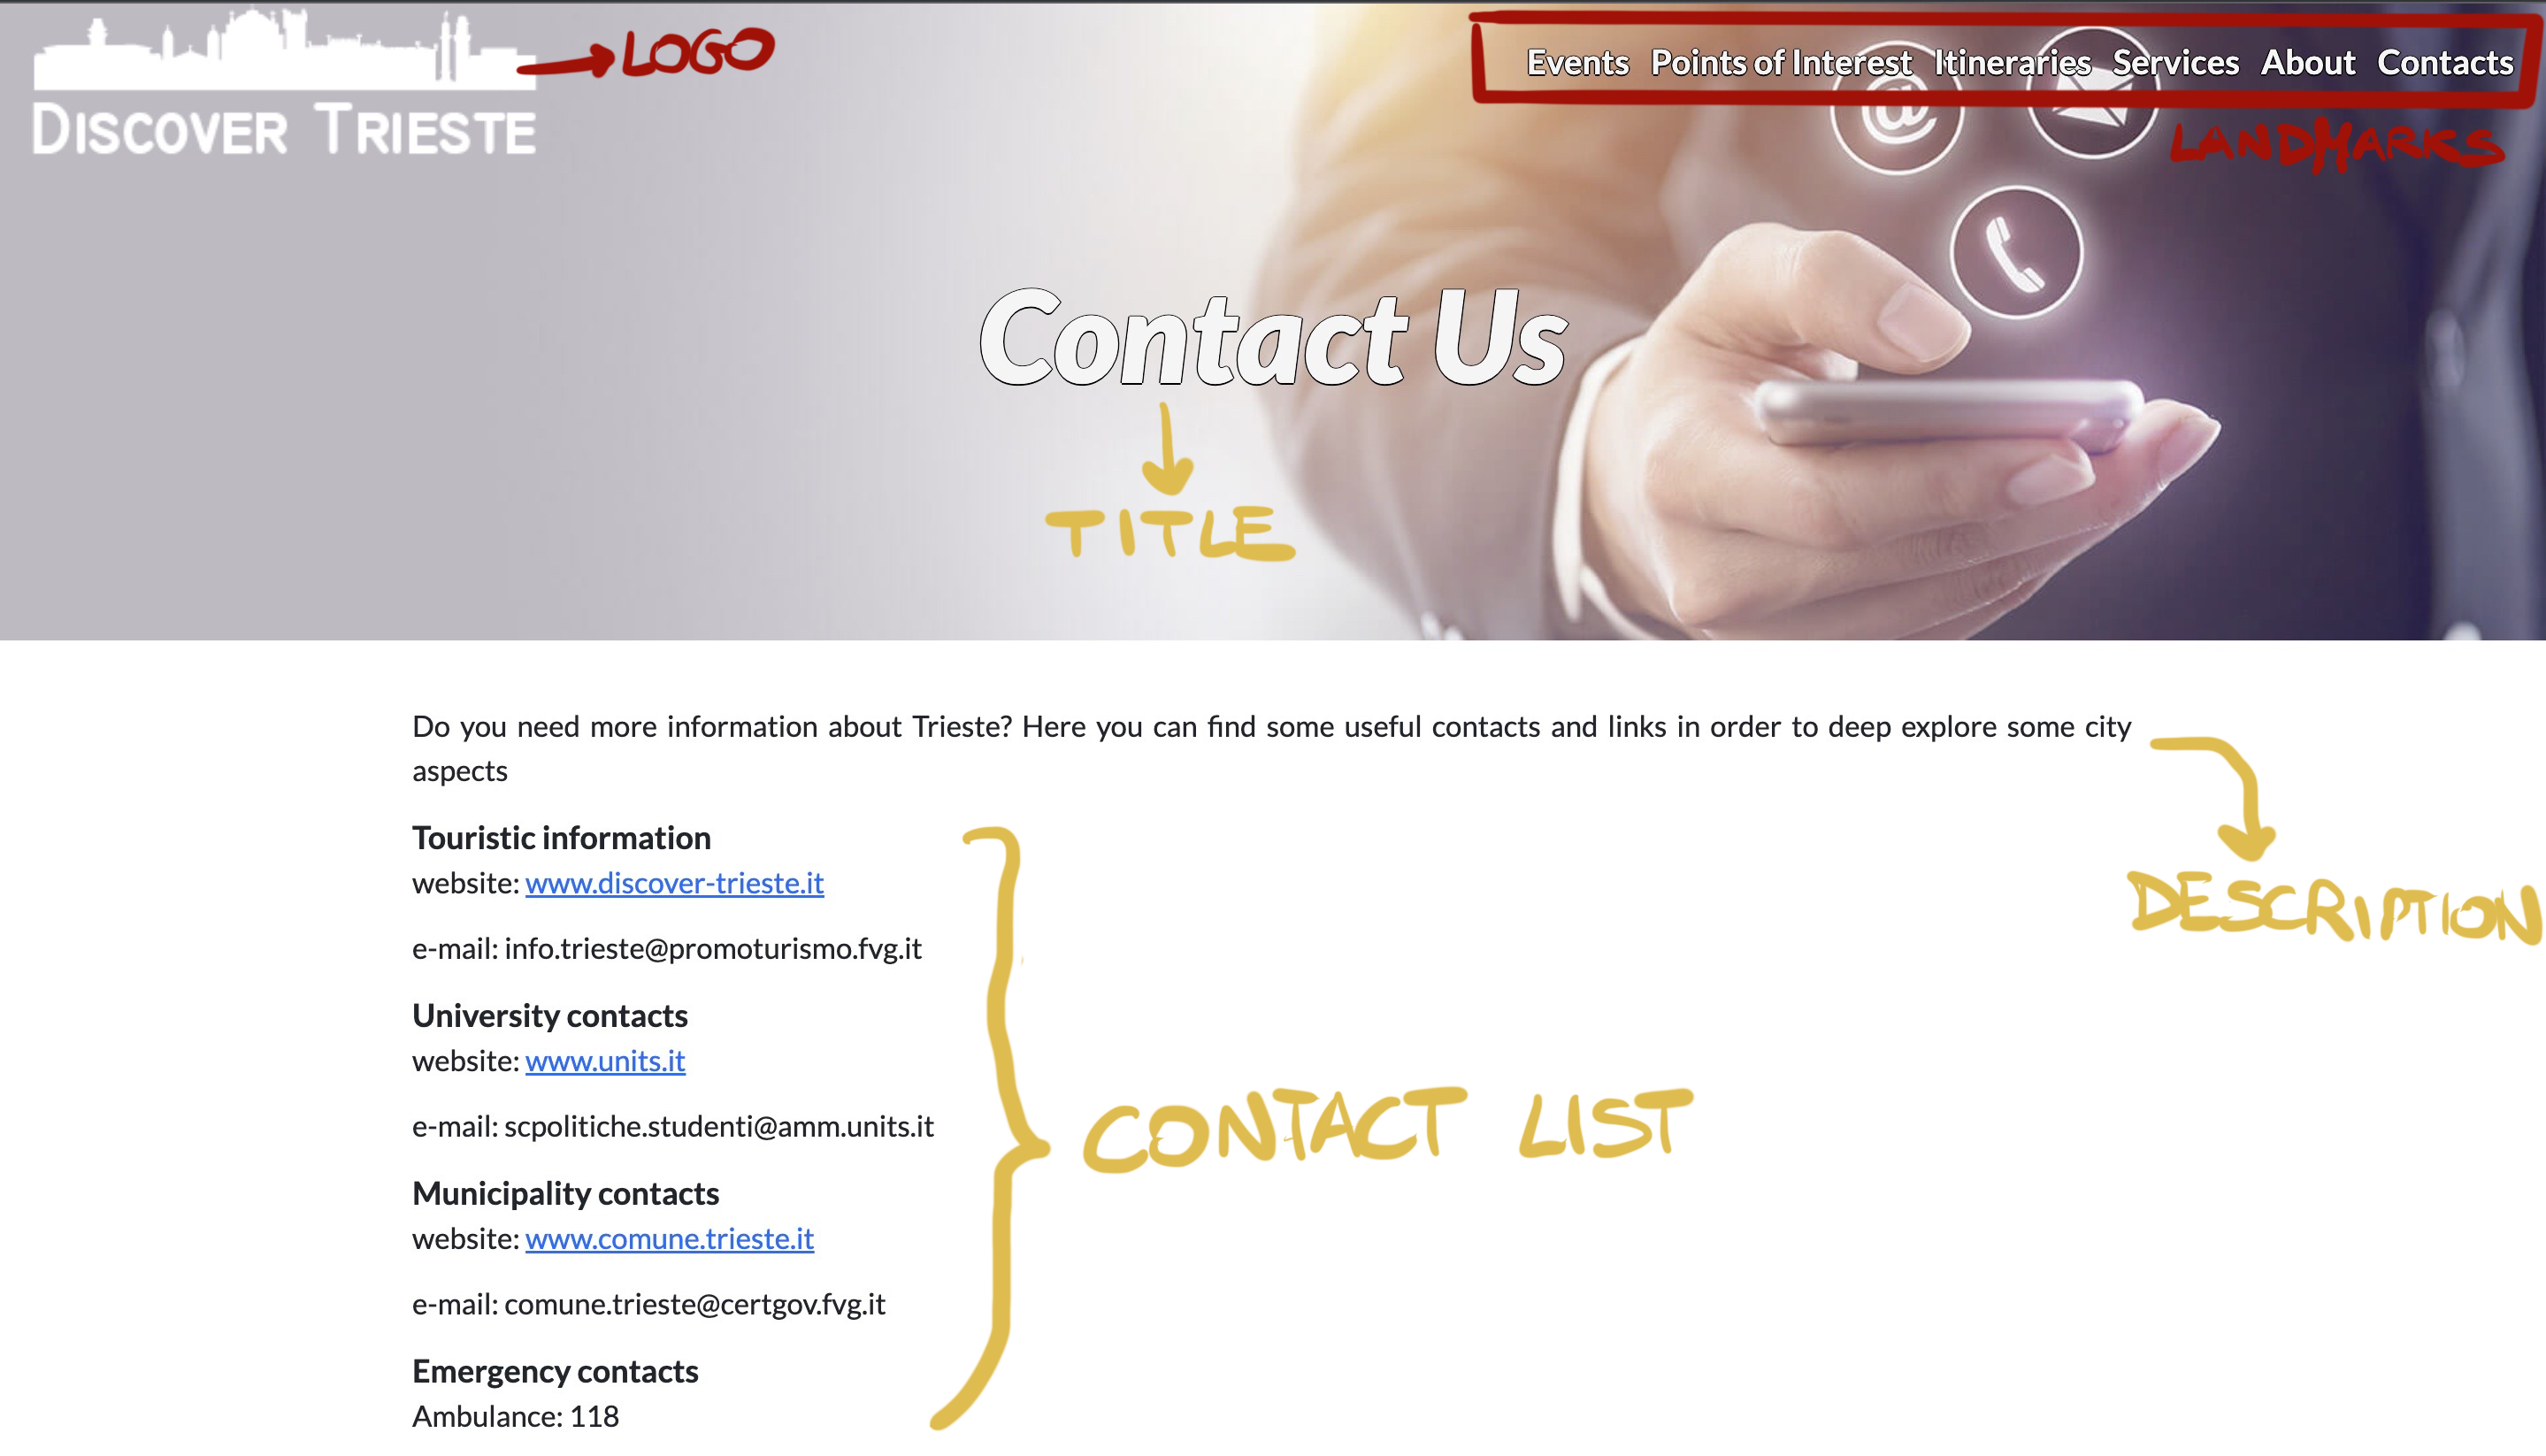
\includegraphics[width=\textwidth]{assets/Wireframes/contacts.png}
        \caption{Contacts wireframe}
    \end{center}
\end{figure}

In all the previous wireframes, the bottom of page was cut for space reason. Here there is a screenshot of the website footer which is present in all the pages.
\begin{figure}[H]
    \begin{center}
        
\includegraphics[width=\textwidth]{assets/Wireframes/footer.png}
        \caption{Footer wireframe}
    \end{center}
\end{figure}

\newpage
\section{Interaction scenarios}
In this section scenarios are showed in order to give a sense of use of the webpage we created.
\subsection{Scenario 1: a romantic escape}
\begin{figure}[H]
    \begin{center}
        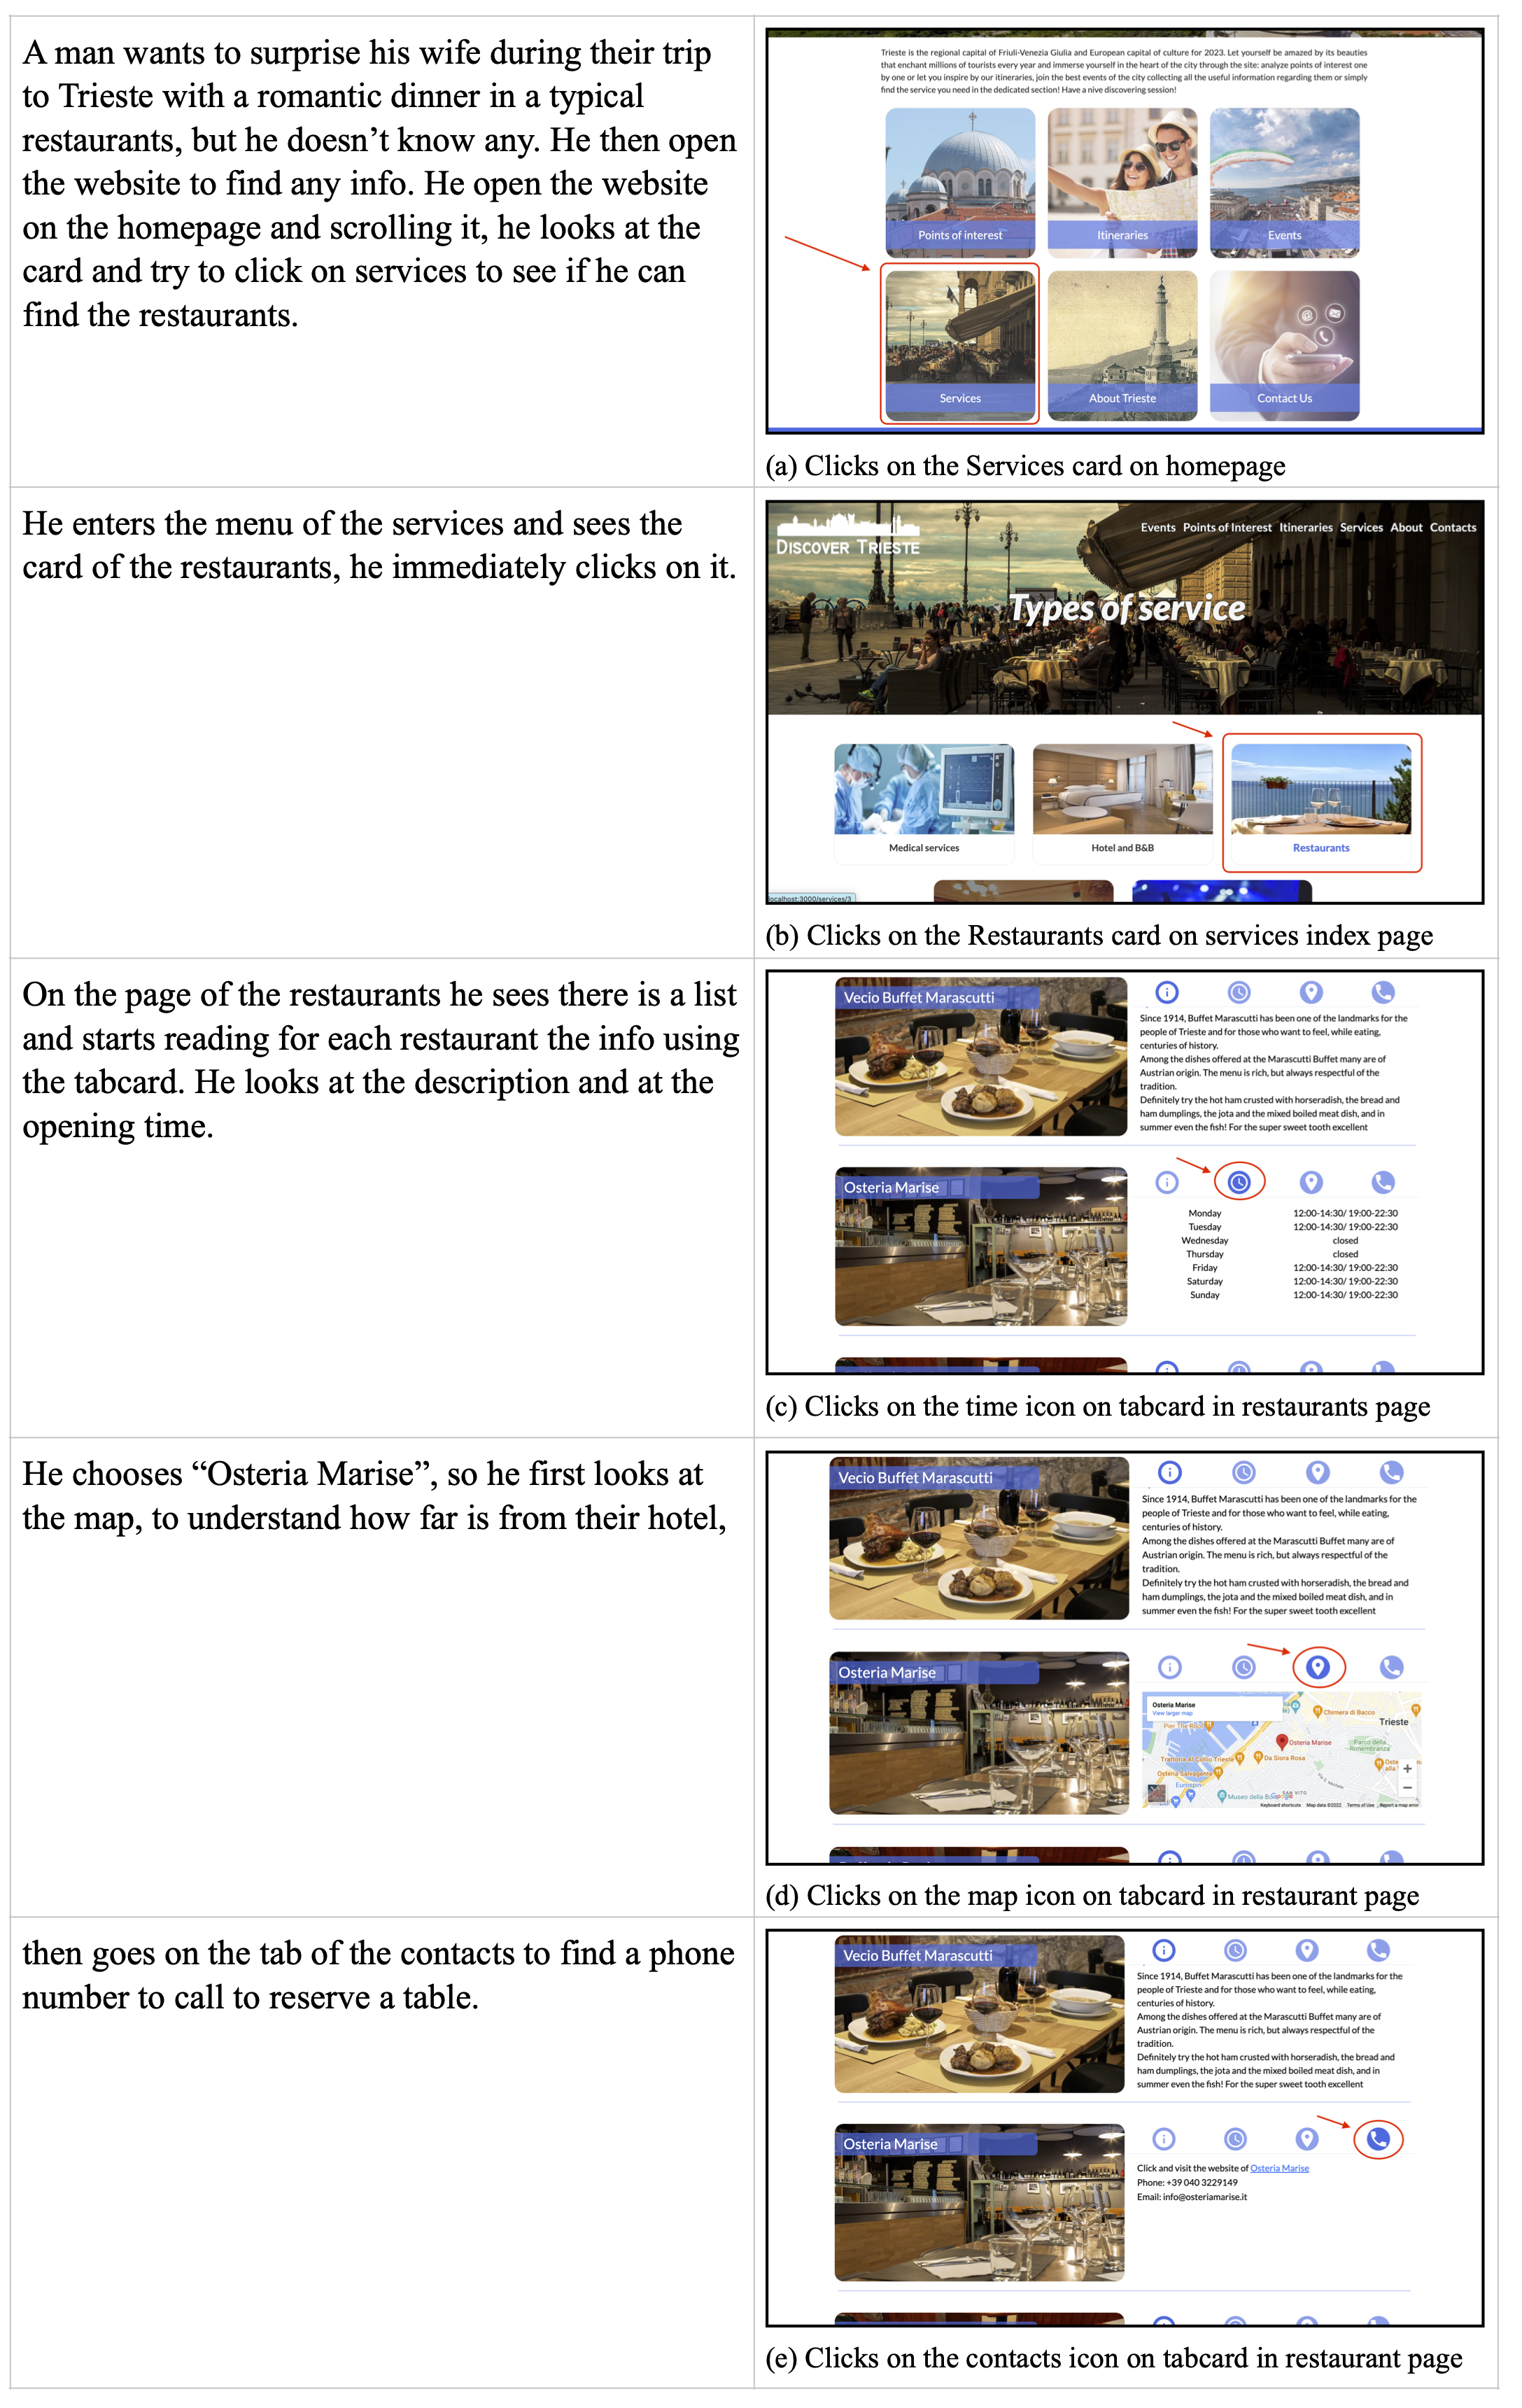
\includegraphics[width=0.9\textwidth]{assets/Scenarios/scenario1.png}
    \end{center}
\end{figure}
\subsection{Scenario 2: a Roman break}
\begin{figure}[H]
    \begin{center}
        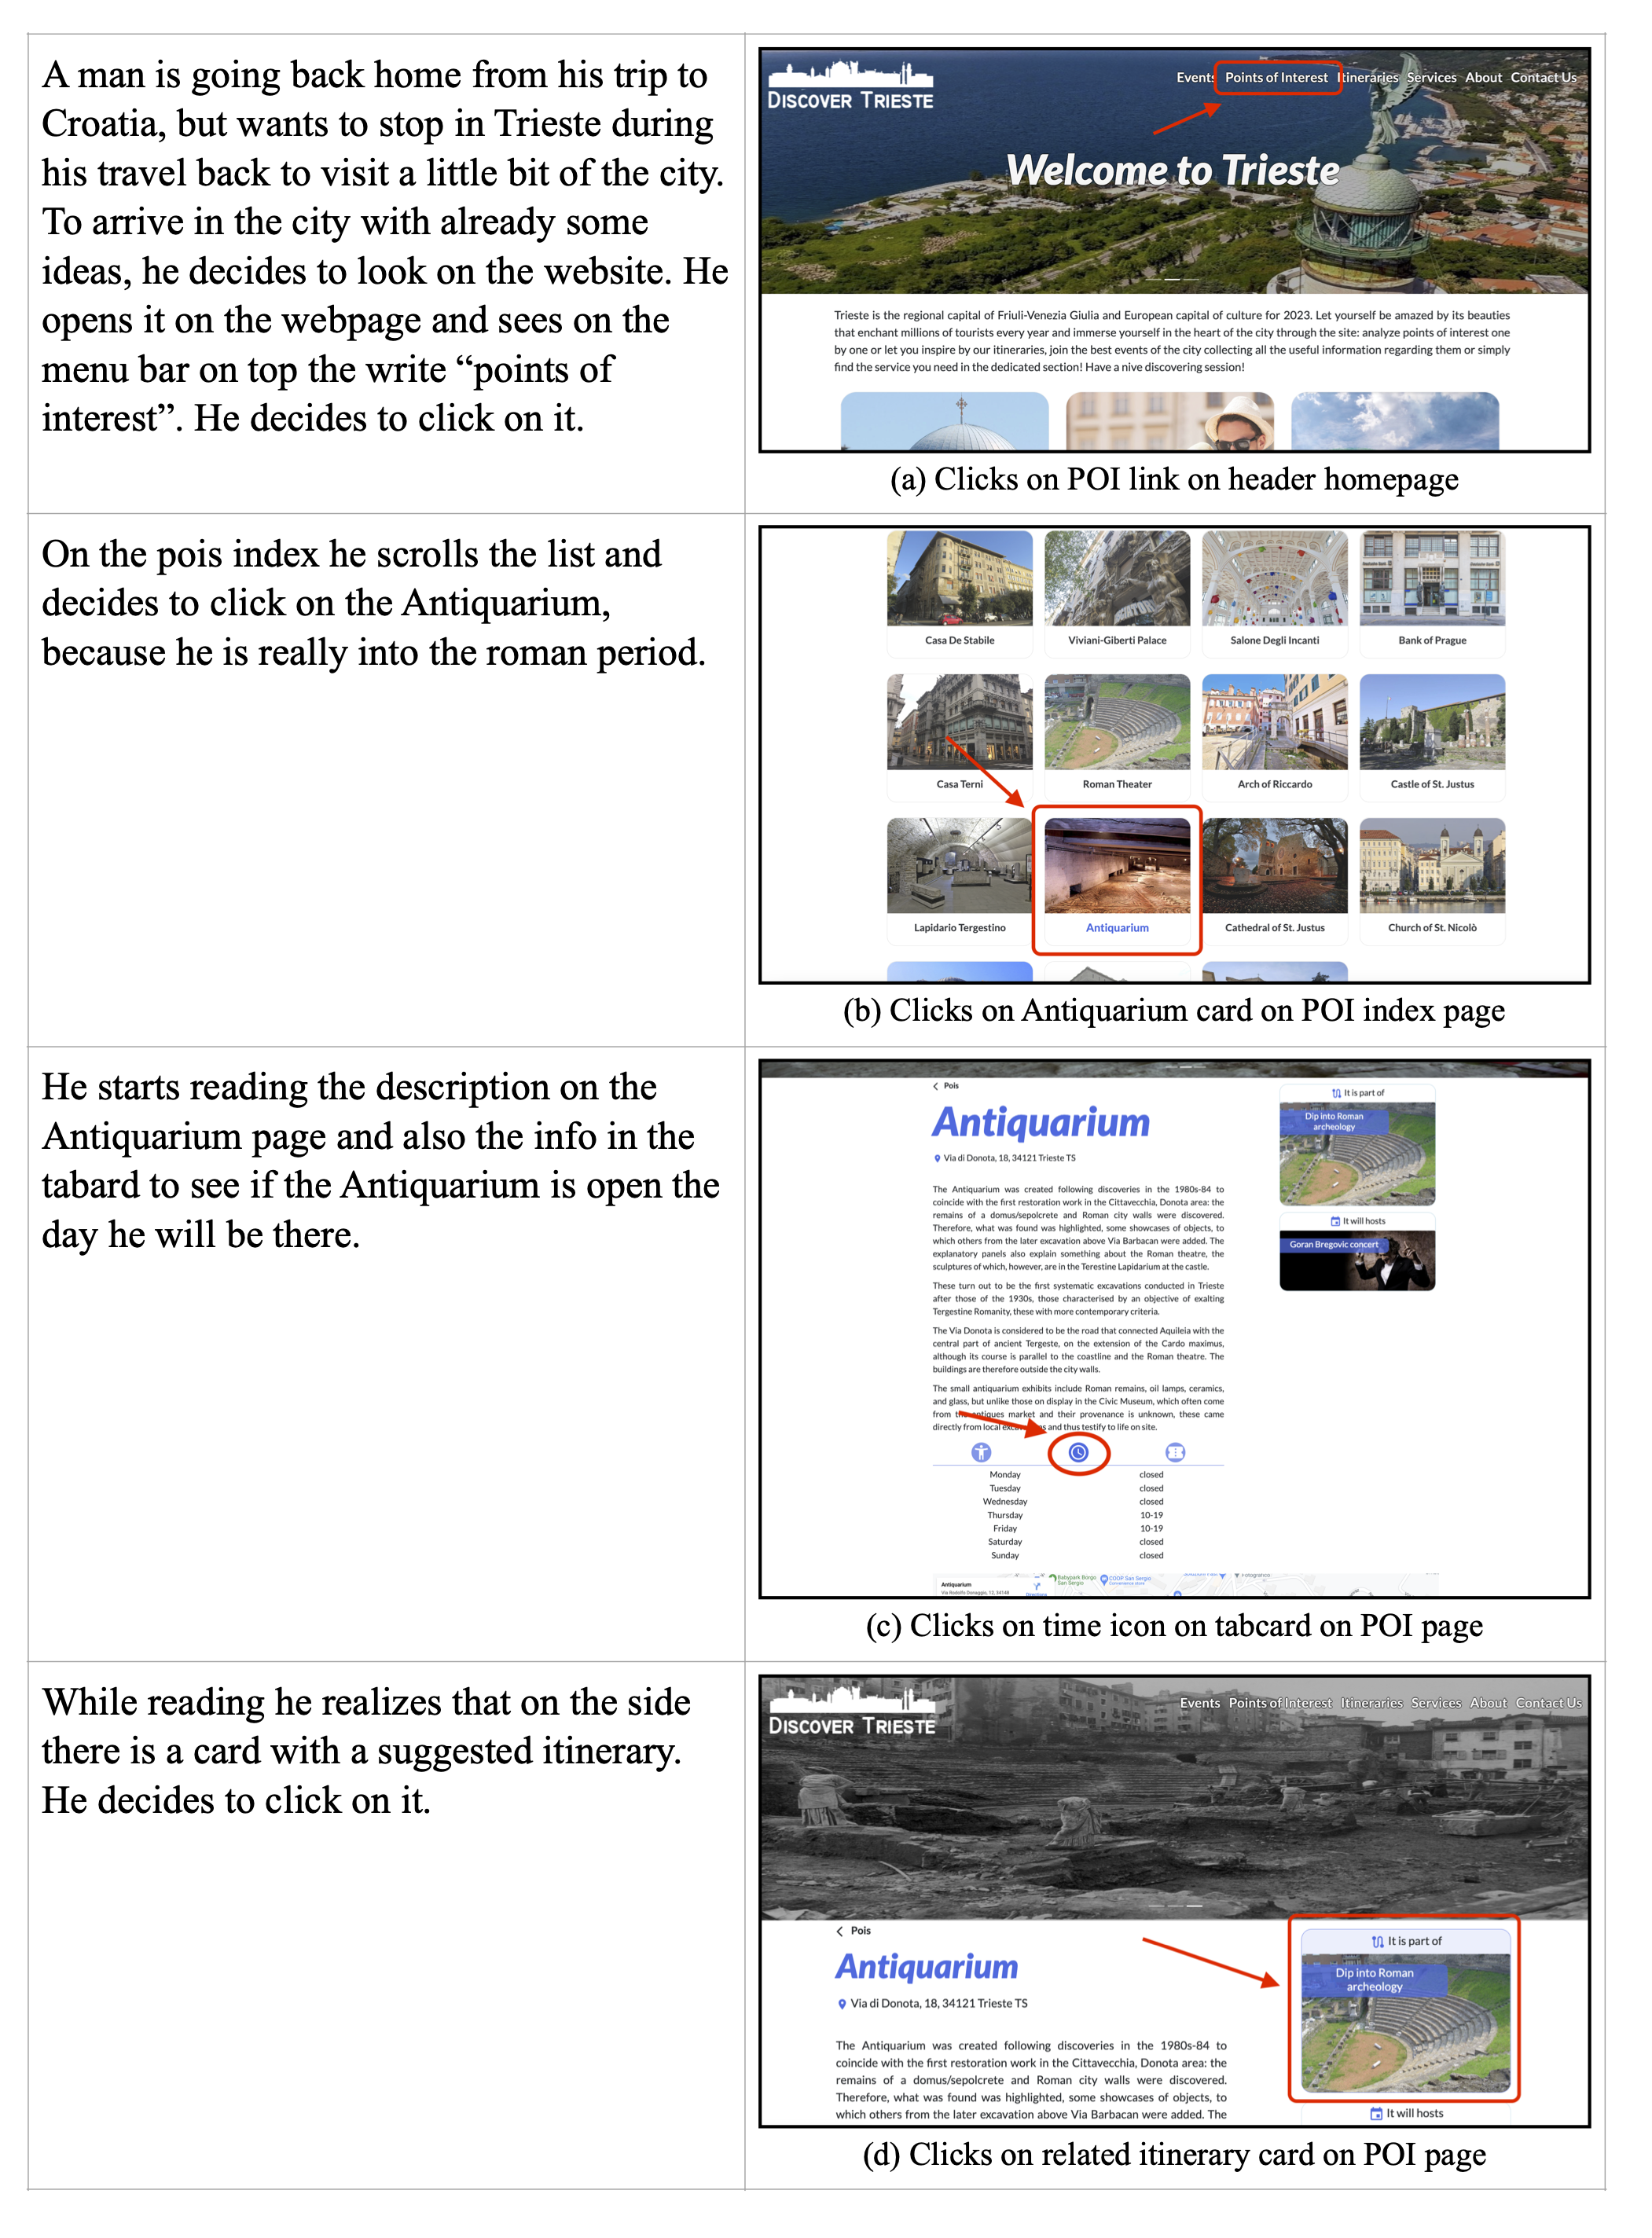
\includegraphics[width=0.9\textwidth]{assets/Scenarios/scenario2-1.png}
    \end{center}
\end{figure}

\begin{figure}[H]
    \begin{center}
        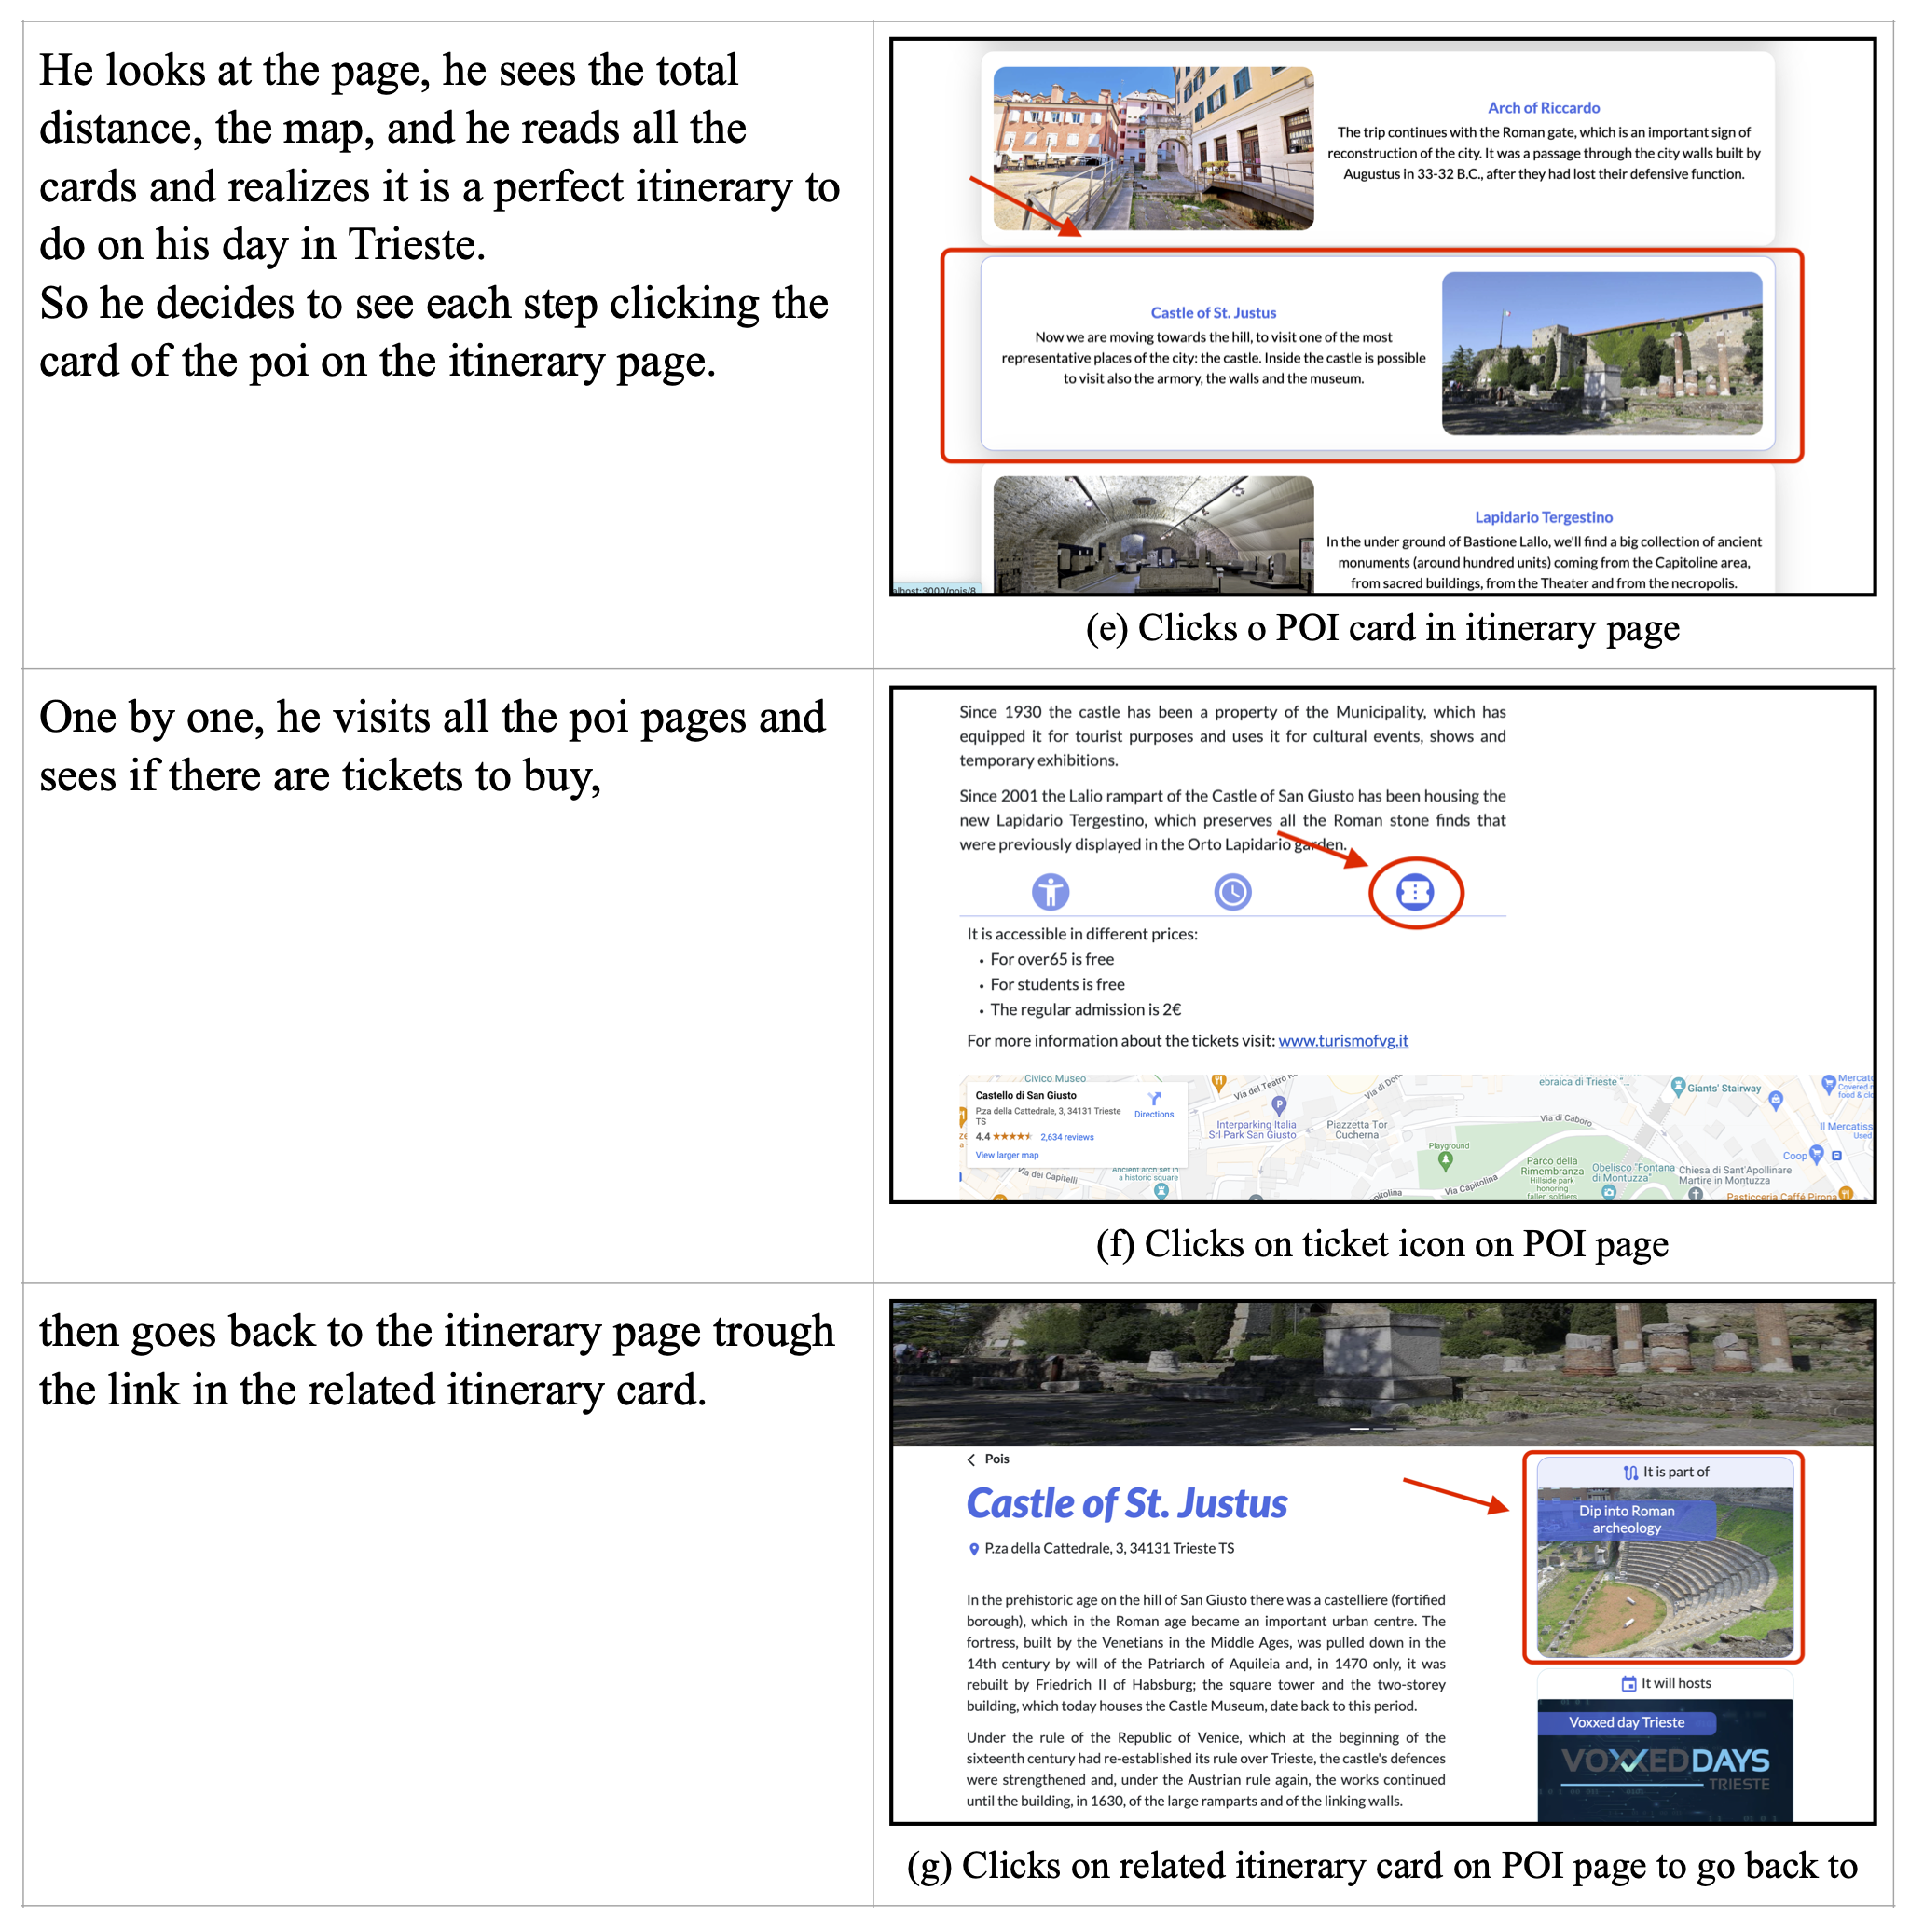
\includegraphics[width=0.9\textwidth]{assets/Scenarios/scenario2-2.png}
    \end{center}
\end{figure}

\subsection{Scenario 3: the school trip}
\begin{figure}[H]
    \begin{center}
        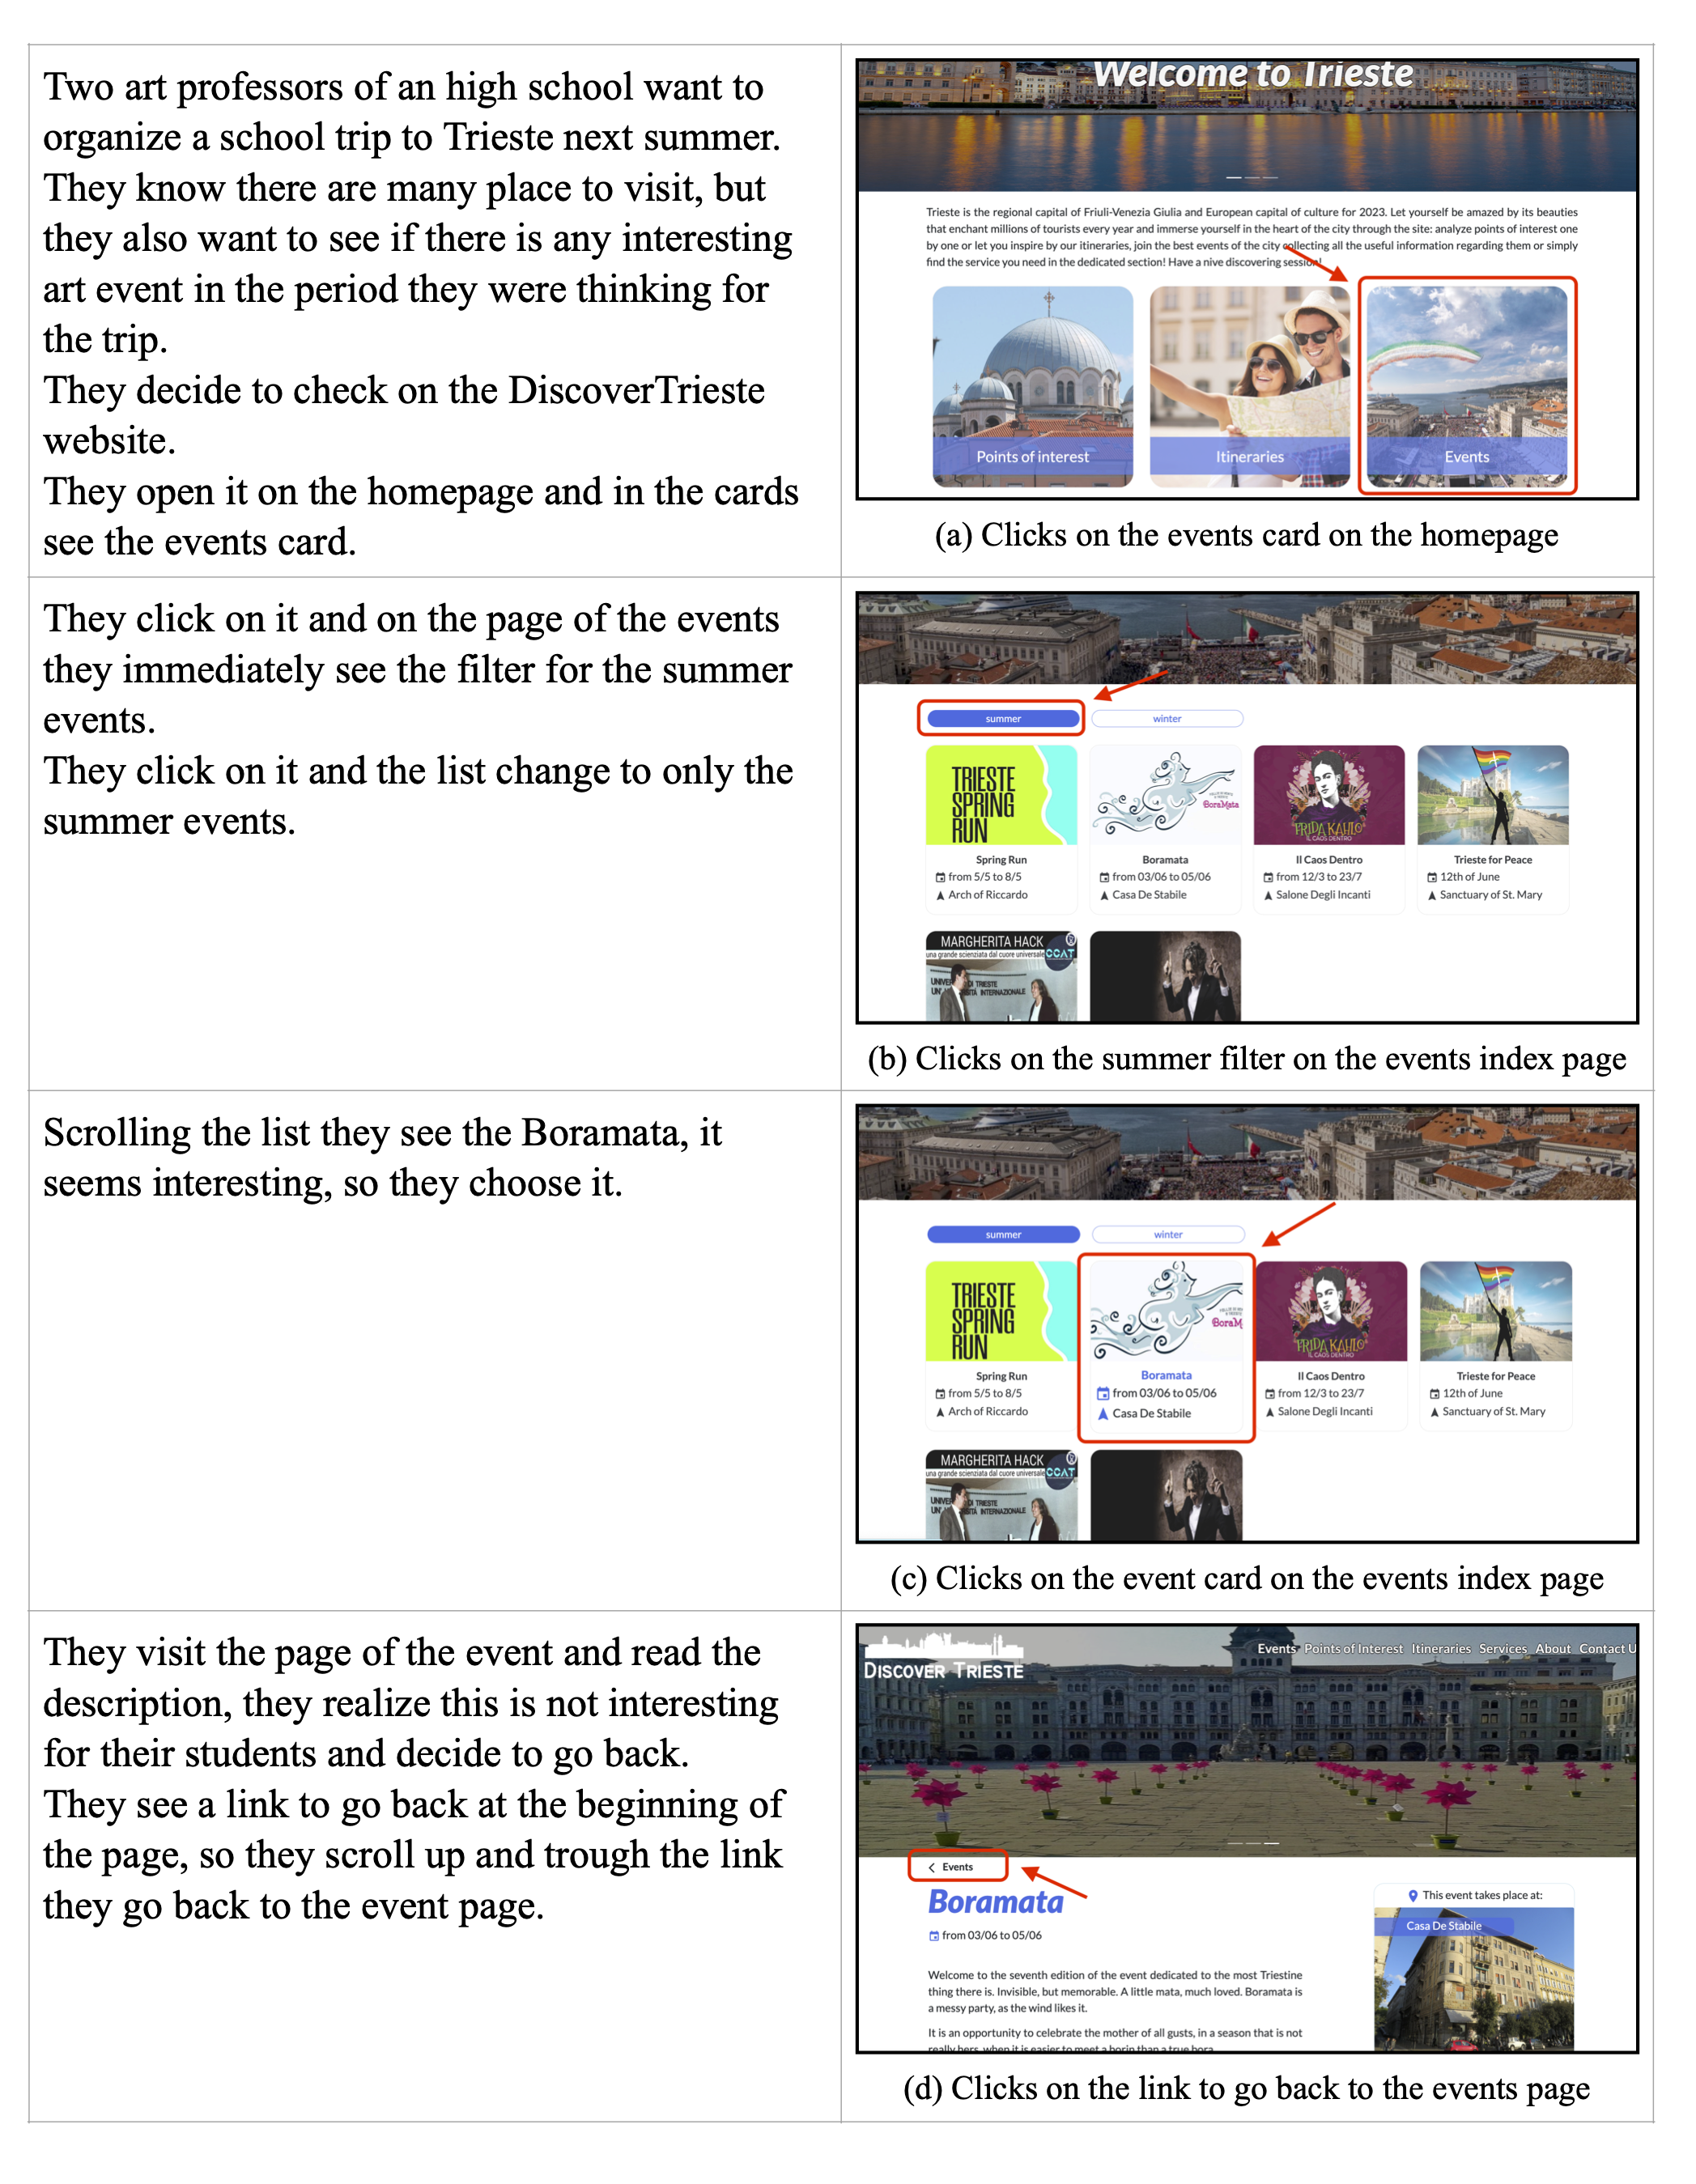
\includegraphics[width=0.9\textwidth]{assets/Scenarios/scenario3-1.png}
    \end{center}
\end{figure}

\begin{figure}[H]
    \begin{center}
        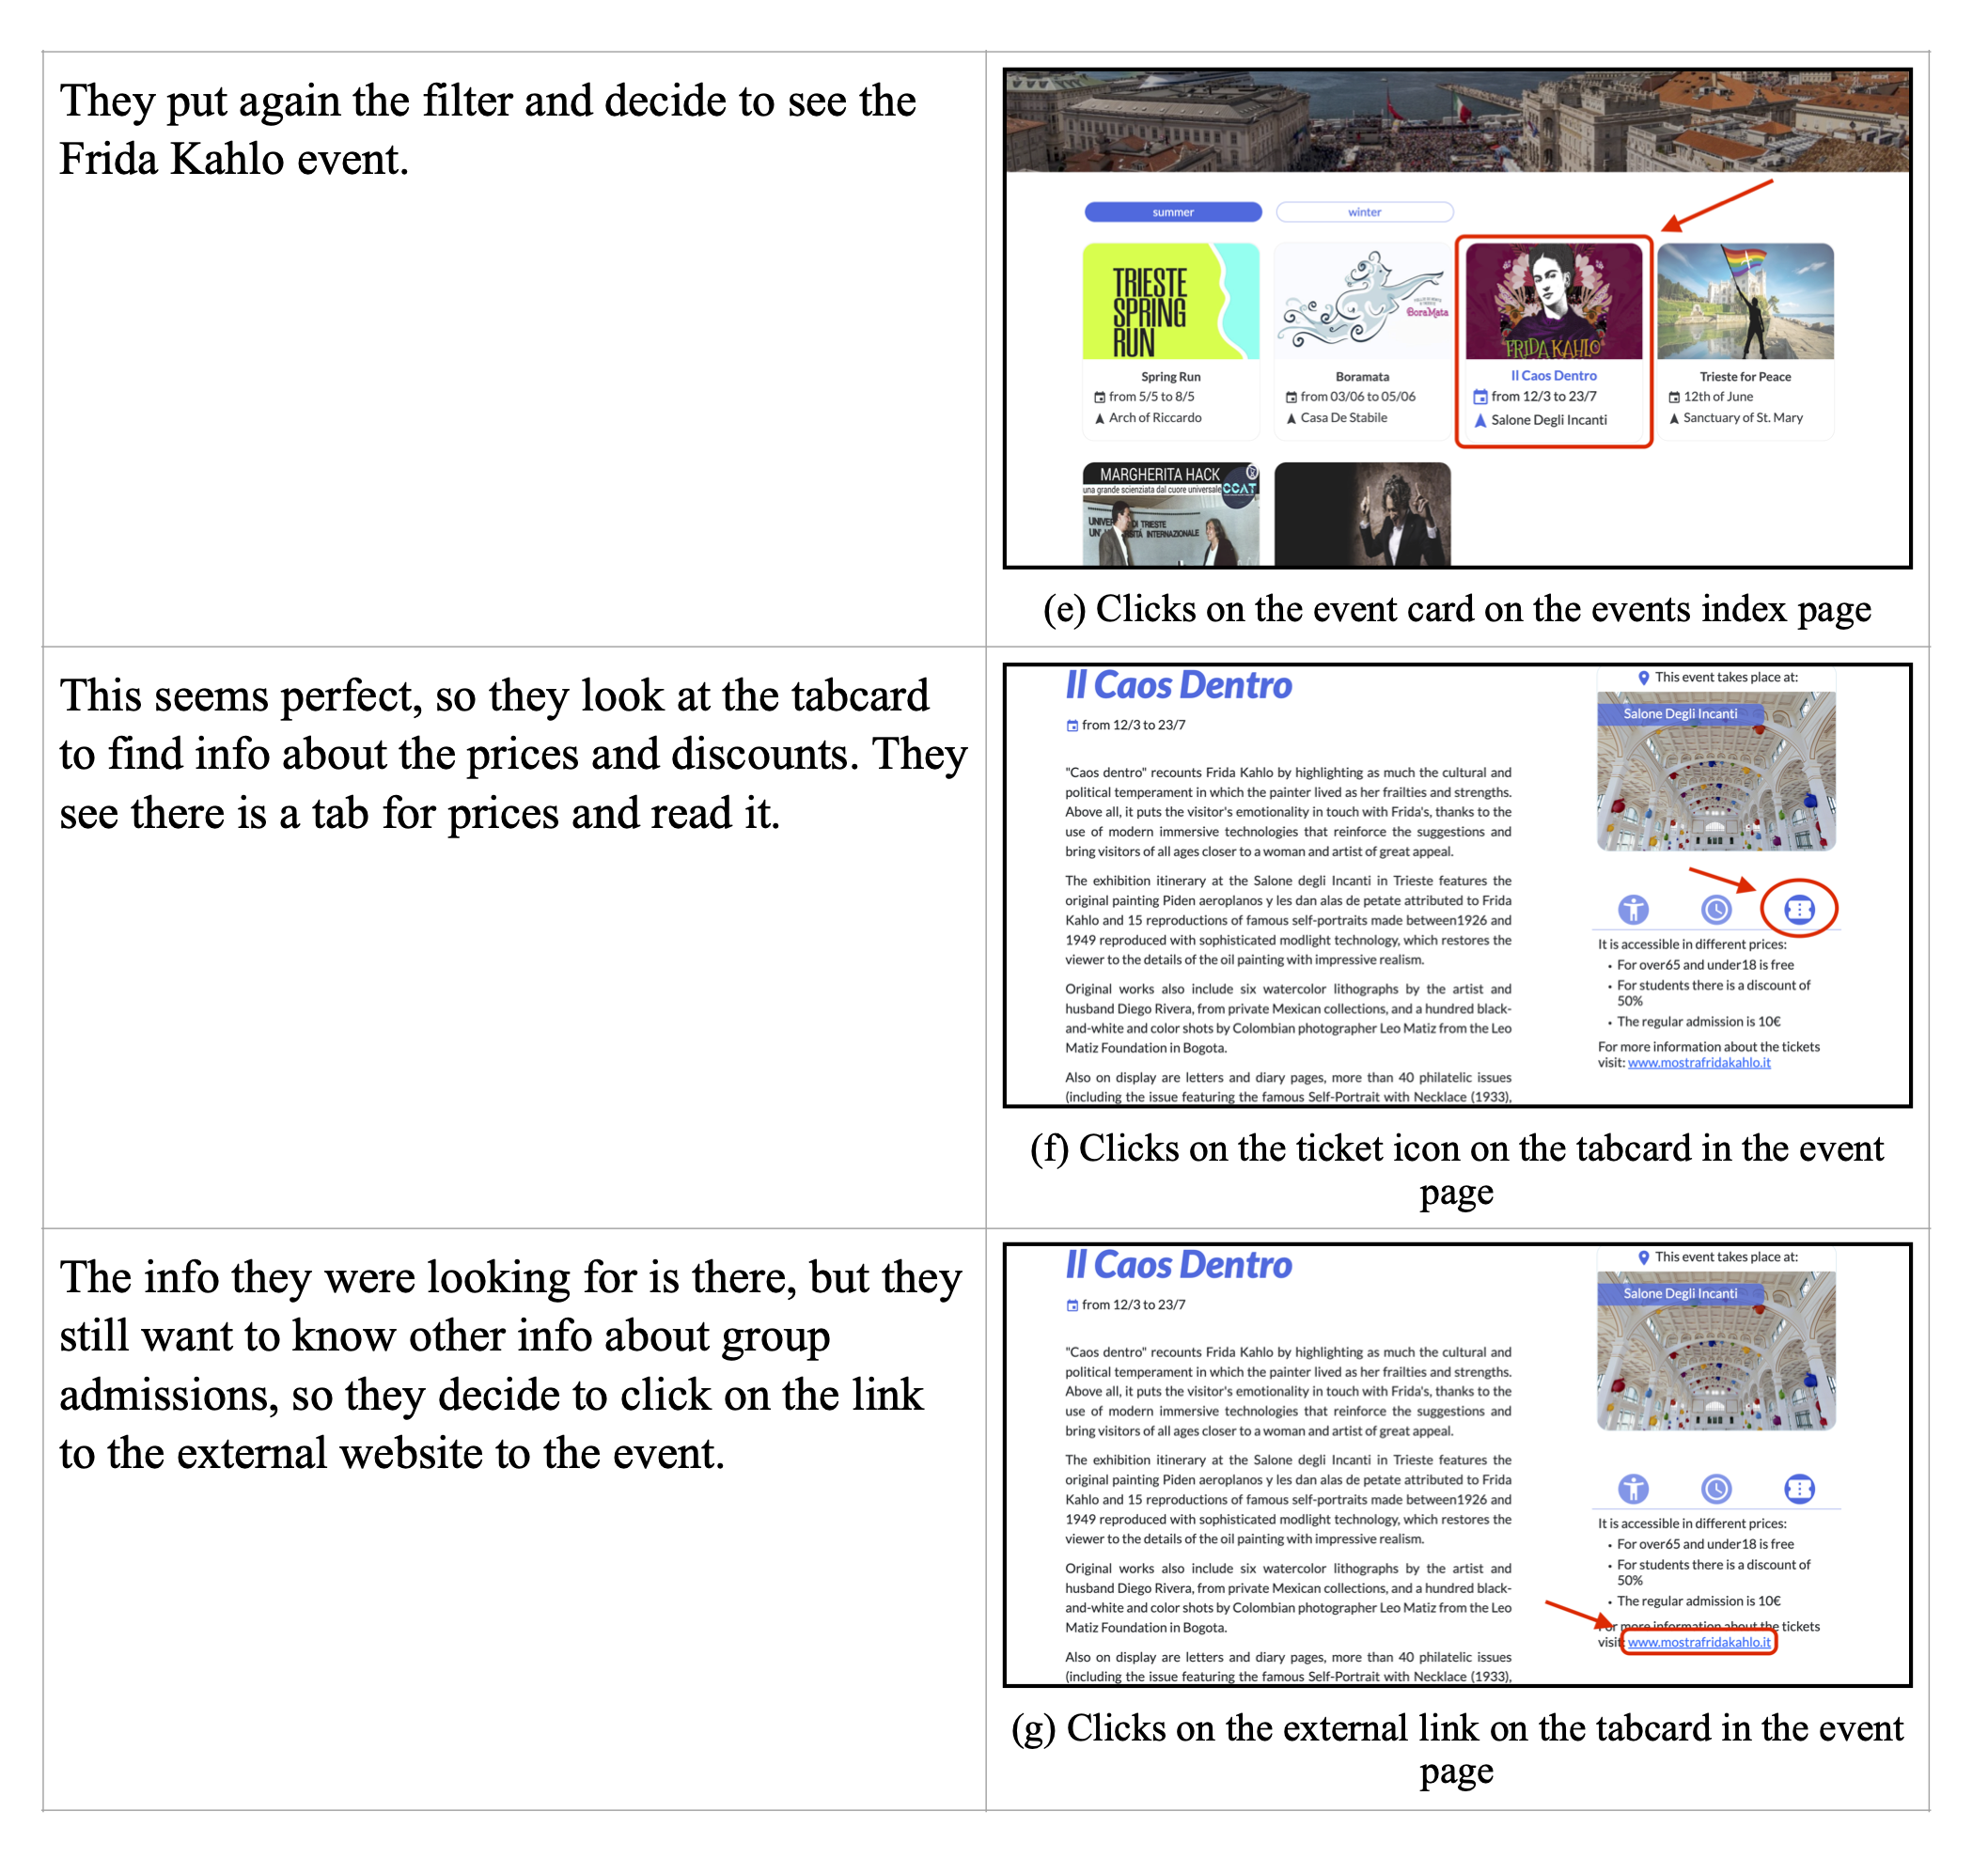
\includegraphics[width=0.9\textwidth]{assets/Scenarios/scenario3-2.png}
    \end{center}
\end{figure}

\section{Effort spent}
\begin{tabular}{ | c || c | c | c | c| c|}
    \hline
    Student           & Documentation   & Co-work     & Coding  \\ \hline
    Stefano Abatiello      & 2h          	   & 75h              & 49h            \\ \hline
    Alessandro Bianco    & 4h        	   & 75h              & 46h             \\ \hline
    Camilla Blasucci       & 2h          	   & 75h              & 45h          \\ \hline
    Stefano Taborelli       & 2h          	   & 75h              & 47h       \\ 
    \hline
\end{tabular}
\end{document}
